\documentclass[9pt,table,xcolor=dvipsnames]{beamer}% {{{
\input{Common-White.tex}
% }}}
  \title{Bridging the \textit{real} and \textit{imaginary} worlds}% {{{
% \subtitle
% {Research Plan} % (optional)

\author{Le Chen\\ \bigskip
Auburn University \\[2em]
}
% - Use the \inst{?} command only if the authors have different
%   affiliation.
\institute[Auburn University]
{%
% \pgfuseimage{Auburn}
% Jointwork with\\[1em]
% Raluca Balan, Xia Chen and Nicholas Eisenberg \\
 % \vspace{2cm}
 }
% - Use the \inst command only if there are several affiliations.
% - Keep it simple, no one is interested in your street address.

% \date[Talk at Karlsruhe] % (optional)
% {\today }
\date[Columbus]{
Stochastic Analysis Seminar\\ \bigskip
\: Auburn University\\[1em]
2022-04-19\\
}

% This is only inserted into the PDF information catalog. Can be left
% out.

% If you have a file called "university-logo-filename.xxx", where xxx
% is a graphic format that can be processed by latex or pdflatex,
% resp., then you can add a logo as follows:

\pgfdeclareimage[height=2cm]{Auburn}{figs/AU-Black.jpeg}

% Delete this, if you do not want the table of contents to pop up at
% the beginning of each subsection:
% \AtBeginSubsection[]
% {
%   \begin{frame}<beamer>{Outline}
%     \tableofcontents[currentsection,currentsubsection]
%   \end{frame}
% }

% If you wish to uncover everything in a step-wise fashion, uncomment
% the following command:

% \beamerdefaultoverlayspecification{<+->}

\begin{document}
% }}}
\begin{frame}[noframenumbering] % Title page.
  \titlepage
\end{frame}
\begin{frame}{Plan} % TOC
 \tableofcontents
\end{frame}
\section{A bird view of SPDEs and the two worlds}
\begin{frame}[fragile,t] % Surface growth -- Cell
  \frametitle{Surface growth}

  \begin{center}
    Rule of replication of \textcolor{cyan!80!black}{\bf cells}
    \footnote{
      \textcolor{refcolor}{S. Santalla and S. Ferreira}.
    % Eden model with nonlocal growth rules and kinetic roughening in biological systems.
    {\it  Phys. Rev. E.} 98, 2018} \\[1em]
    Replication probability $\propto$ Aperture angle \textcolor{red}{\bf $\theta_i$}
    % depends on the \textcolor{gray}{empty space} \\
    % bridging its position at the colony and  \\
    % the outer medium of the culture
  \end{center}

\bigskip
  \begin{center}
    \begin{minipage}{0.4\textwidth}
      \begin{center}
	\textcolor{gray}{\tiny Microscopic world}

	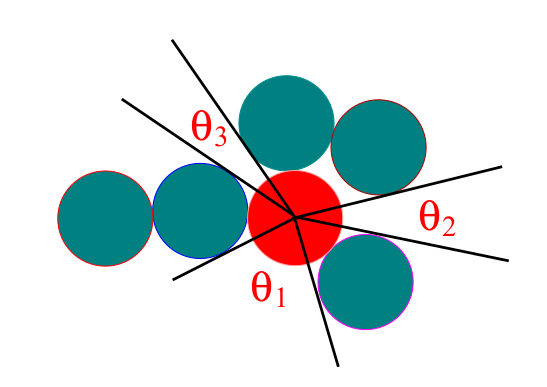
\includegraphics[scale=0.2]{figs/Eden-Mechanism.png}
	\bigskip

	\only<2->{Some rules}
      \end{center}
    \end{minipage}
    \hspace{2em}
    $\Rightarrow$
    \begin{minipage}{0.4\textwidth}
      \begin{center}
	\textcolor{gray}{\tiny Macroscopic world}
	\medskip

	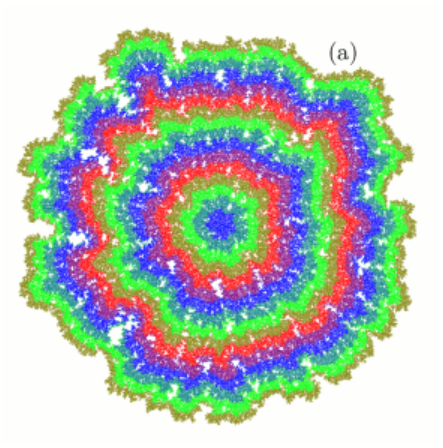
\includegraphics[scale=0.2]{figs/Eden-Simulation-a.png}

	\only<3->{\alert{Universal object -- KPZ!}}
      \end{center}
    \end{minipage}
  \end{center}

\small \vfill \pause \pause \pause

  \begin{align}
    \tag{KPZ}
    \dfrac{\partial}{\partial t} h(t,x) = \frac{1}{2} \Delta h(t,x) + \frac{\lambda}{2} \left(\nabla h\right)^2 +\textcolor{contrast_color_1}{\dot{W}(t,x)}
  \end{align}
\end{frame}
\begin{frame}[fragile] % Surface growth -- DMS
  \frametitle{Study of growing interfaces in a thin film \\
    \small --- Convection of nematic liquid crystal \footnote{
      \textcolor{refcolor}{K. Takeuchi, M. Sano, T. Sasamoto {\it et al}}. {\it Sci. Rep. (Nature)}, 1, 34 (2011).
      % Growing interfaces uncover universal fluctuations behind scale invariance.
  }}

  \begin{center}
    \only<1>{Show movies~!}
    \only<2>{
      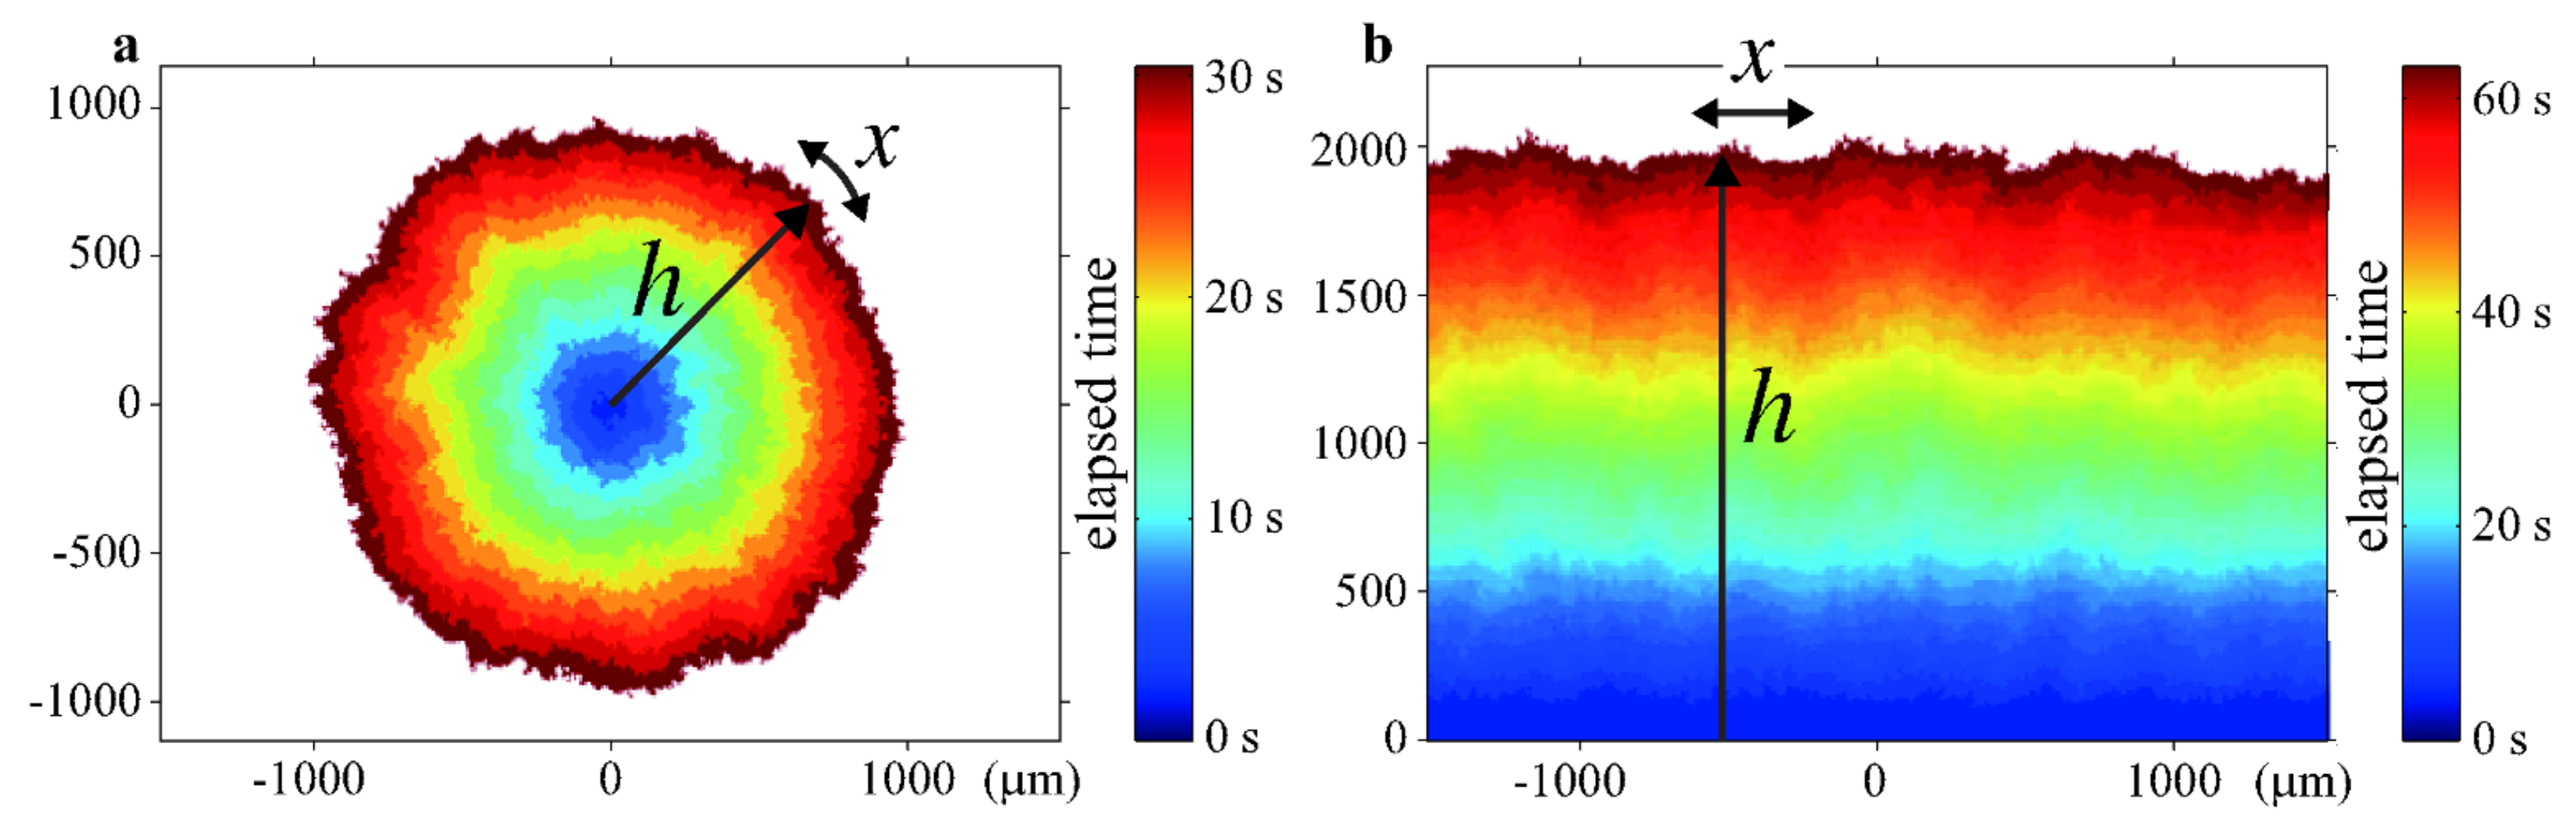
\includegraphics[scale=0.08]{./figs/Growing-DSM2.png}

      \vfill
      Prediction from KPZ equation:
      \begin{align*}
        h\asymp v_\infty t + \left(\Gamma t\right)^{1/3} \xi
      \end{align*}
    }
    \only<3>{
      \begin{align*}
        h\asymp v_\infty t + \left(\Gamma t\right)^{1/3} \xi
      \end{align*}
      \bigskip

      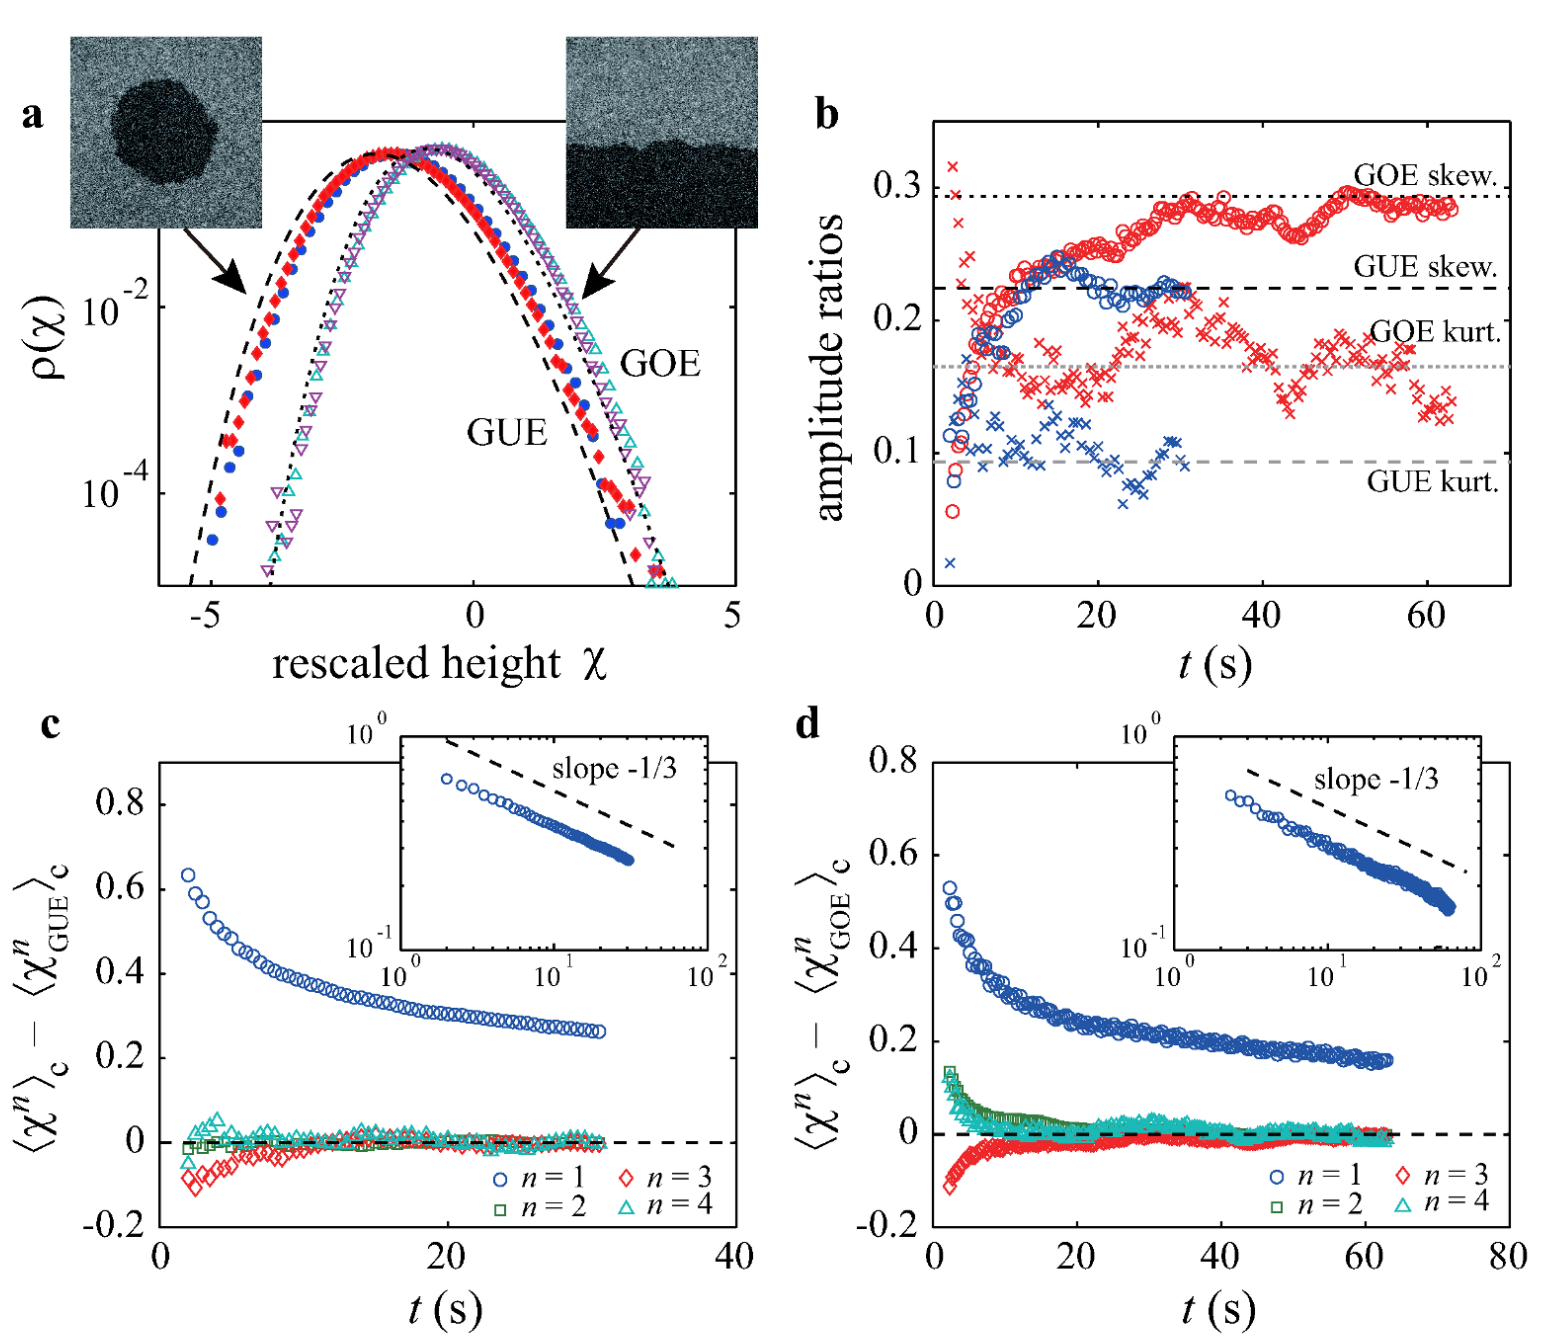
\includegraphics[scale=0.12]{./figs/Universal_Fluctuations_DSM.png}
    }
  \end{center}

\end{frame}
\begin{frame}[fragile] % KPZ three authors' photos
  \frametitle{KPZ Equation '86 \footnote{"Dynamic Scaling of Growing Interfaces". Physical Review
  Letters. 56 (9): 889--892, 1986.}}

  \begin{center}
    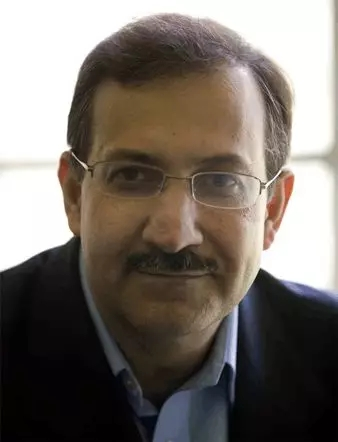
\includegraphics[scale=0.22]{figs/Kardar.jpg}
    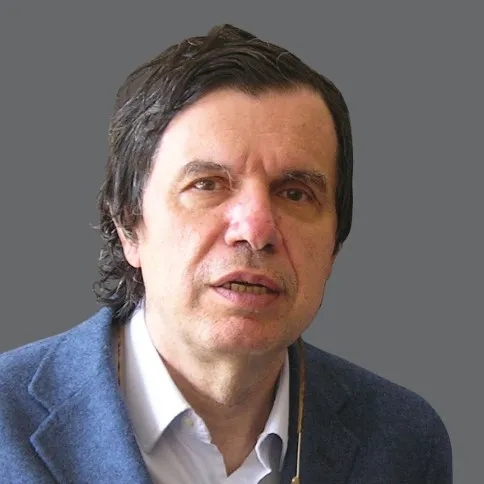
\includegraphics[scale=0.20]{figs/Parisi.jpg}
    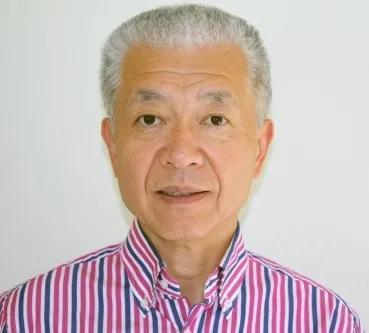
\includegraphics[scale=0.28]{figs/Zhang.jpg}
  \end{center}

  \small
  \quad Mehran Kardar (1957 --) \:\:  Giorgio Parisi (1948 --) \qquad\qquad Yicheng Zhang
\end{frame}
\begin{frame}[fragile] % Parisi -- Nobel
 \begin{center}
  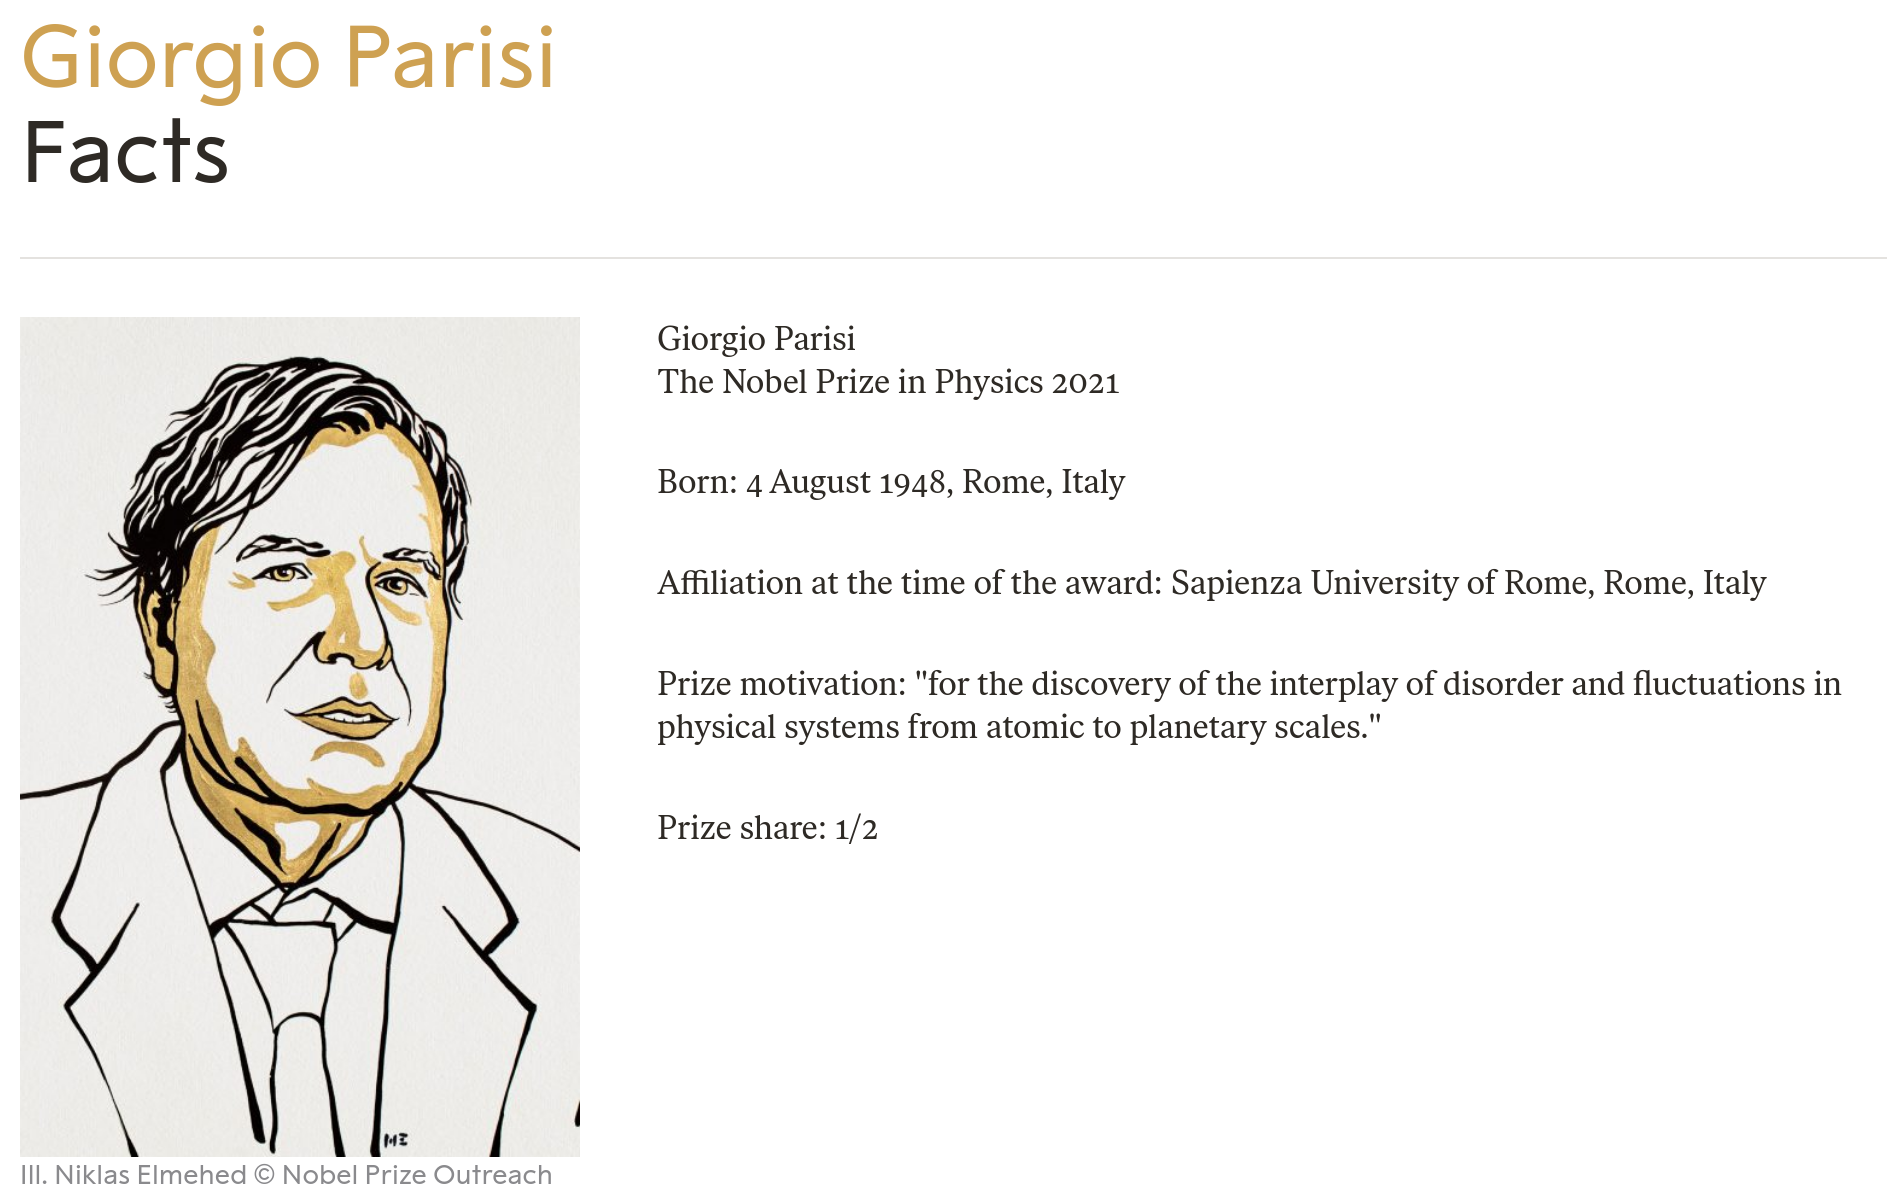
\includegraphics[scale=0.15]{figs/Parisi.png}
  \bigskip

  \small
  \url{https://www.nobelprize.org/prizes/physics/2021/parisi/facts/}
   % \begin{tikzpicture}[scale=1, transform shape]
   %   \node (fig) at (0,0) {};
   %   \pause
   %   \draw[red] (-3,-0.33) rectangle ++(6,+3) node [right] {Group $X$};
   %   \pause
   %   \draw[red] (-3,-0.36) rectangle ++(6,-3) node [right] {Group $Y$};
   % \end{tikzpicture}
 \end{center}
\end{frame}
\begin{frame}<4>[fragile] % Hairer
  \begin{minipage}{0.3\textwidth}
  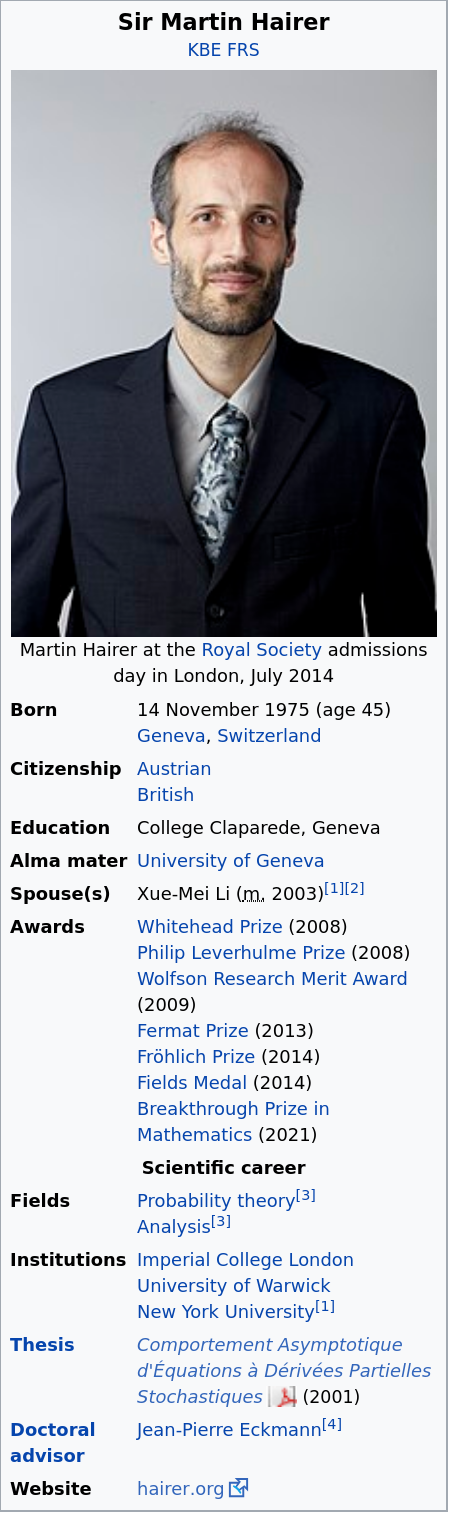
\includegraphics[scale=0.15]{figs/Hairer.png}
  \end{minipage}
  \begin{minipage}{0.65\textwidth}
    \pause
    \begin{itemize}
      \small
      \item \textcolor{refcolor}{M. Hairer}. Solving the KPZ equation. {\it Annals of Mathematics}, vol. 178, 2013.
        \bigskip
      \item \textcolor{refcolor}{M. Hairer}. A theory of regularity structures. {\it Inventiones mathematicae}, vol. 198, 2014.
        \bigskip
        \mySeparateLine
        \bigskip
      \item[]
        \begin{center}
          \Large
          Fields Medal in 2014
        \end{center}
    \end{itemize}
  \end{minipage}
\end{frame}
% {{{ 5. Mindmap SHE vs SWE
\tikzset{
  invisible/.style={opacity=0},
  visible on/.style={alt={#1{}{invisible} }},
  alt/.code args={<#1>#2#3}{%
    \alt<#1>{\pgfkeysalso{#2}}{\pgfkeysalso{#3}} % \pgfkeysalso doesn't change the path
  },
}
\begin{frame}

\begin{tikzpicture}[small mindmap, outer sep=0pt, text=white]

\begin{scope}[concept color=contrast_color_2!80!white]
\node (left) at (-2.2,0) [concept] {Stochastic Heat Equation}
  [counterclockwise from=110]
  child[visible on=<2->] { node[concept] {Surface growth (KPZ-equation)}  }
  child[visible on=<3->] { node[concept] {Stratified structure of universe} }
  child[visible on=<4->] { node[concept] {Parabolic Anderson model} }
;
\end{scope}

\begin{scope}[concept color=contrast_color_1!80!white]
\node (right) at (2.2,0) [concept] {Stochastic Wave Equation}
  [clockwise from=70]
  child[visible on=<5->] { node[concept] {Guitar string in sandstorm} }
  child[visible on=<6->] { node[concept] {Lake surface perturbed by rain} }
  child[visible on=<7->] { node[concept] {Electromagnetic field in a storm} }
;
\end{scope}

% \only<8>{\path (left) to[circle connection bar switch color=from (contrast_color_2!80!black) to (contrast_color_1!80!black)] (right) ;}
\end{tikzpicture}
\end{frame}
% }}}
\begin{frame}[fragile,t] % Smoothing vs Roughening
  \[
    \displaystyle\frac{\partial^b}{\partial t^b}u(t,x) = \left(\frac{1}{2}\Delta  + \dot{W}(x)\right) u(t,x)
  \]
  \begin{align*}
    \textcolor{contrast_color_2!80!black}{b=1: \text{SHE}} \qquad \textcolor{contrast_color_1!80!black}{b=2: \text{SWE}}
  \end{align*}
  \vspace{-1.8em}
   \begin{center}
    \begin{tikzpicture}
    \path (0,0) rectangle (0.35\paperwidth,0.4\paperheight);
    \node[scope fading=north,inner sep=0pt,outer sep=0pt,anchor=center] at(0.2\paperwidth,0.2\paperheight) {
\includegraphics[height=0.4\paperheight]{figs/picture-tug-war2.jpg}};
    \end{tikzpicture}
      % 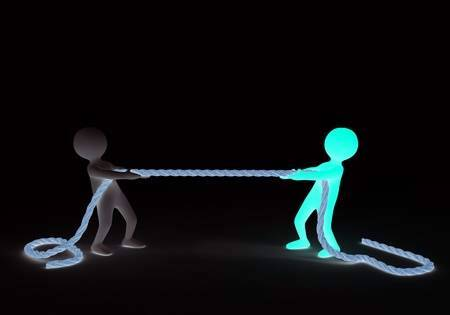
\includegraphics[scale=0.35]{figs/picture-tug-war2-neg.jpg}
      % \includegraphics[scale=0.2]{figs/tug_war.png}
      \vfill
      \begin{tabular}{ c c c  }
        $\Delta u$ &  & $\dot{W} u$ \\ [0.5em] \hline \\
        Smoothing  &  & Roughening  \\
      \end{tabular}
   \end{center}
\end{frame}
\begin{frame} % Propagation of tall peaks
  \begin{center}
    $\dfrac{\partial}{\partial t} u(t,x) = \left(\dfrac{1}{2}\dfrac{\partial^2}{\partial x^2} + \lambda \dot{W}(t,x)\right)u(t,x)$ \\[0.5em] \small
     --- Propagation of tall peaks \footnote{\textcolor{refcolor}{C. \& Dalang}, {\it Ann. of Prob.}, 43 (6), (2015).}
  \end{center}
  \small
  \vfill \bigskip

  \centering
  \only<2-7>{
    \visible<2-7>{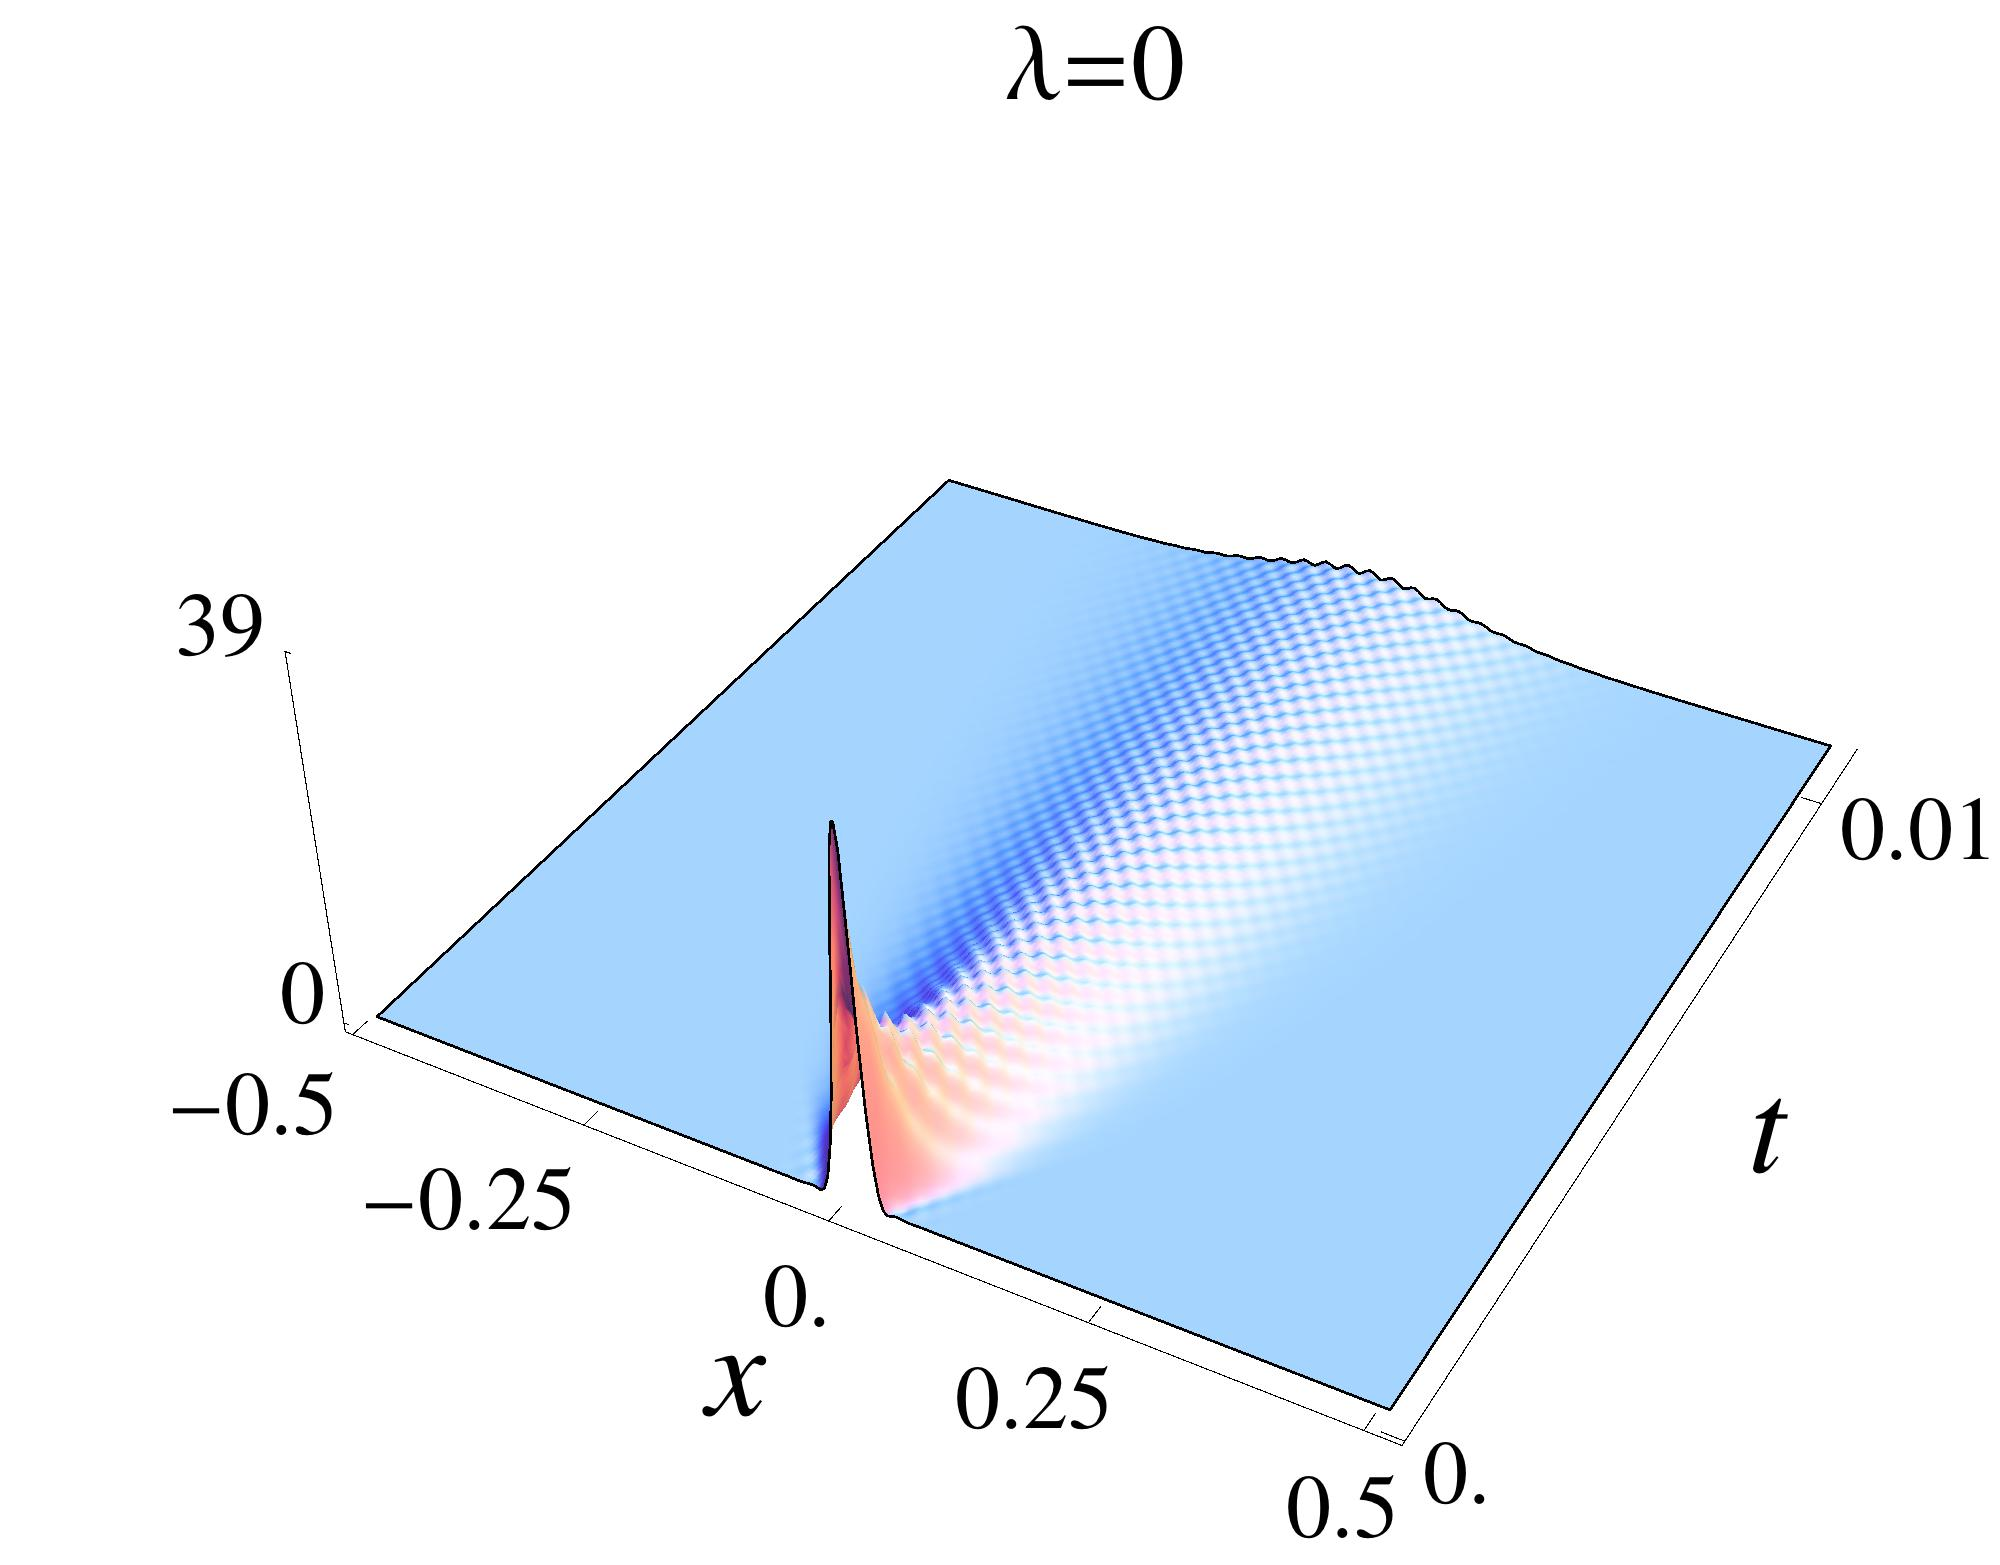
\includegraphics[scale=0.05]{figs/small_Delta_L0.jpeg}}
    \visible<3-7>{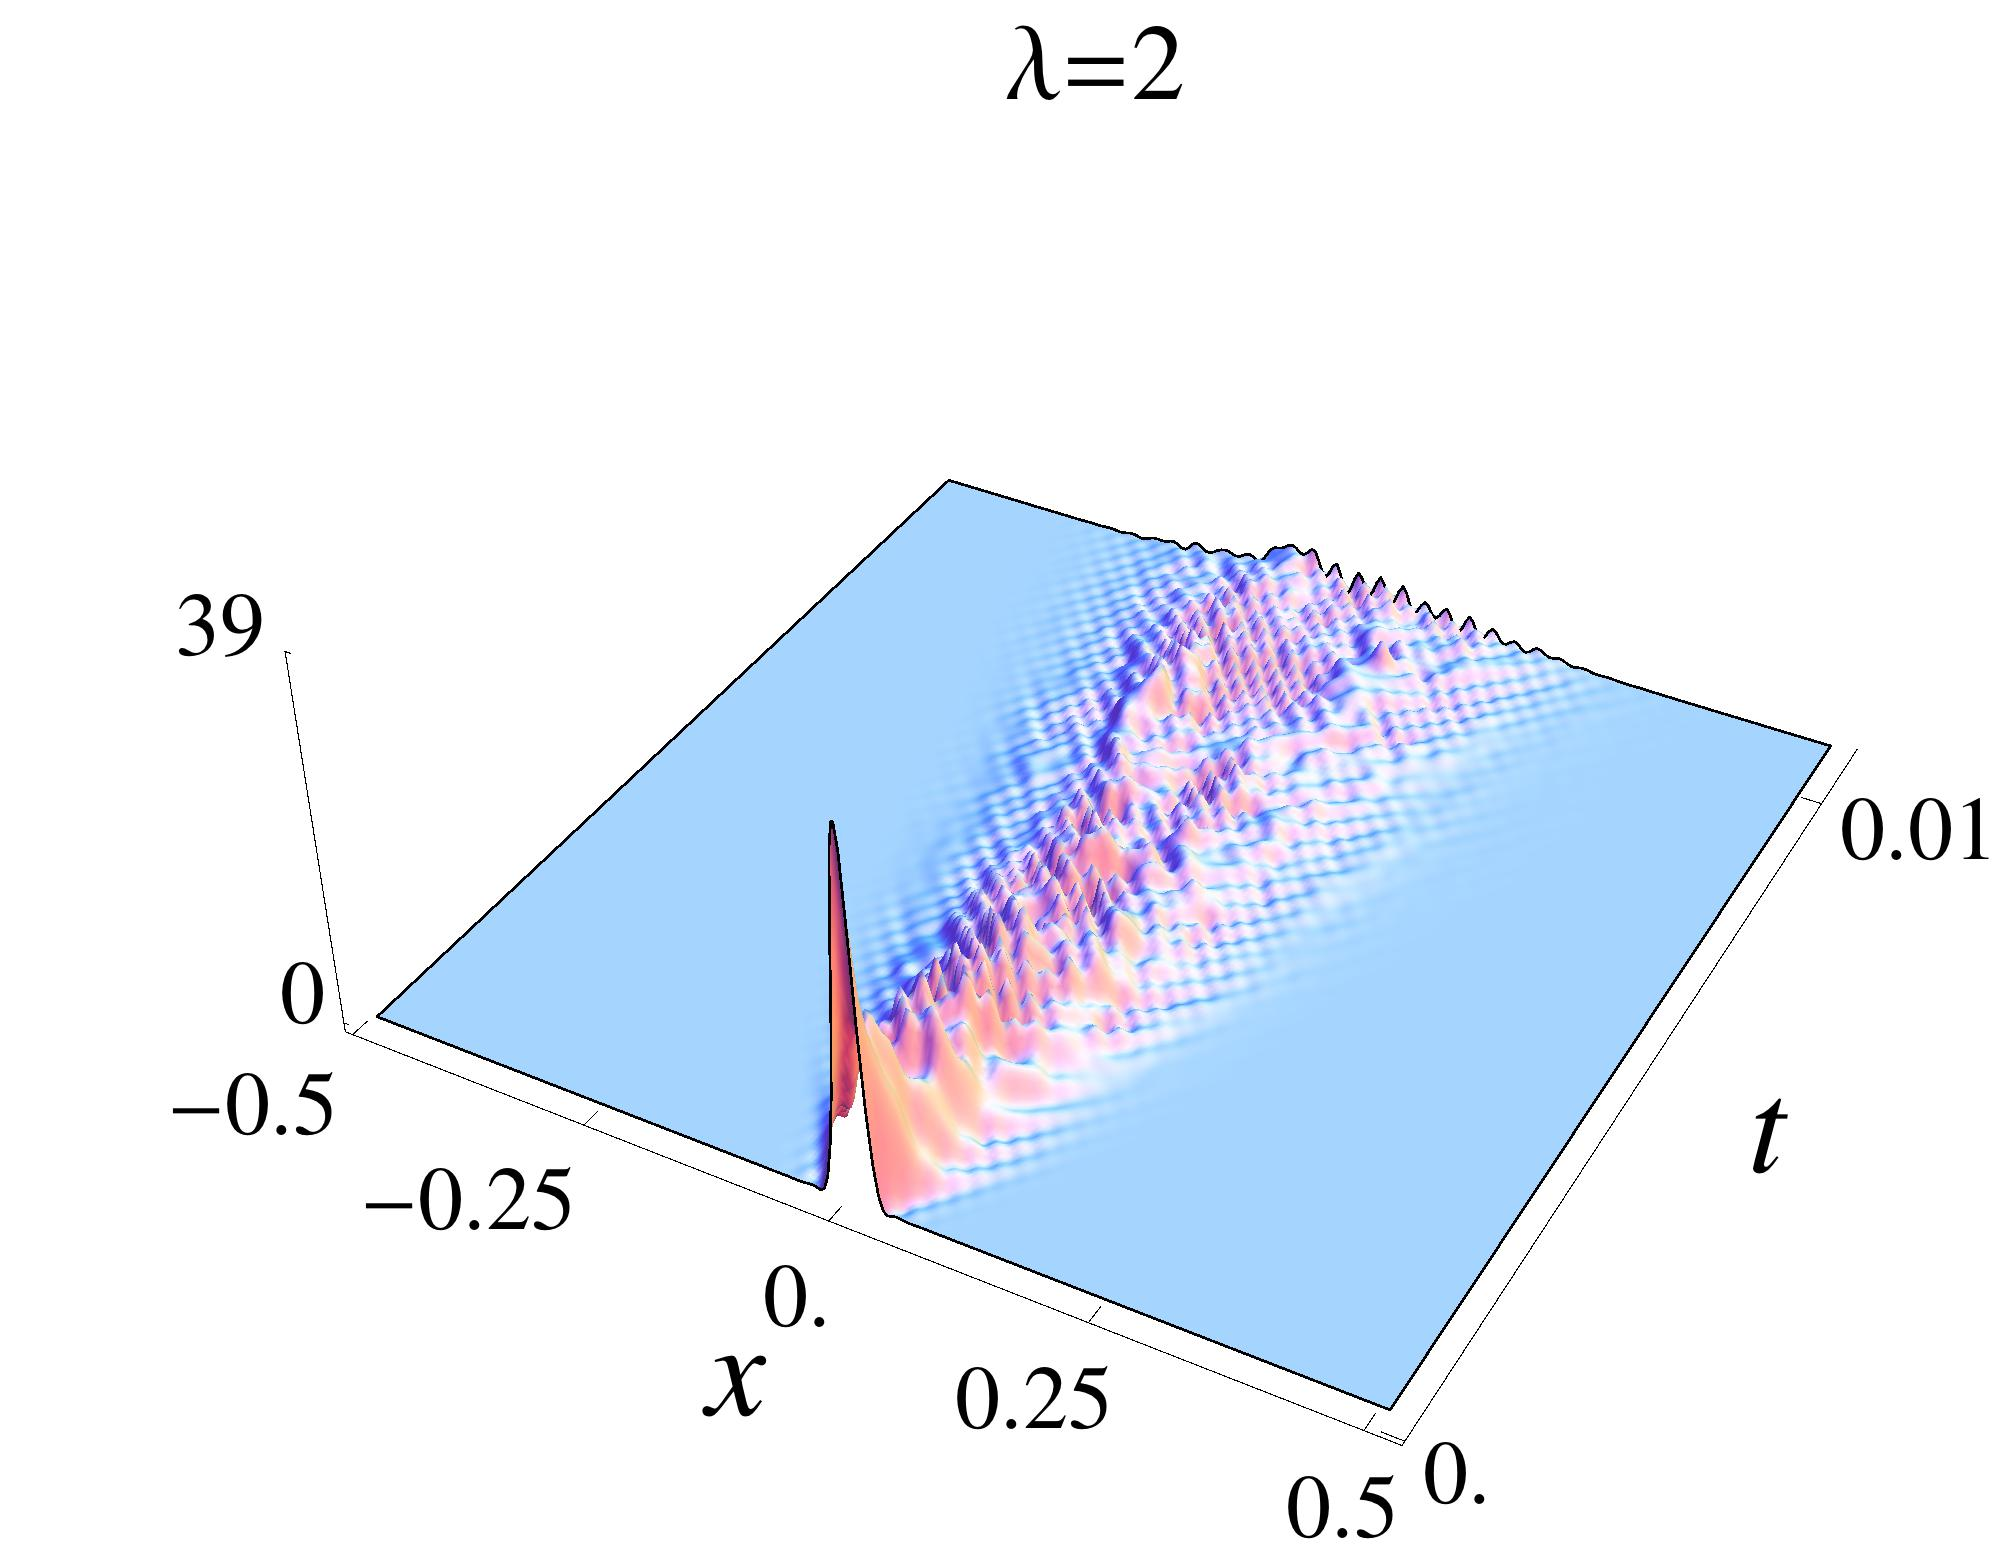
\includegraphics[scale=0.05]{figs/small_Delta_L2.jpeg}}
    \visible<4-7>{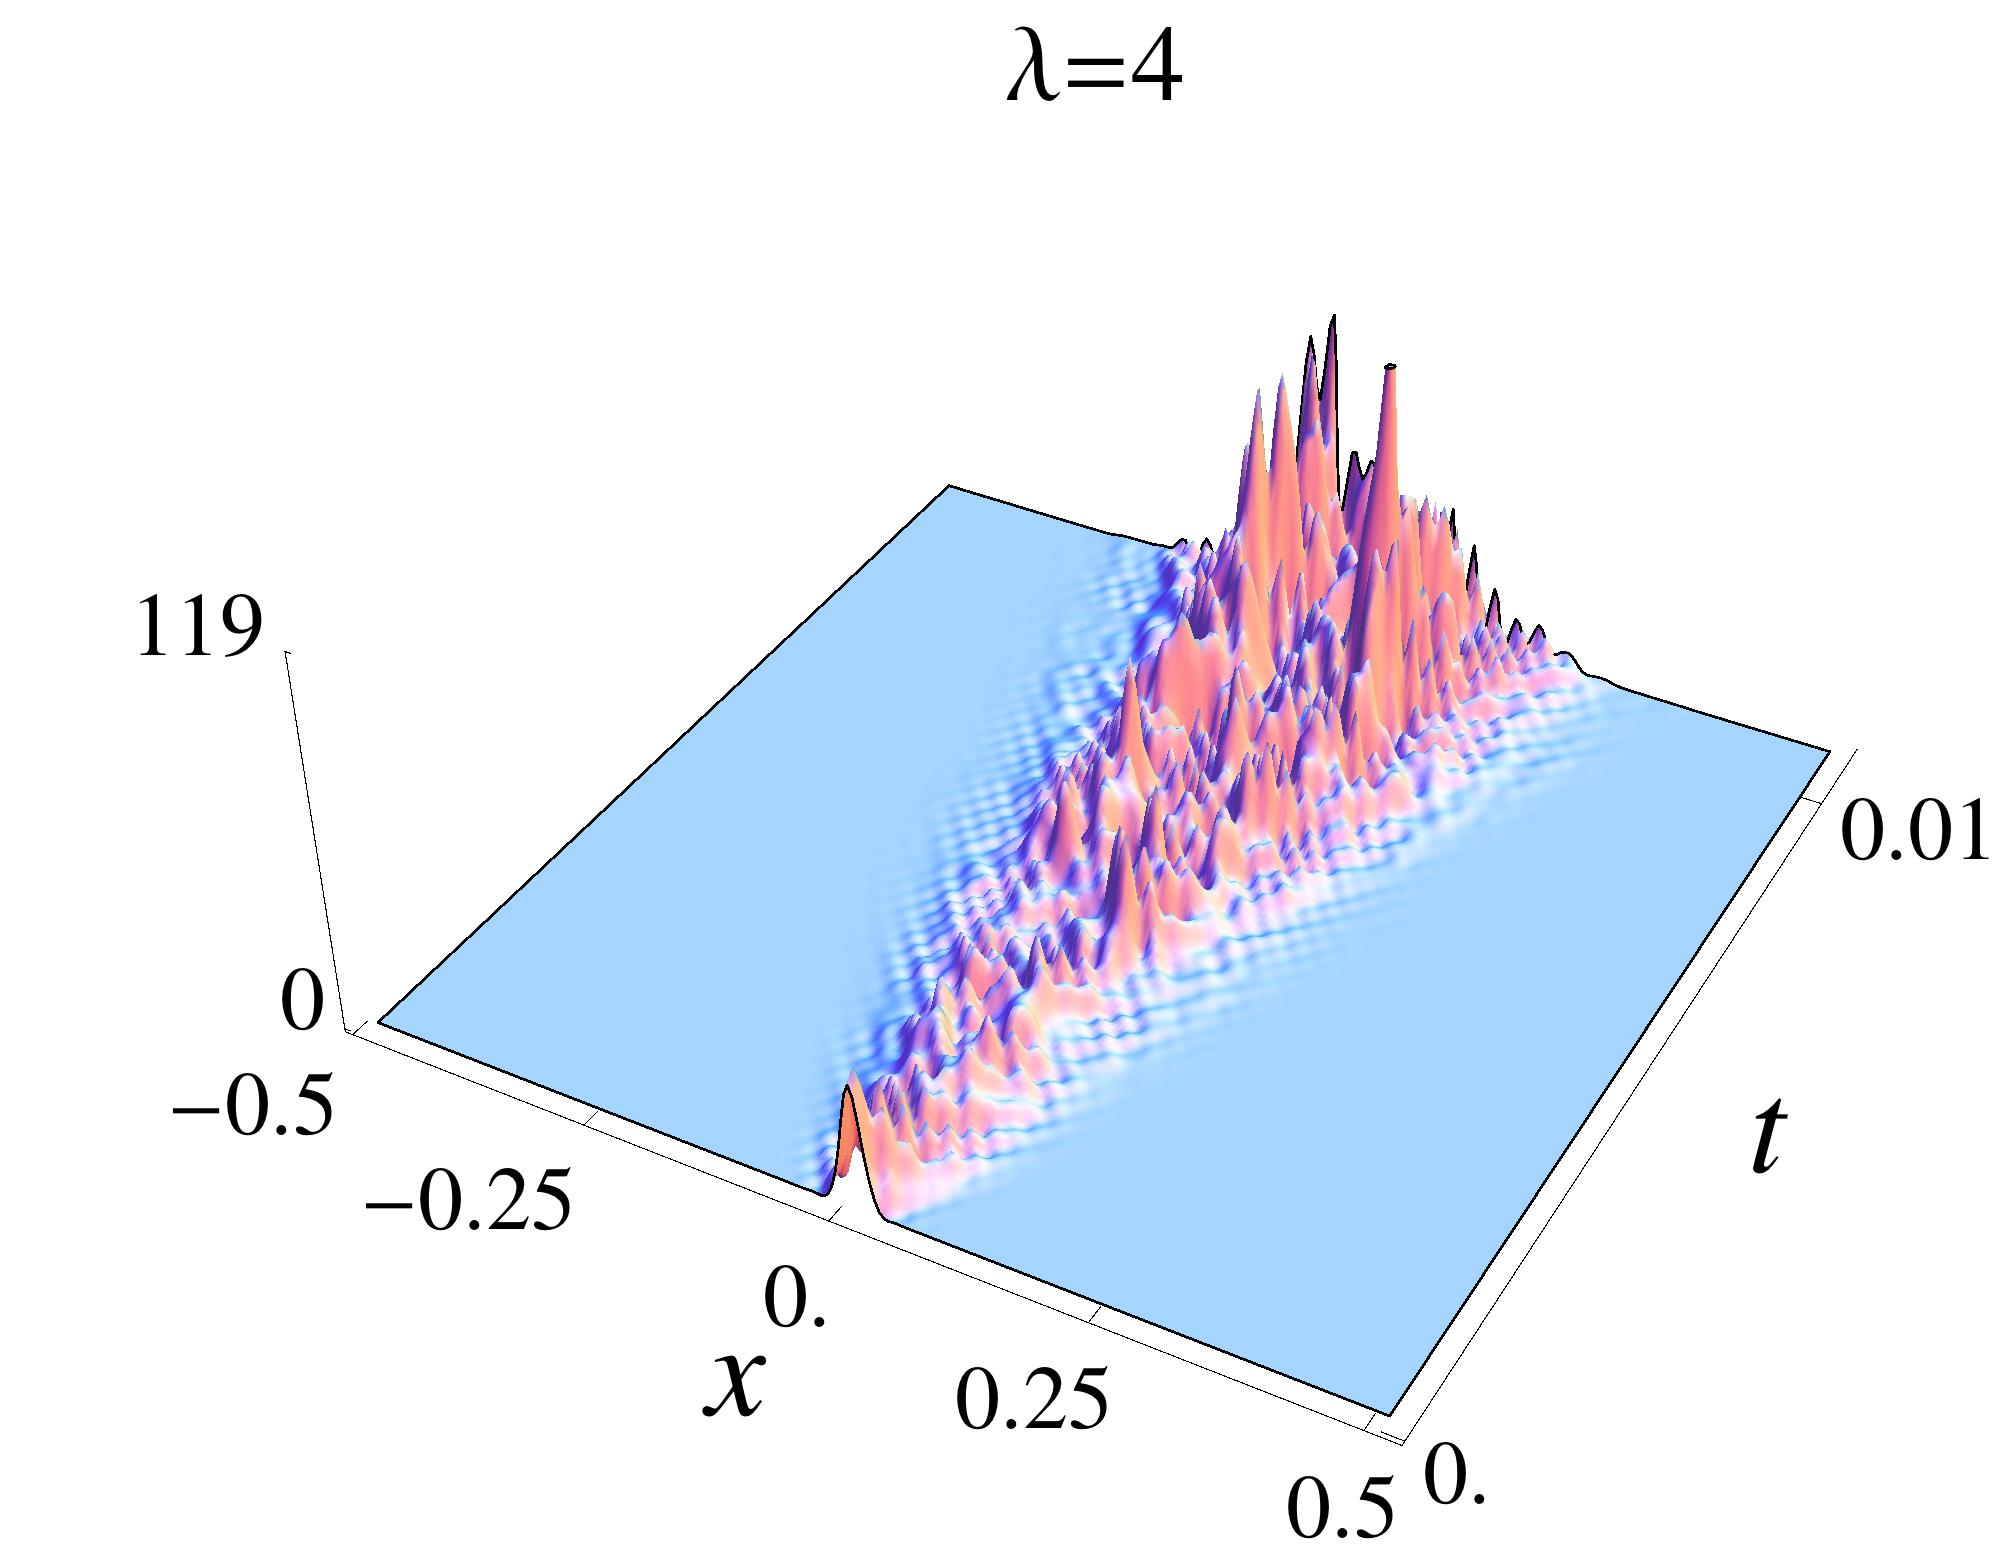
\includegraphics[scale=0.05]{figs/small_Delta_L4.jpeg}}\\ \vfill
    \visible<5-7>{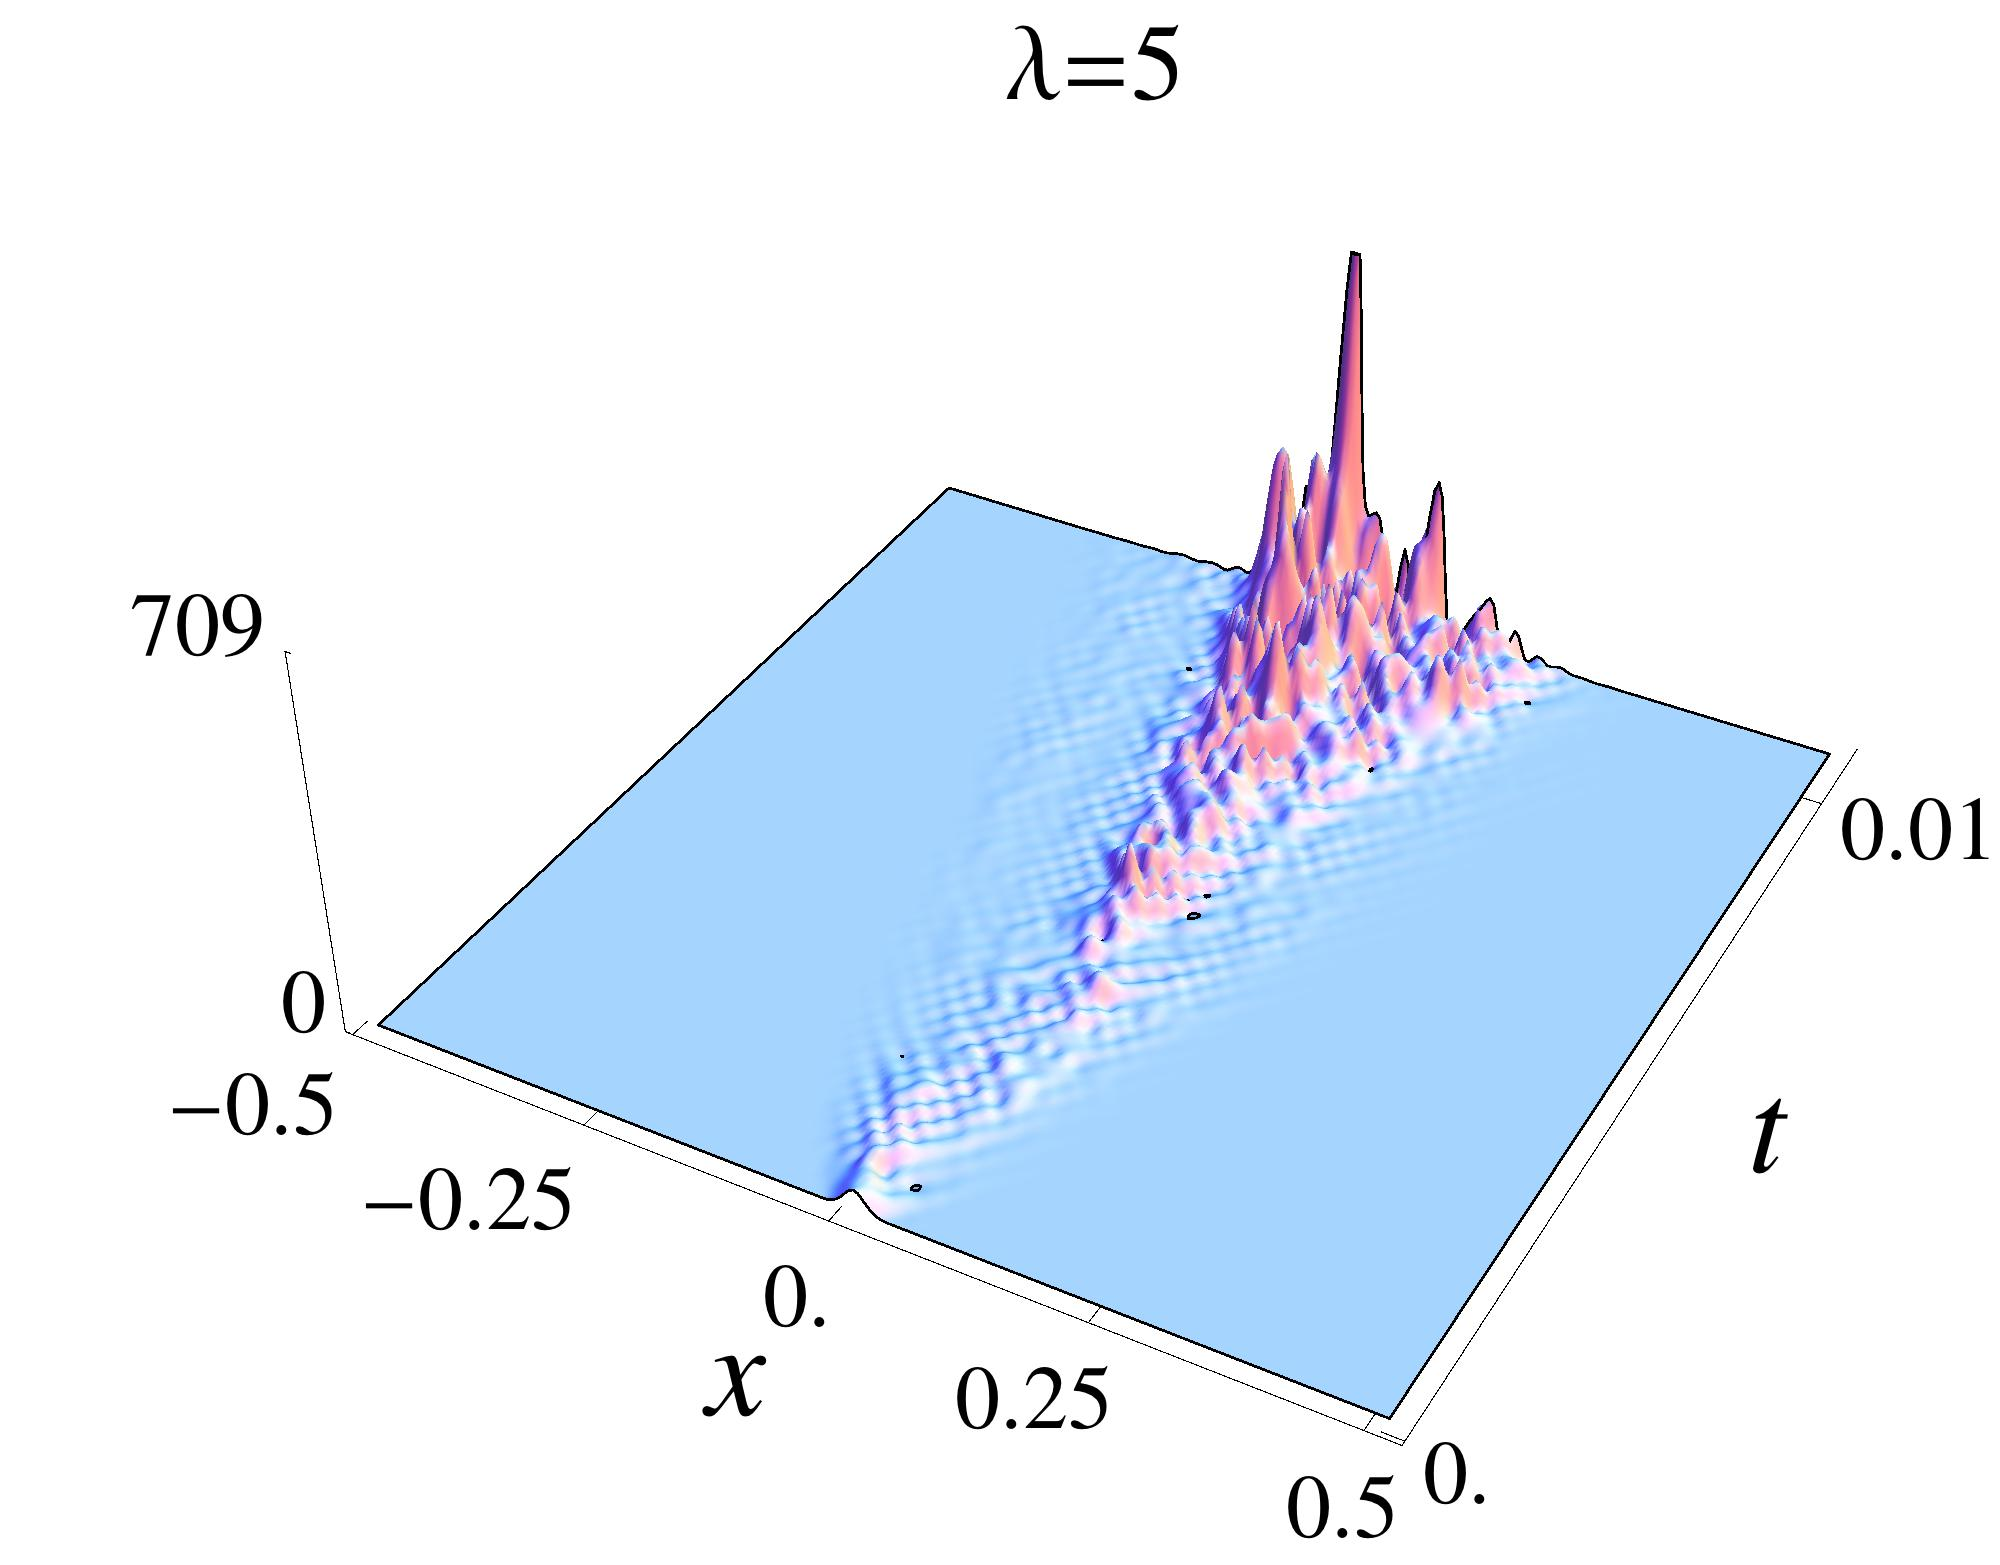
\includegraphics[scale=0.05]{figs/small_Delta_L5.jpeg}}
    \visible<6-7>{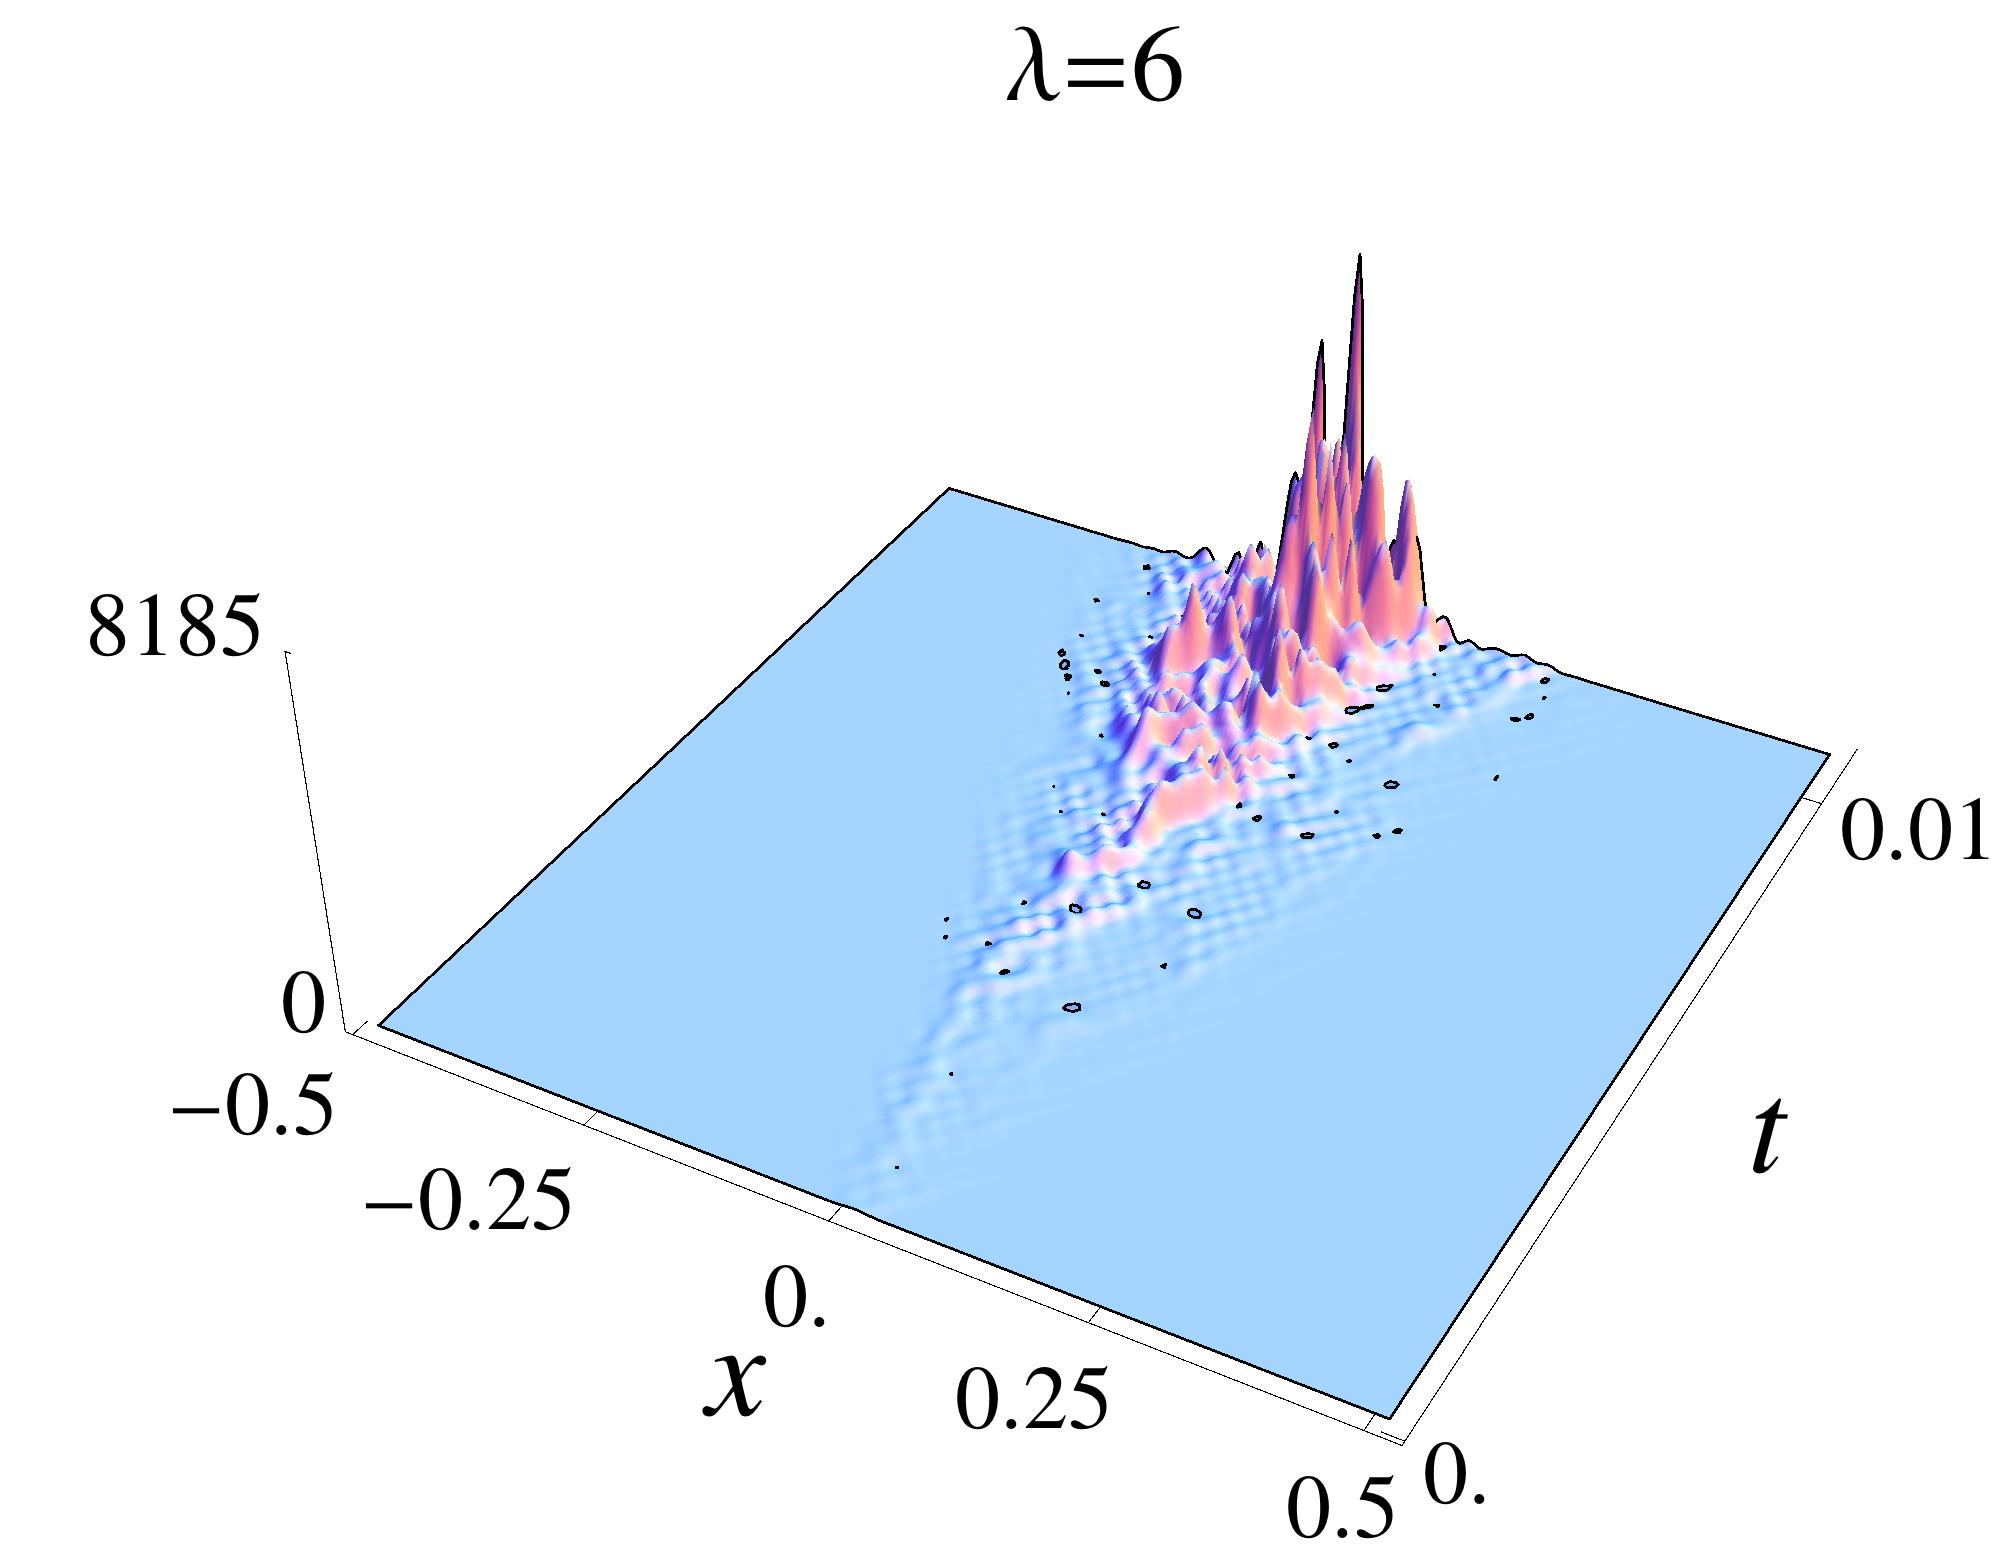
\includegraphics[scale=0.05]{figs/small_Delta_L6.jpeg}}
    \visible<7>{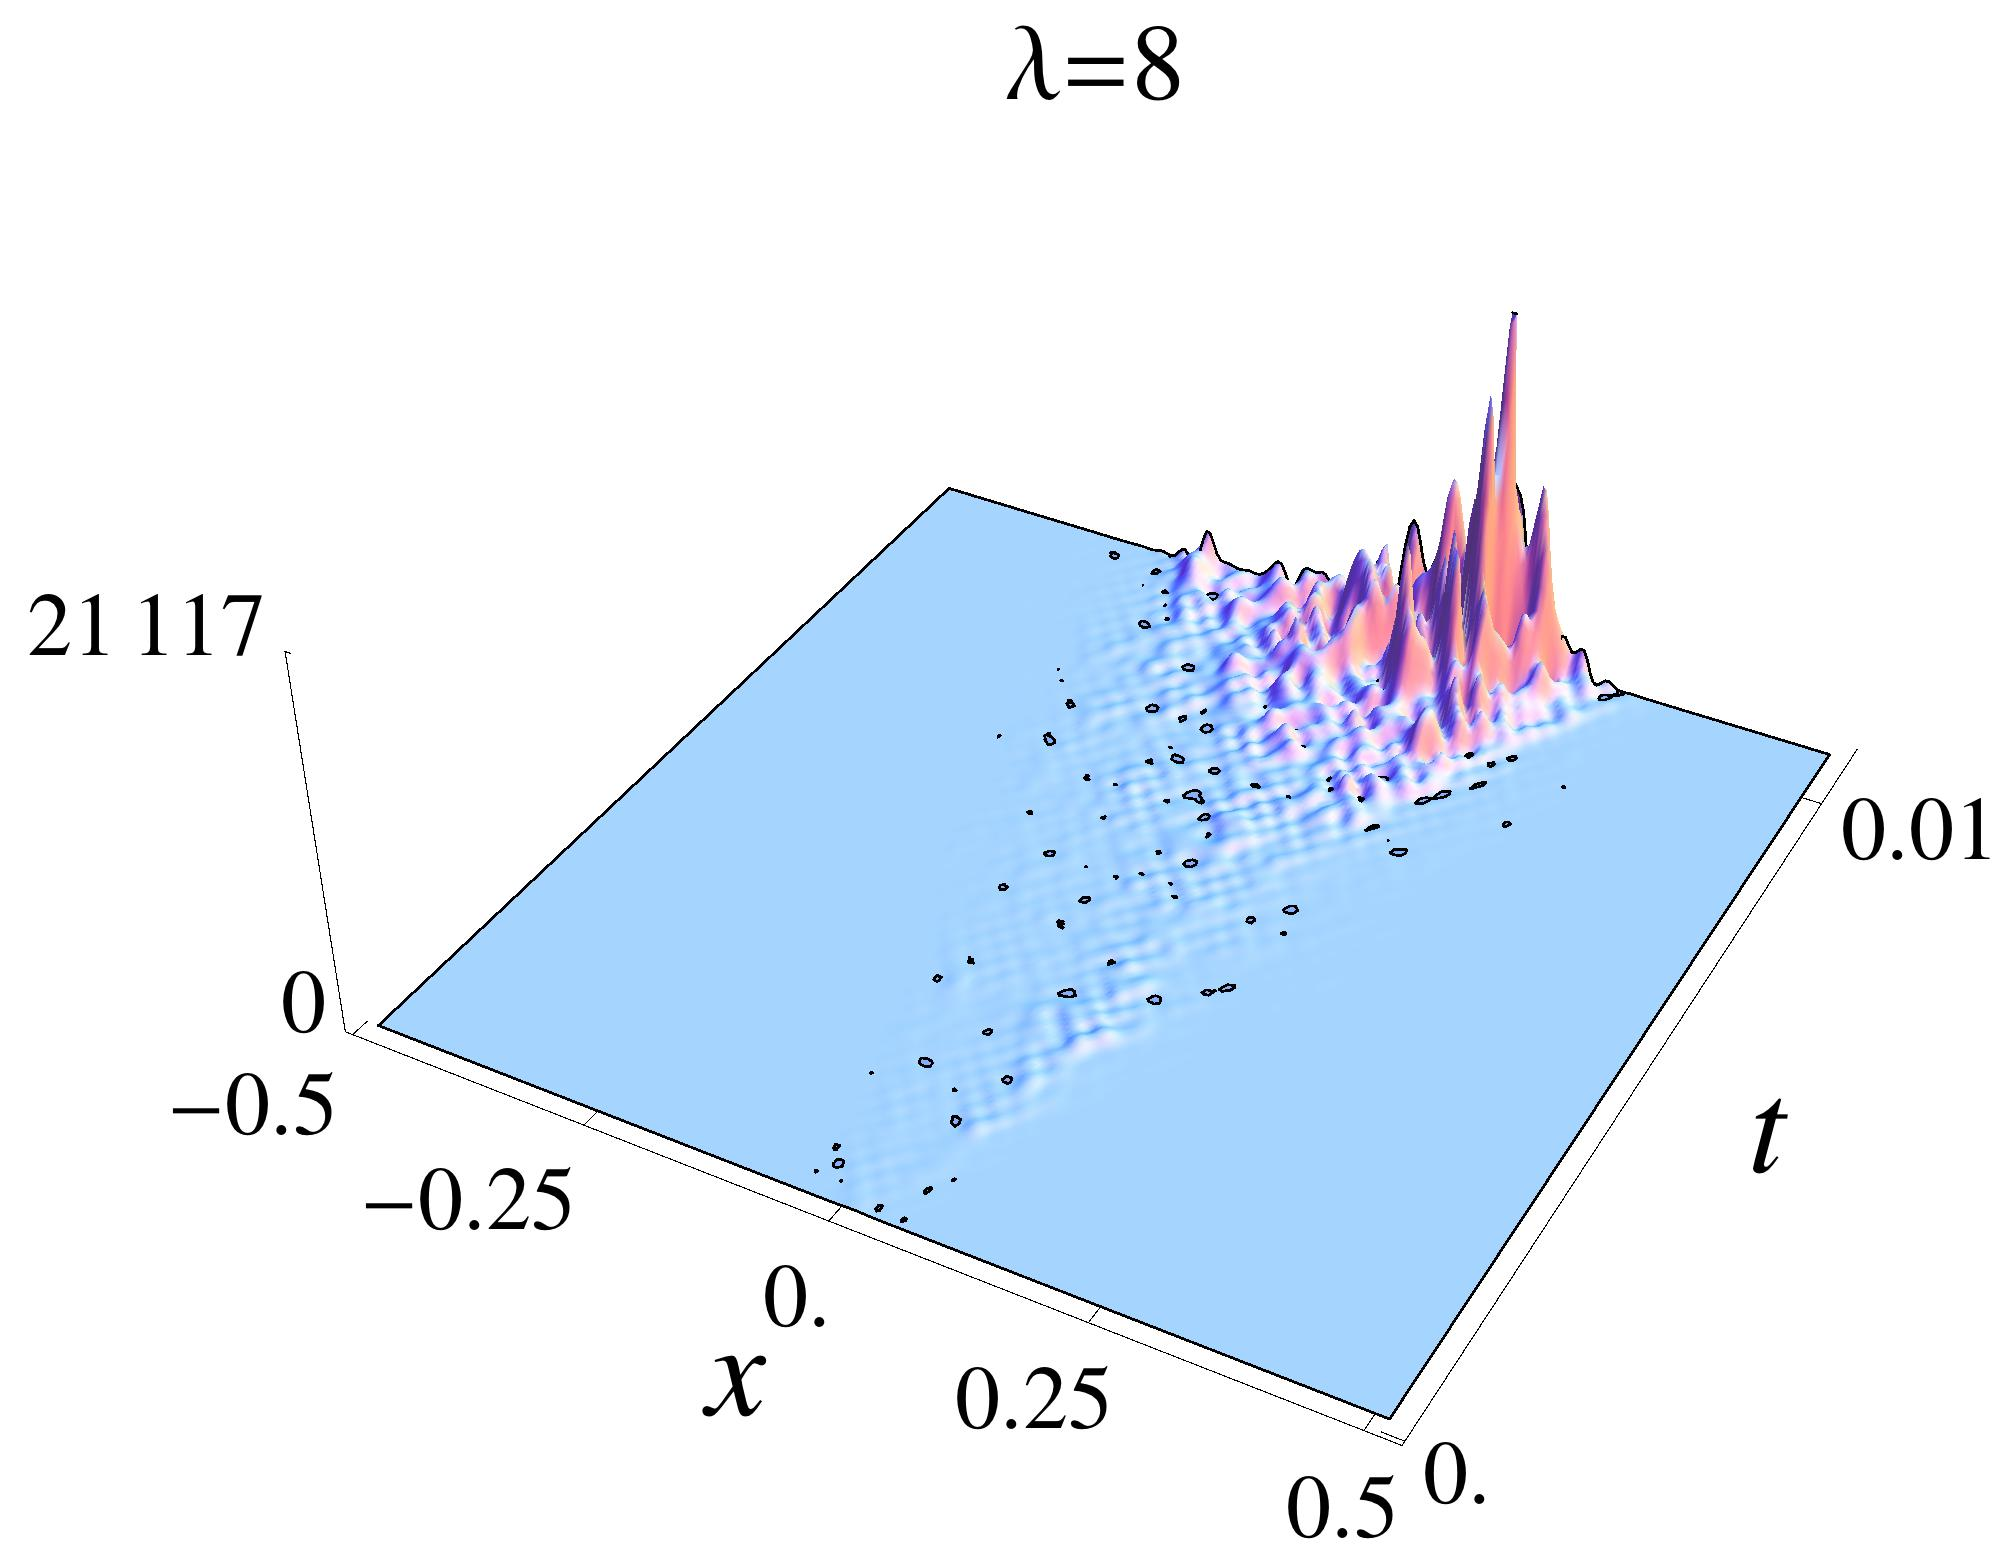
\includegraphics[scale=0.05]{figs/small_Delta_L8.jpeg}}\\
    \phantom{aaa}\\[3.3em]
    \phantom{aaaaaa}
    }
  \only<8->{
    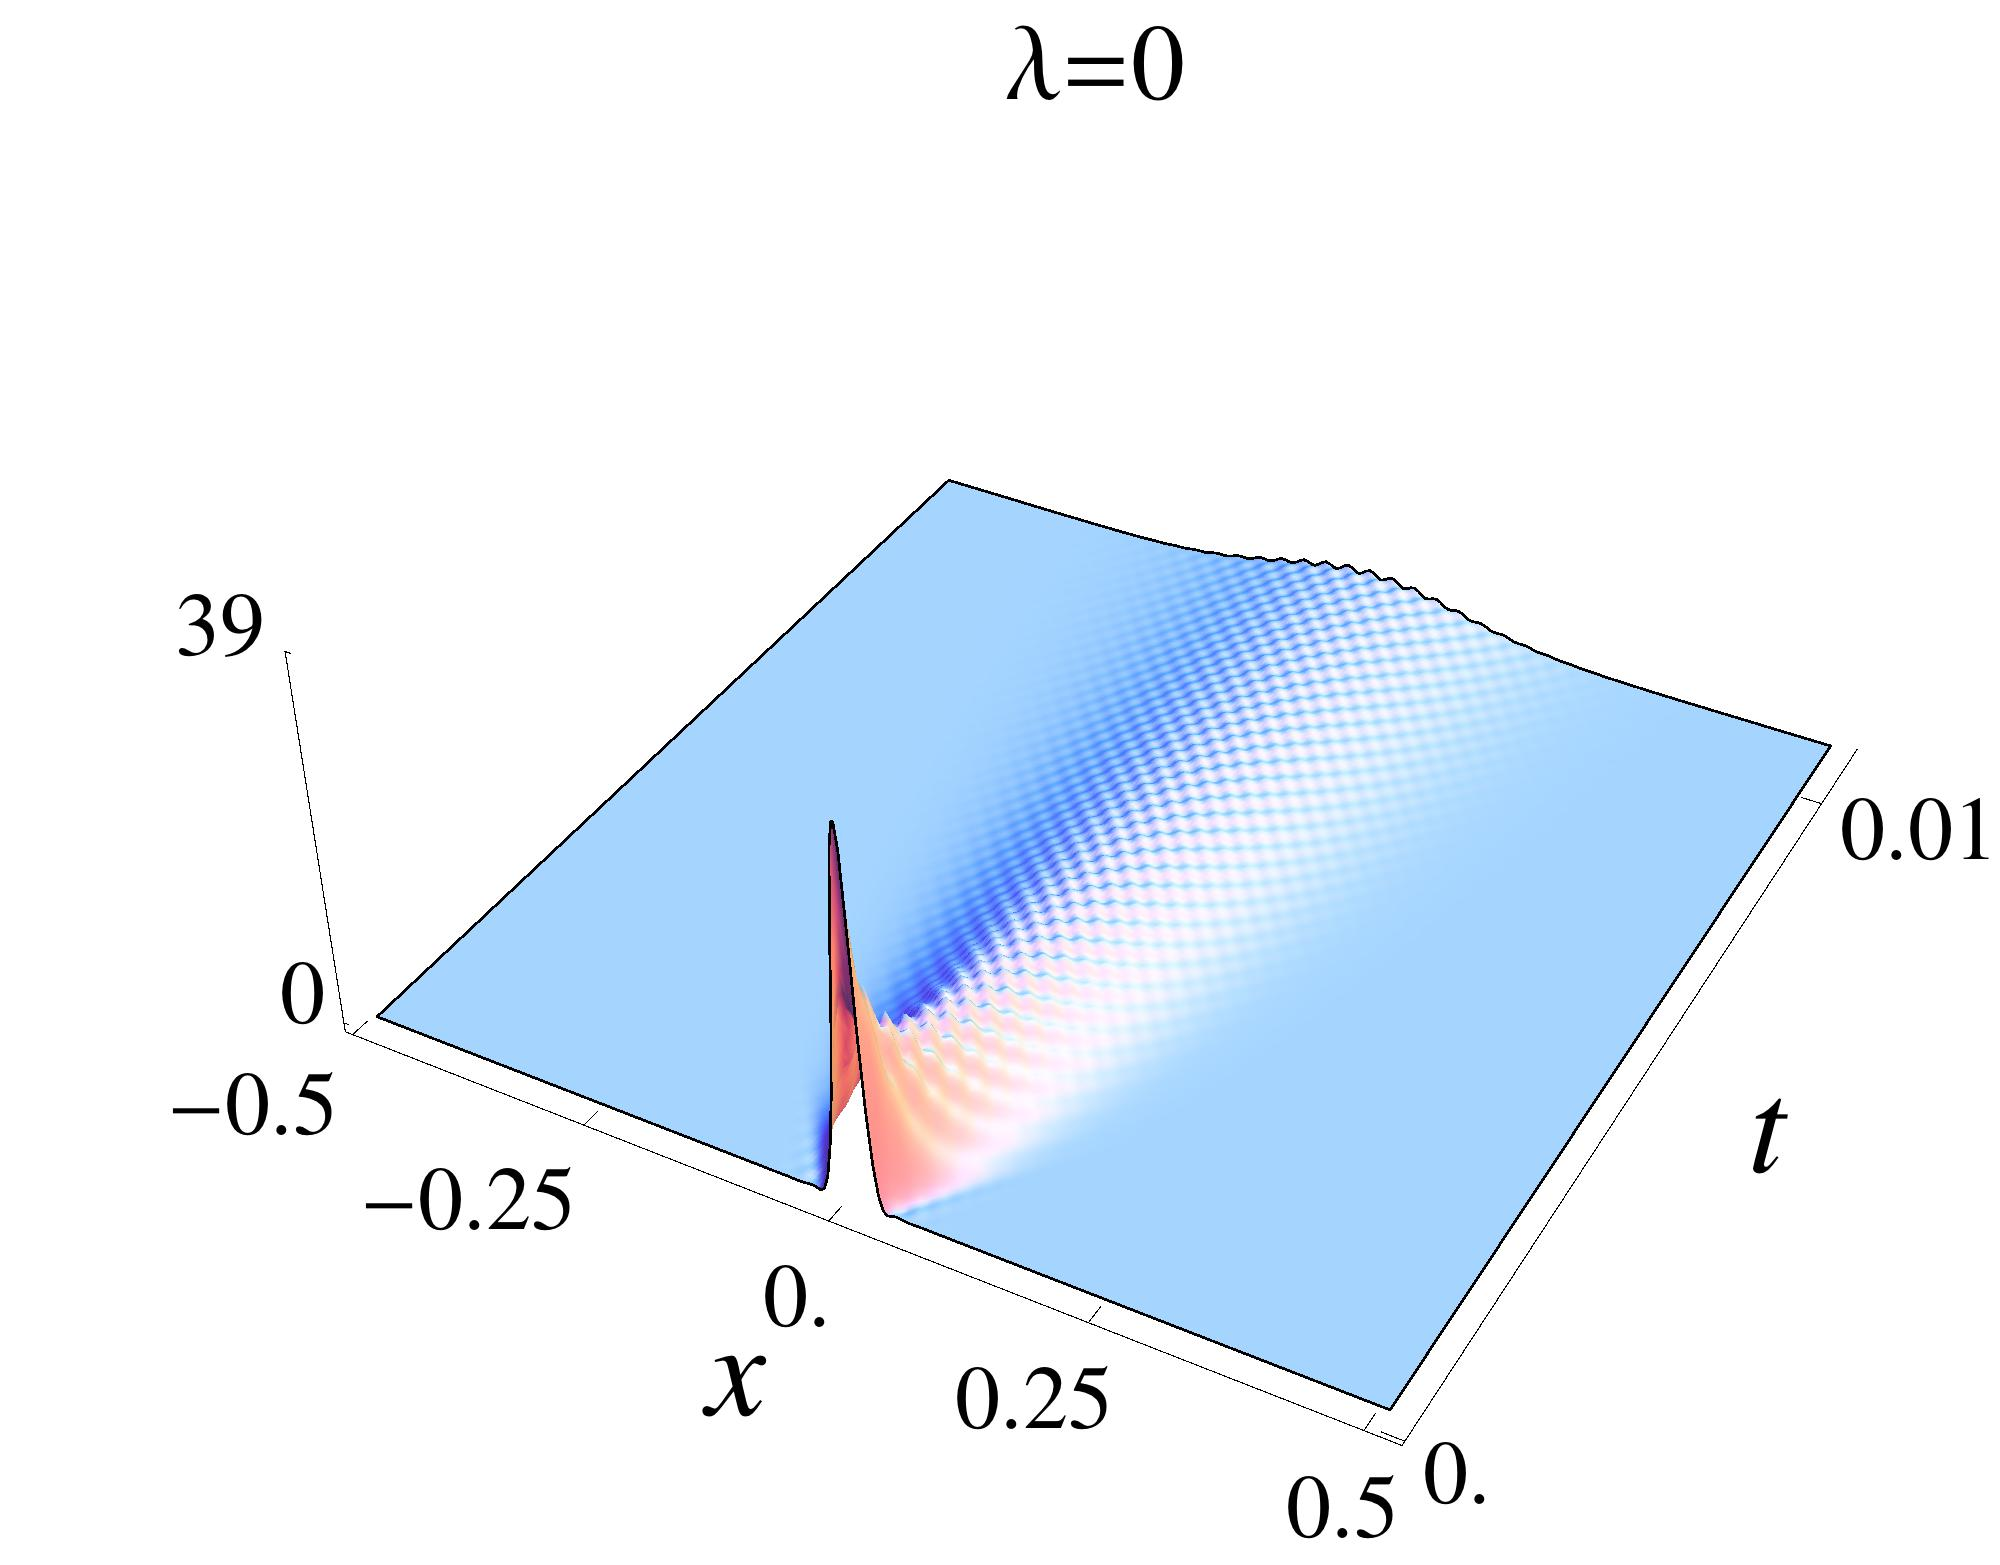
\includegraphics[scale=0.05]{figs/small_Delta_L0_cut.jpeg}
    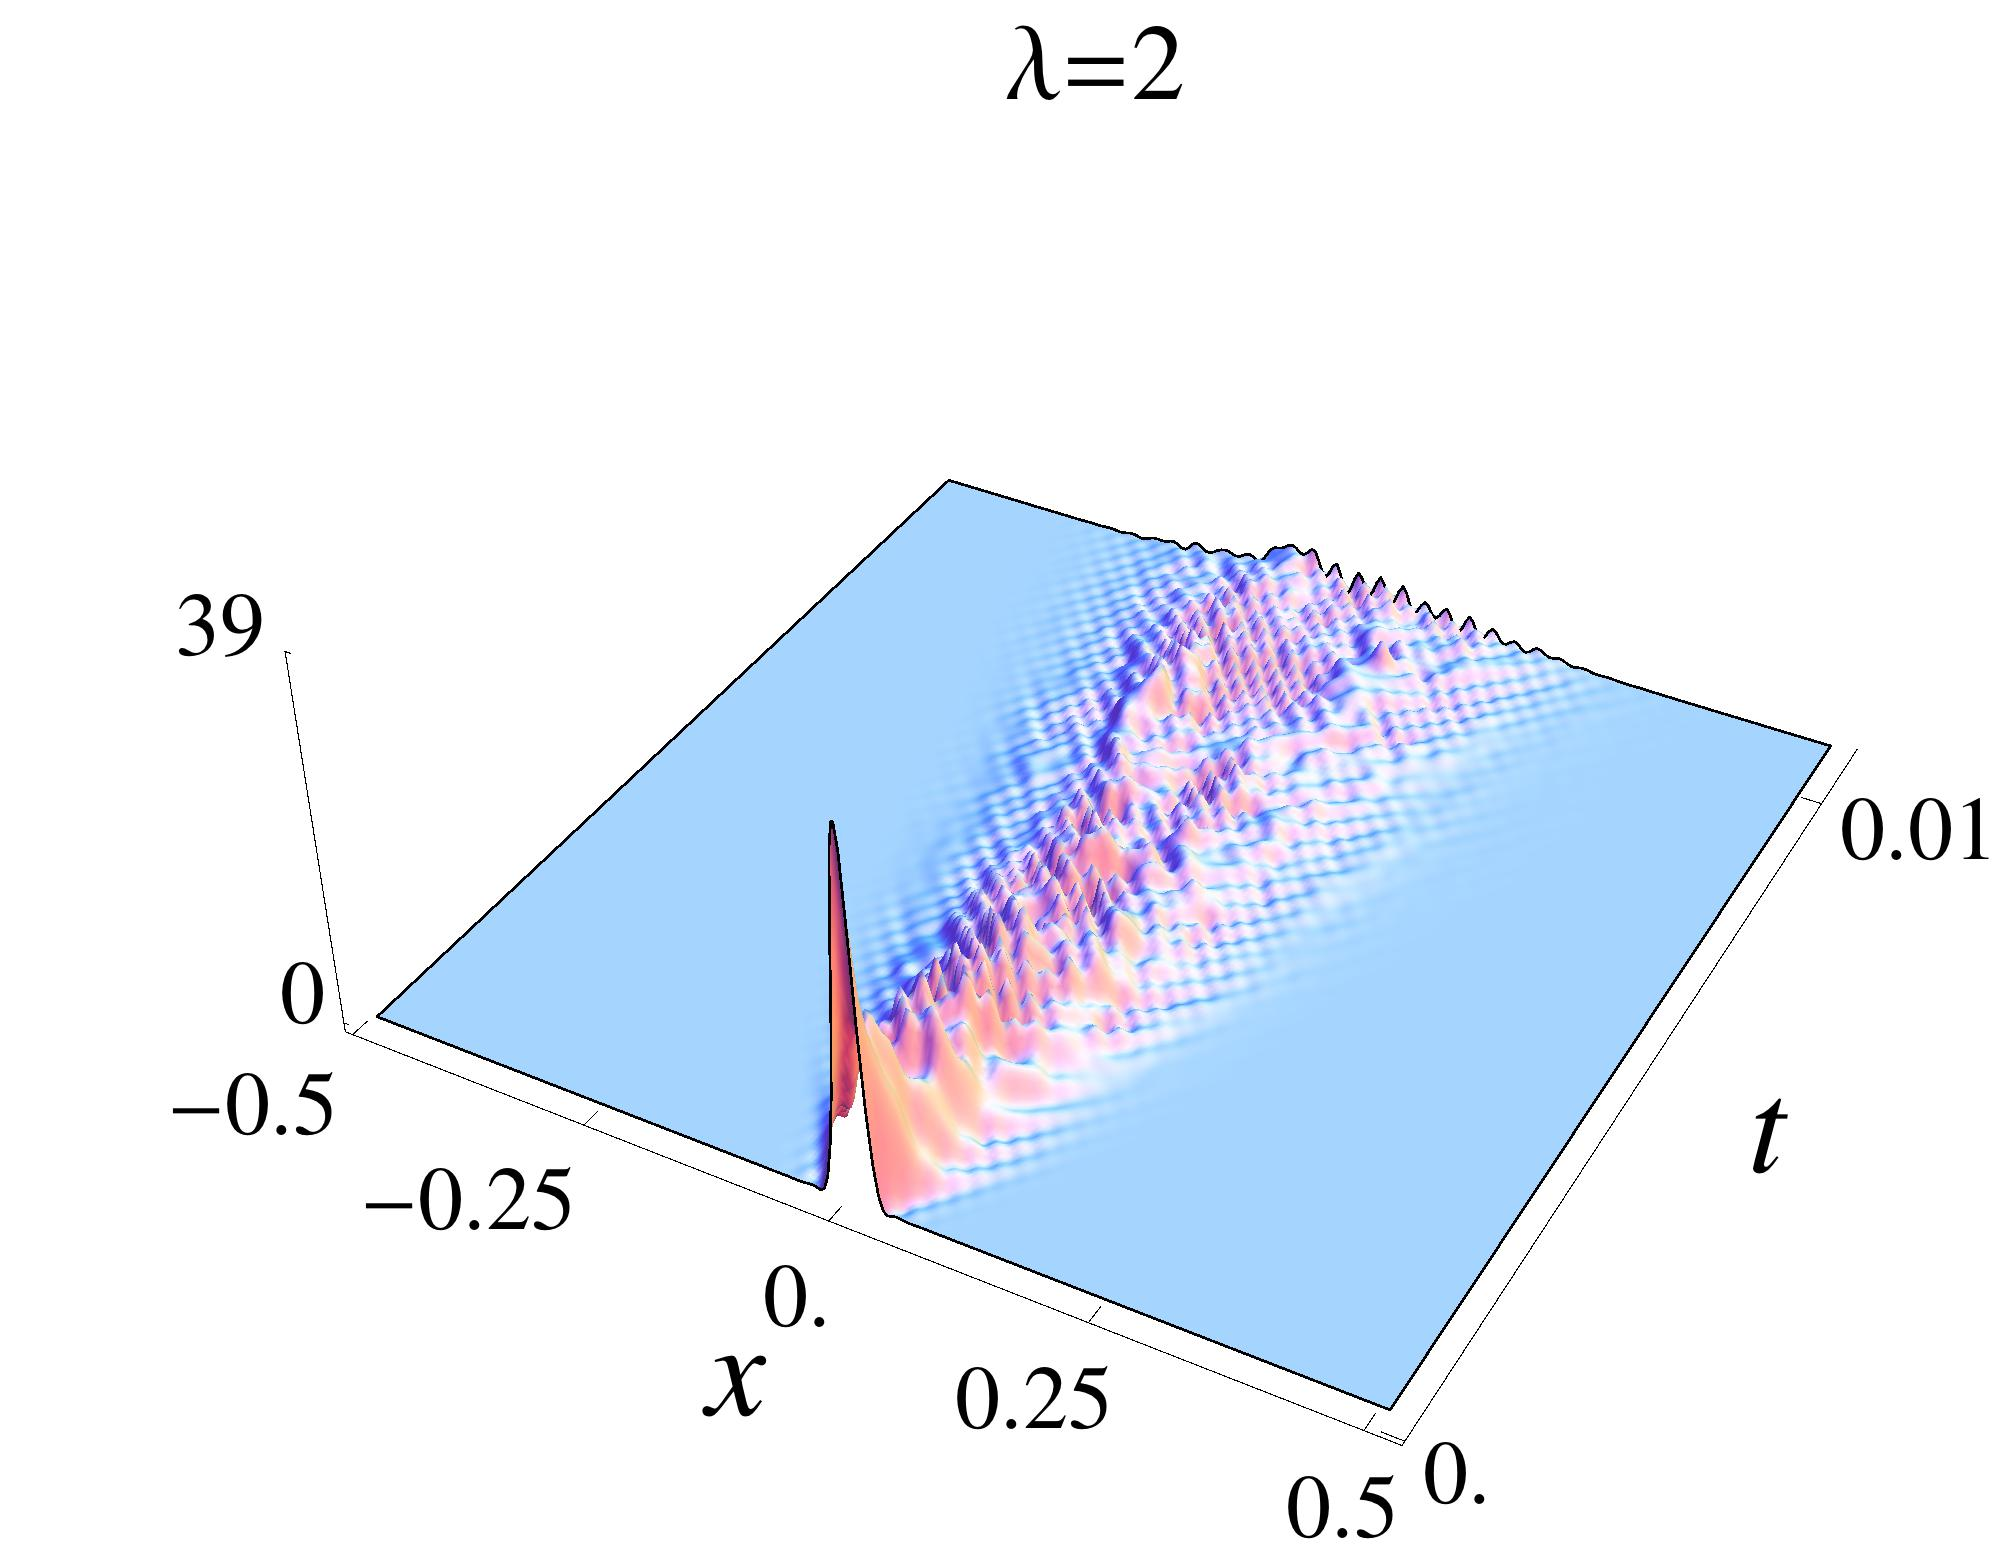
\includegraphics[scale=0.05]{figs/small_Delta_L2_cut.jpeg}
    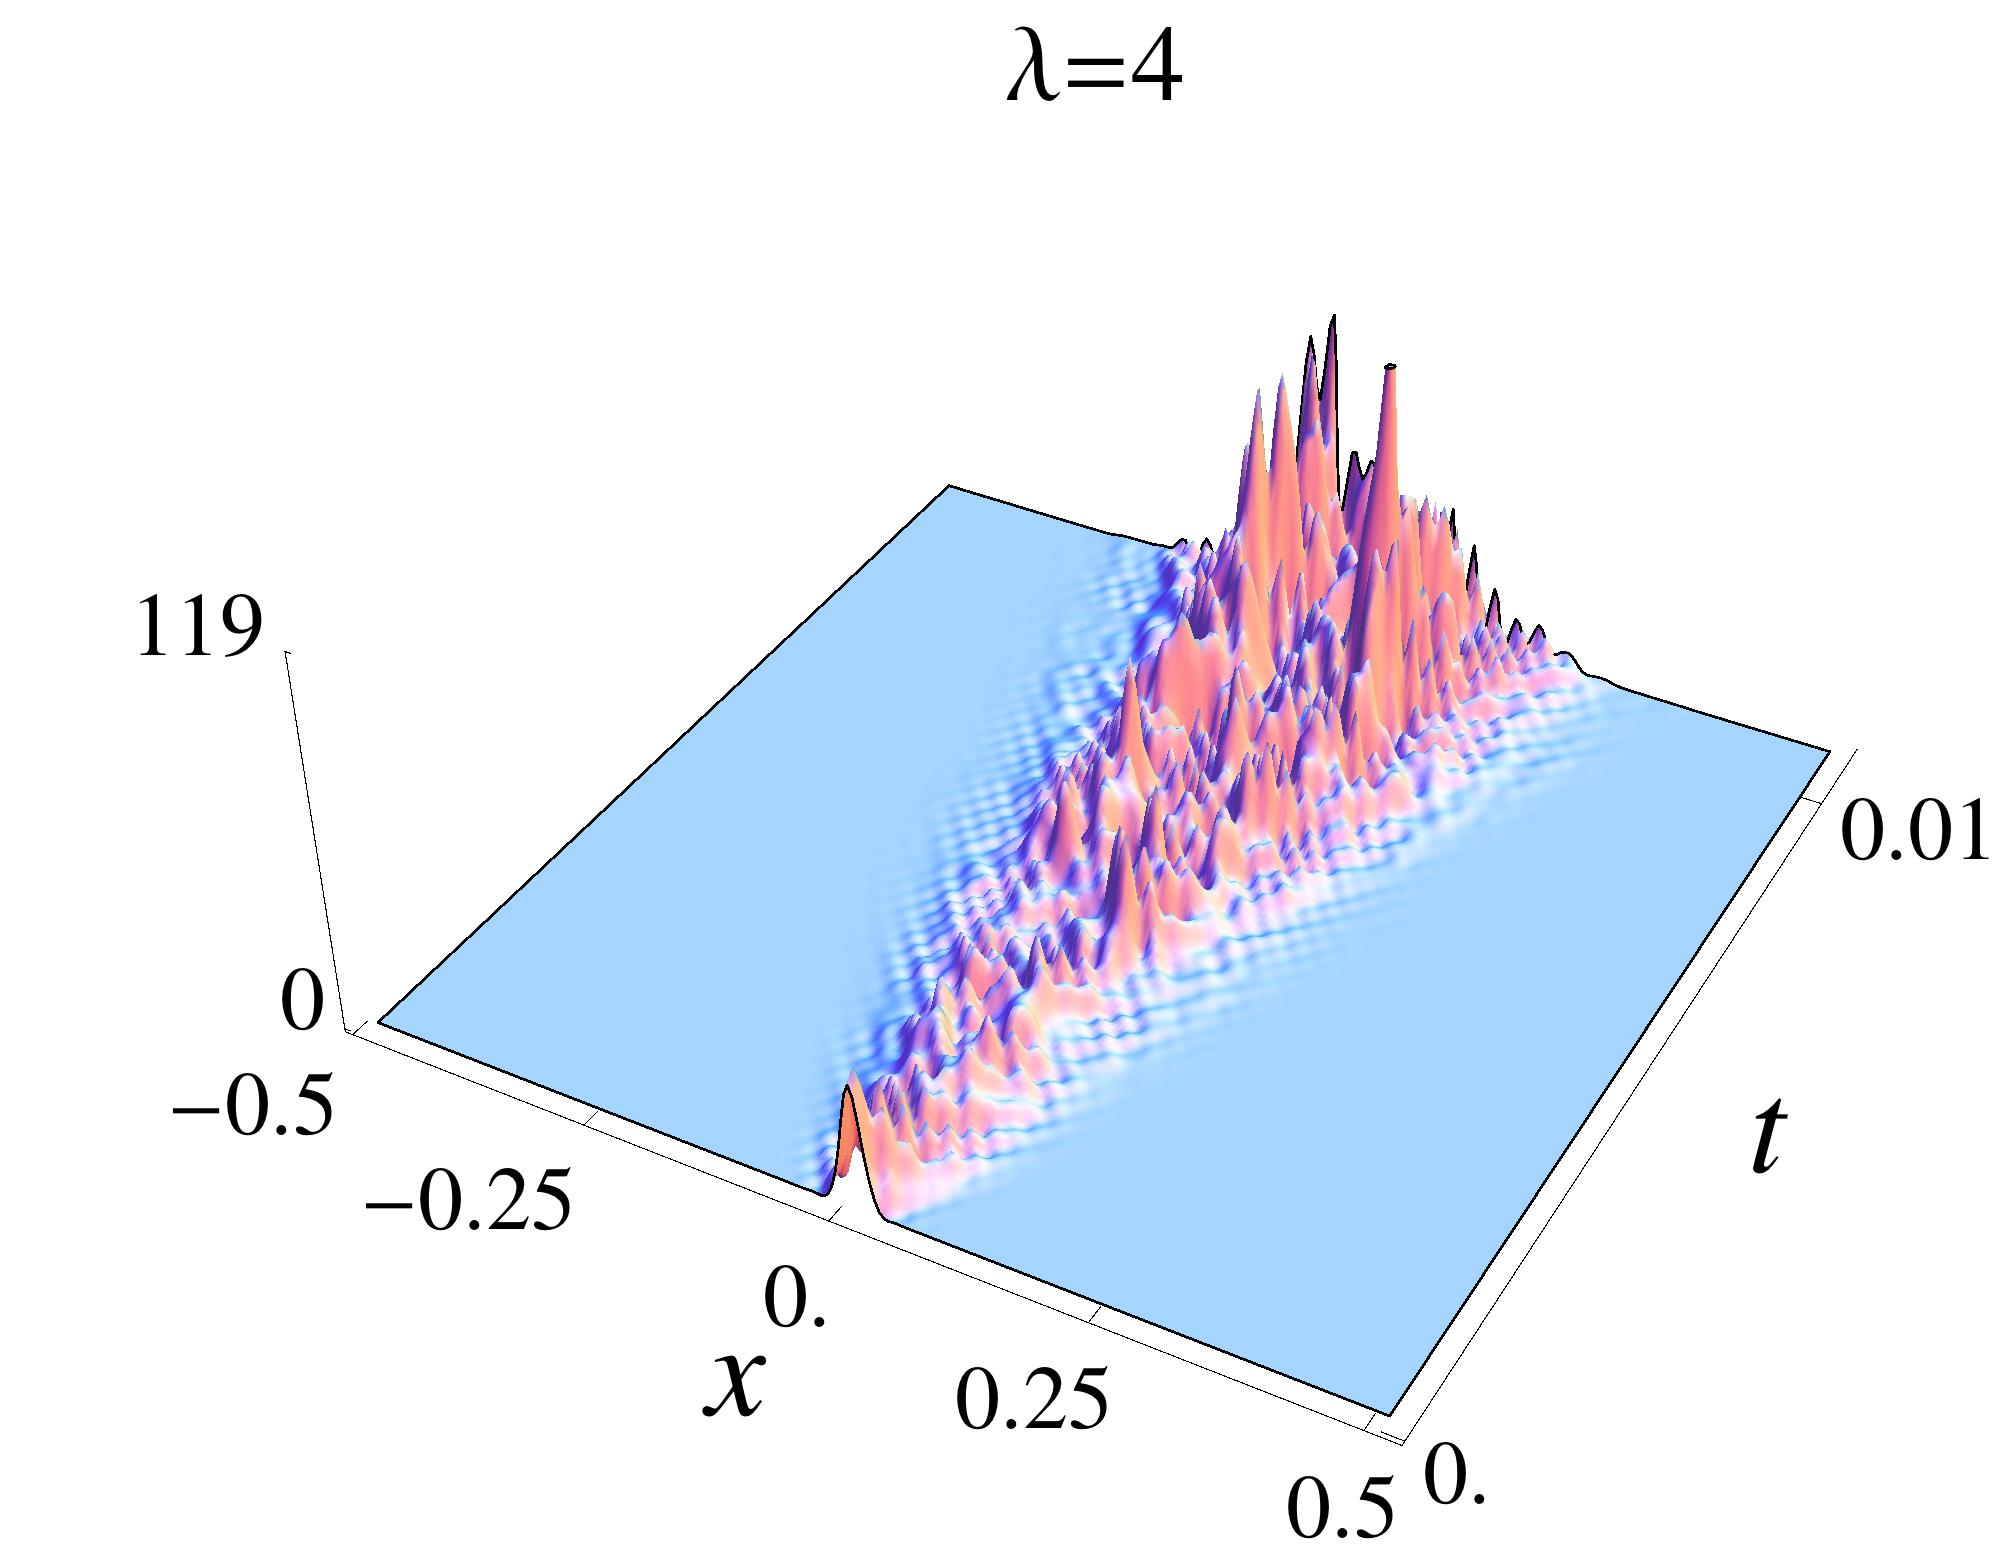
\includegraphics[scale=0.05]{figs/small_Delta_L4_cut.jpeg}\\ \vfill
    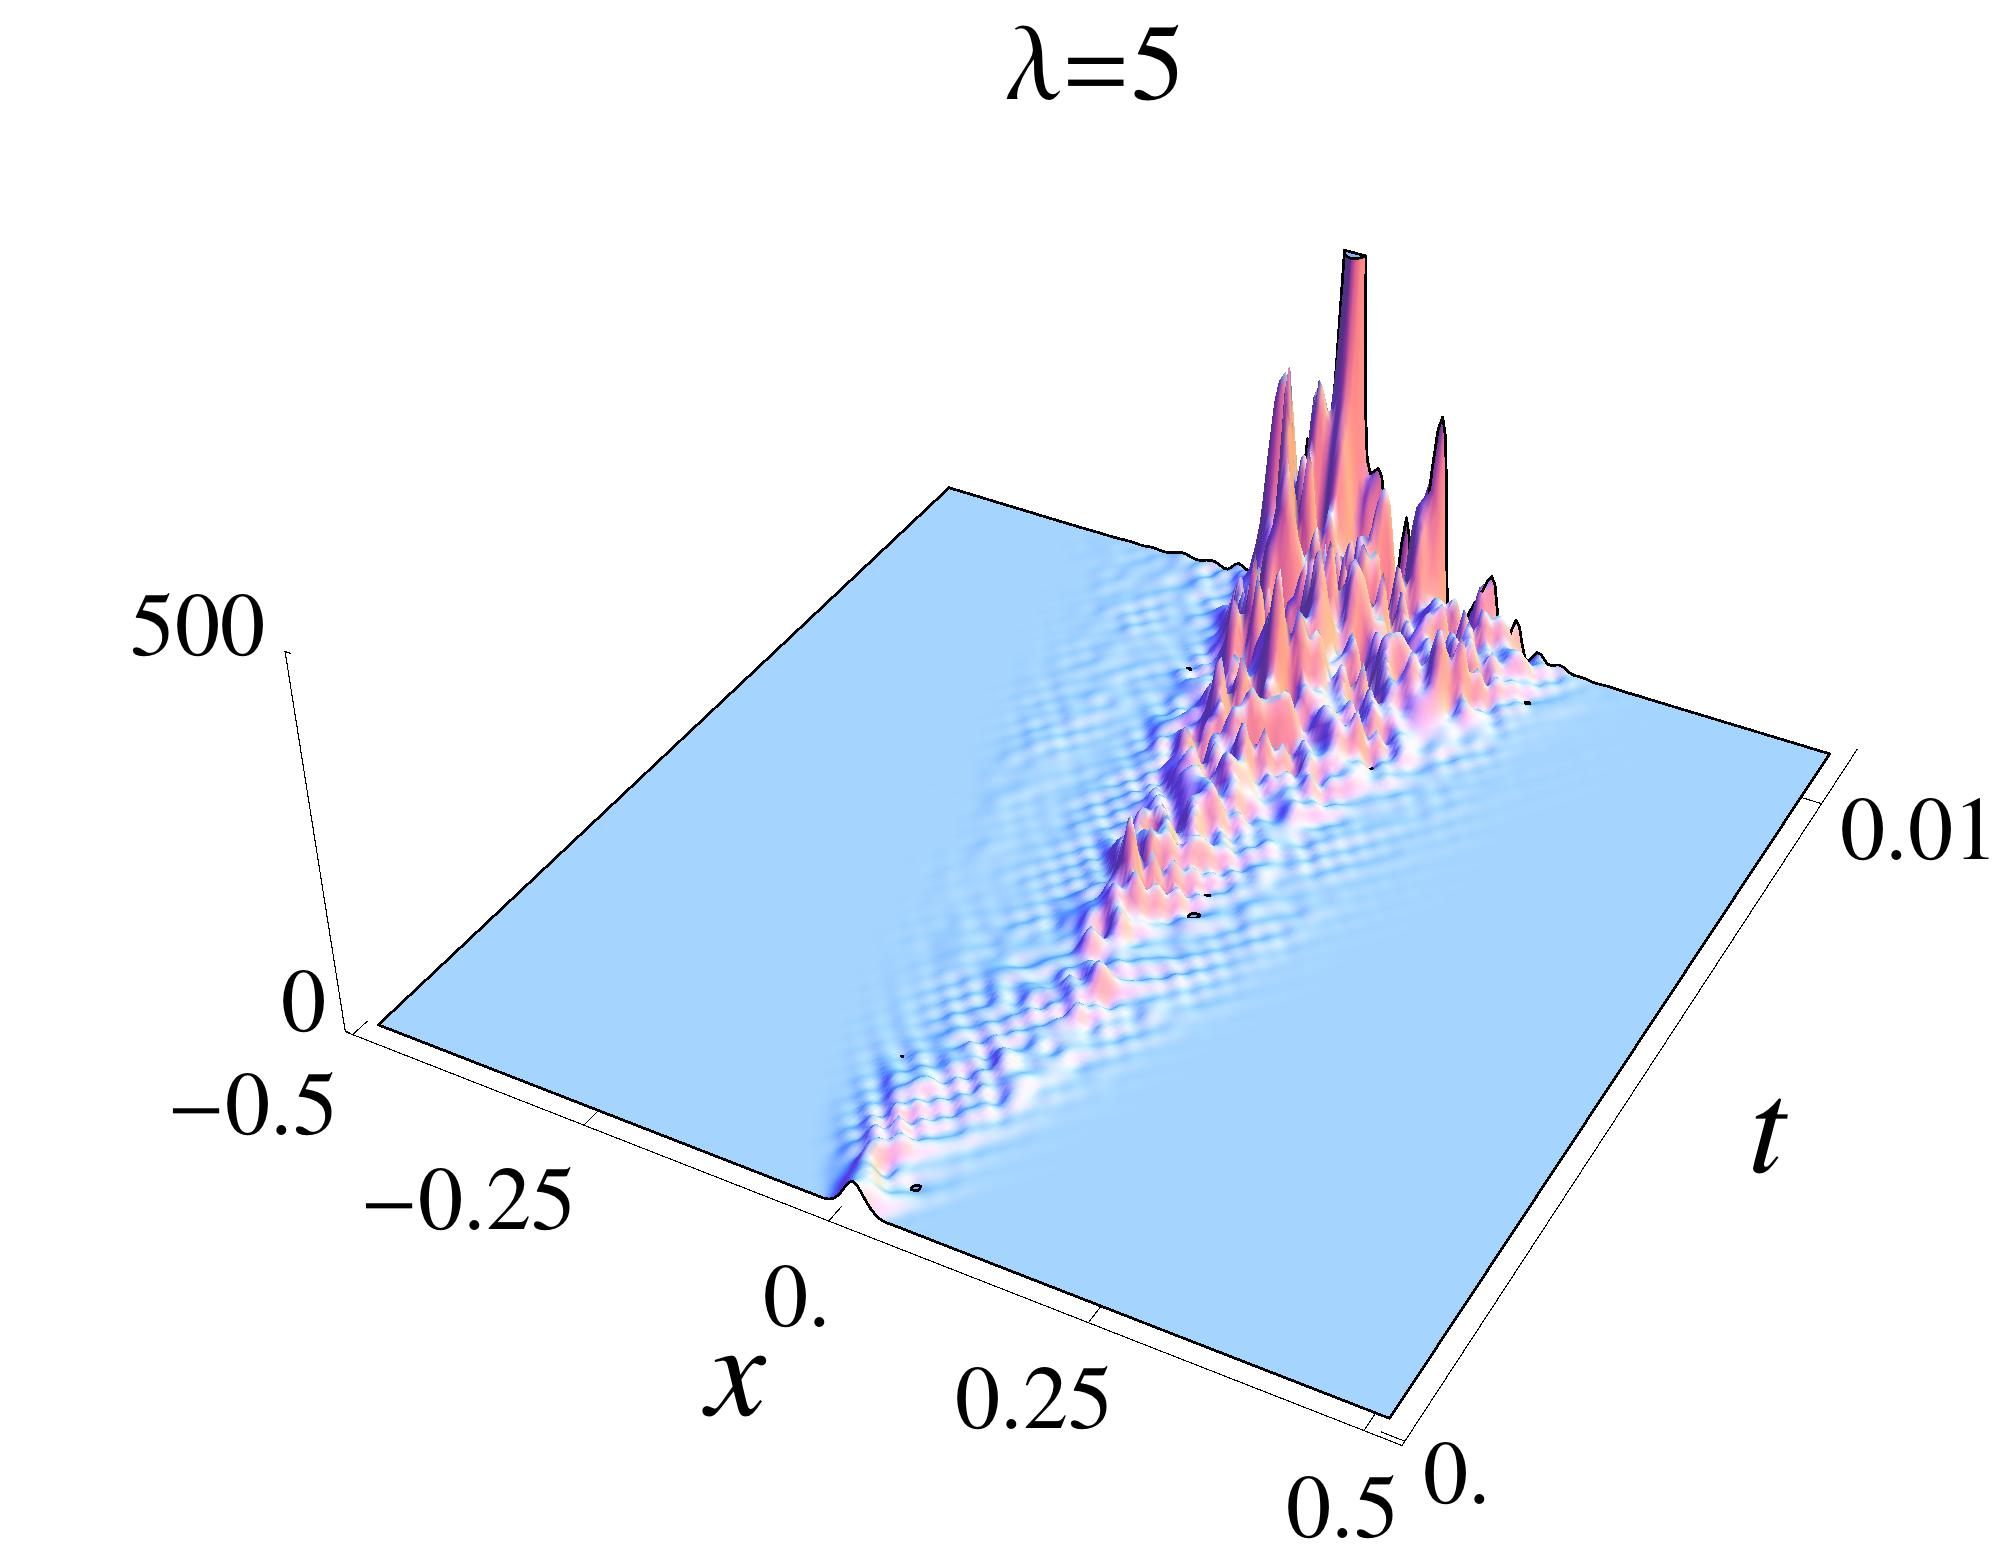
\includegraphics[scale=0.05]{figs/small_Delta_L5_cut.jpeg}
    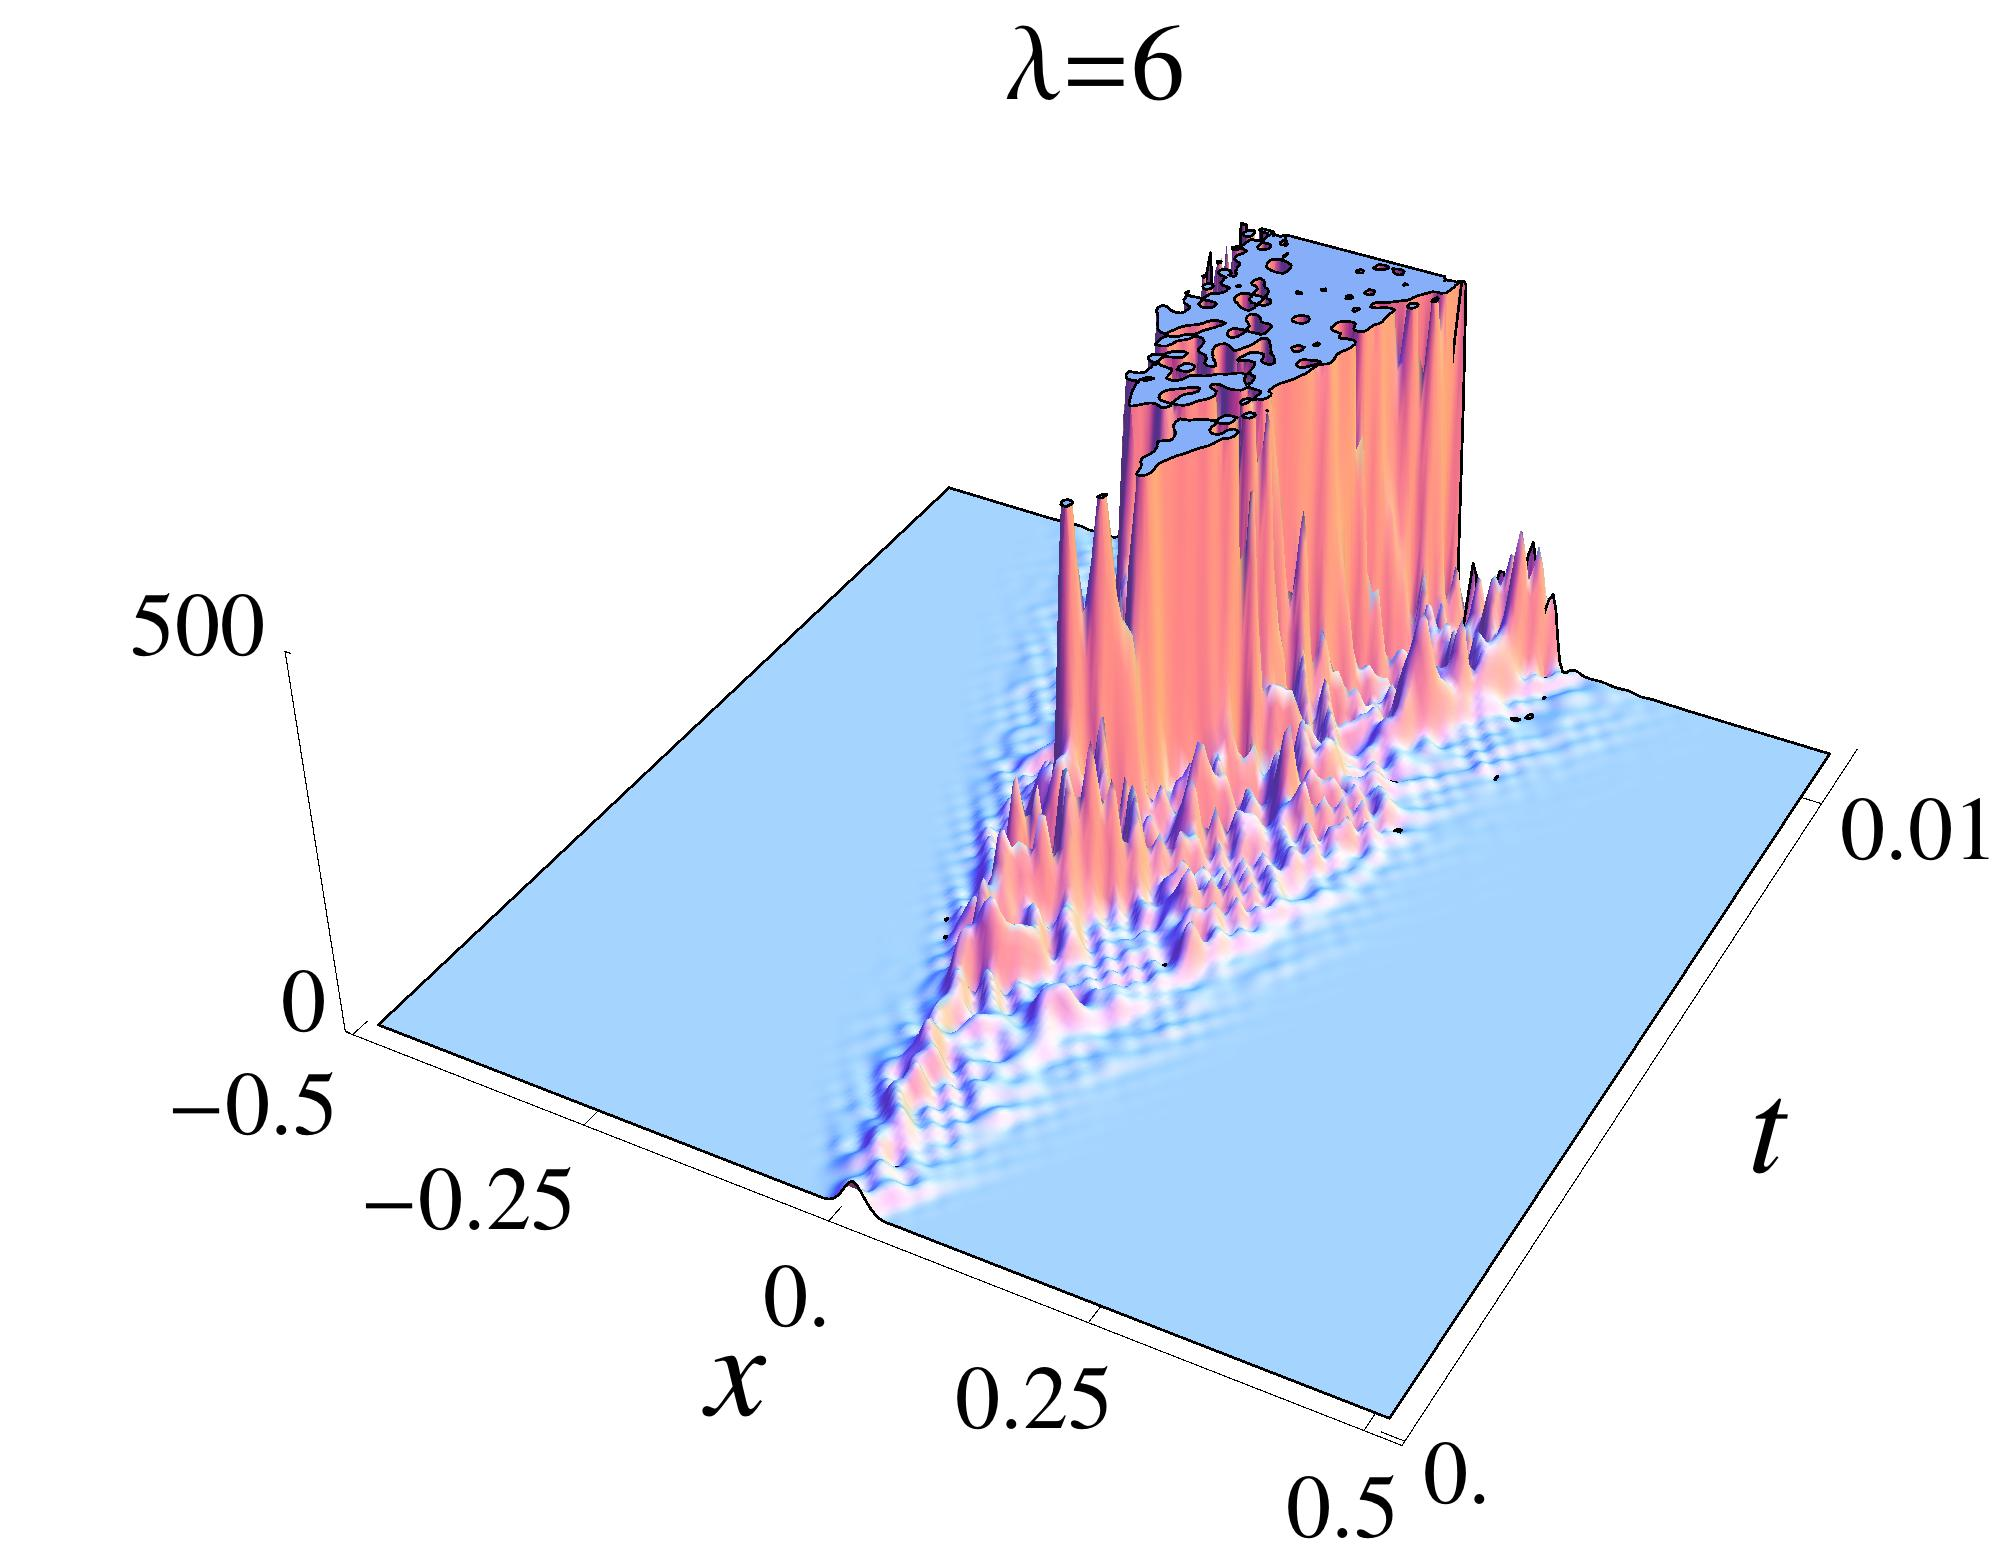
\includegraphics[scale=0.05]{figs/small_Delta_L6_cut.jpeg}
    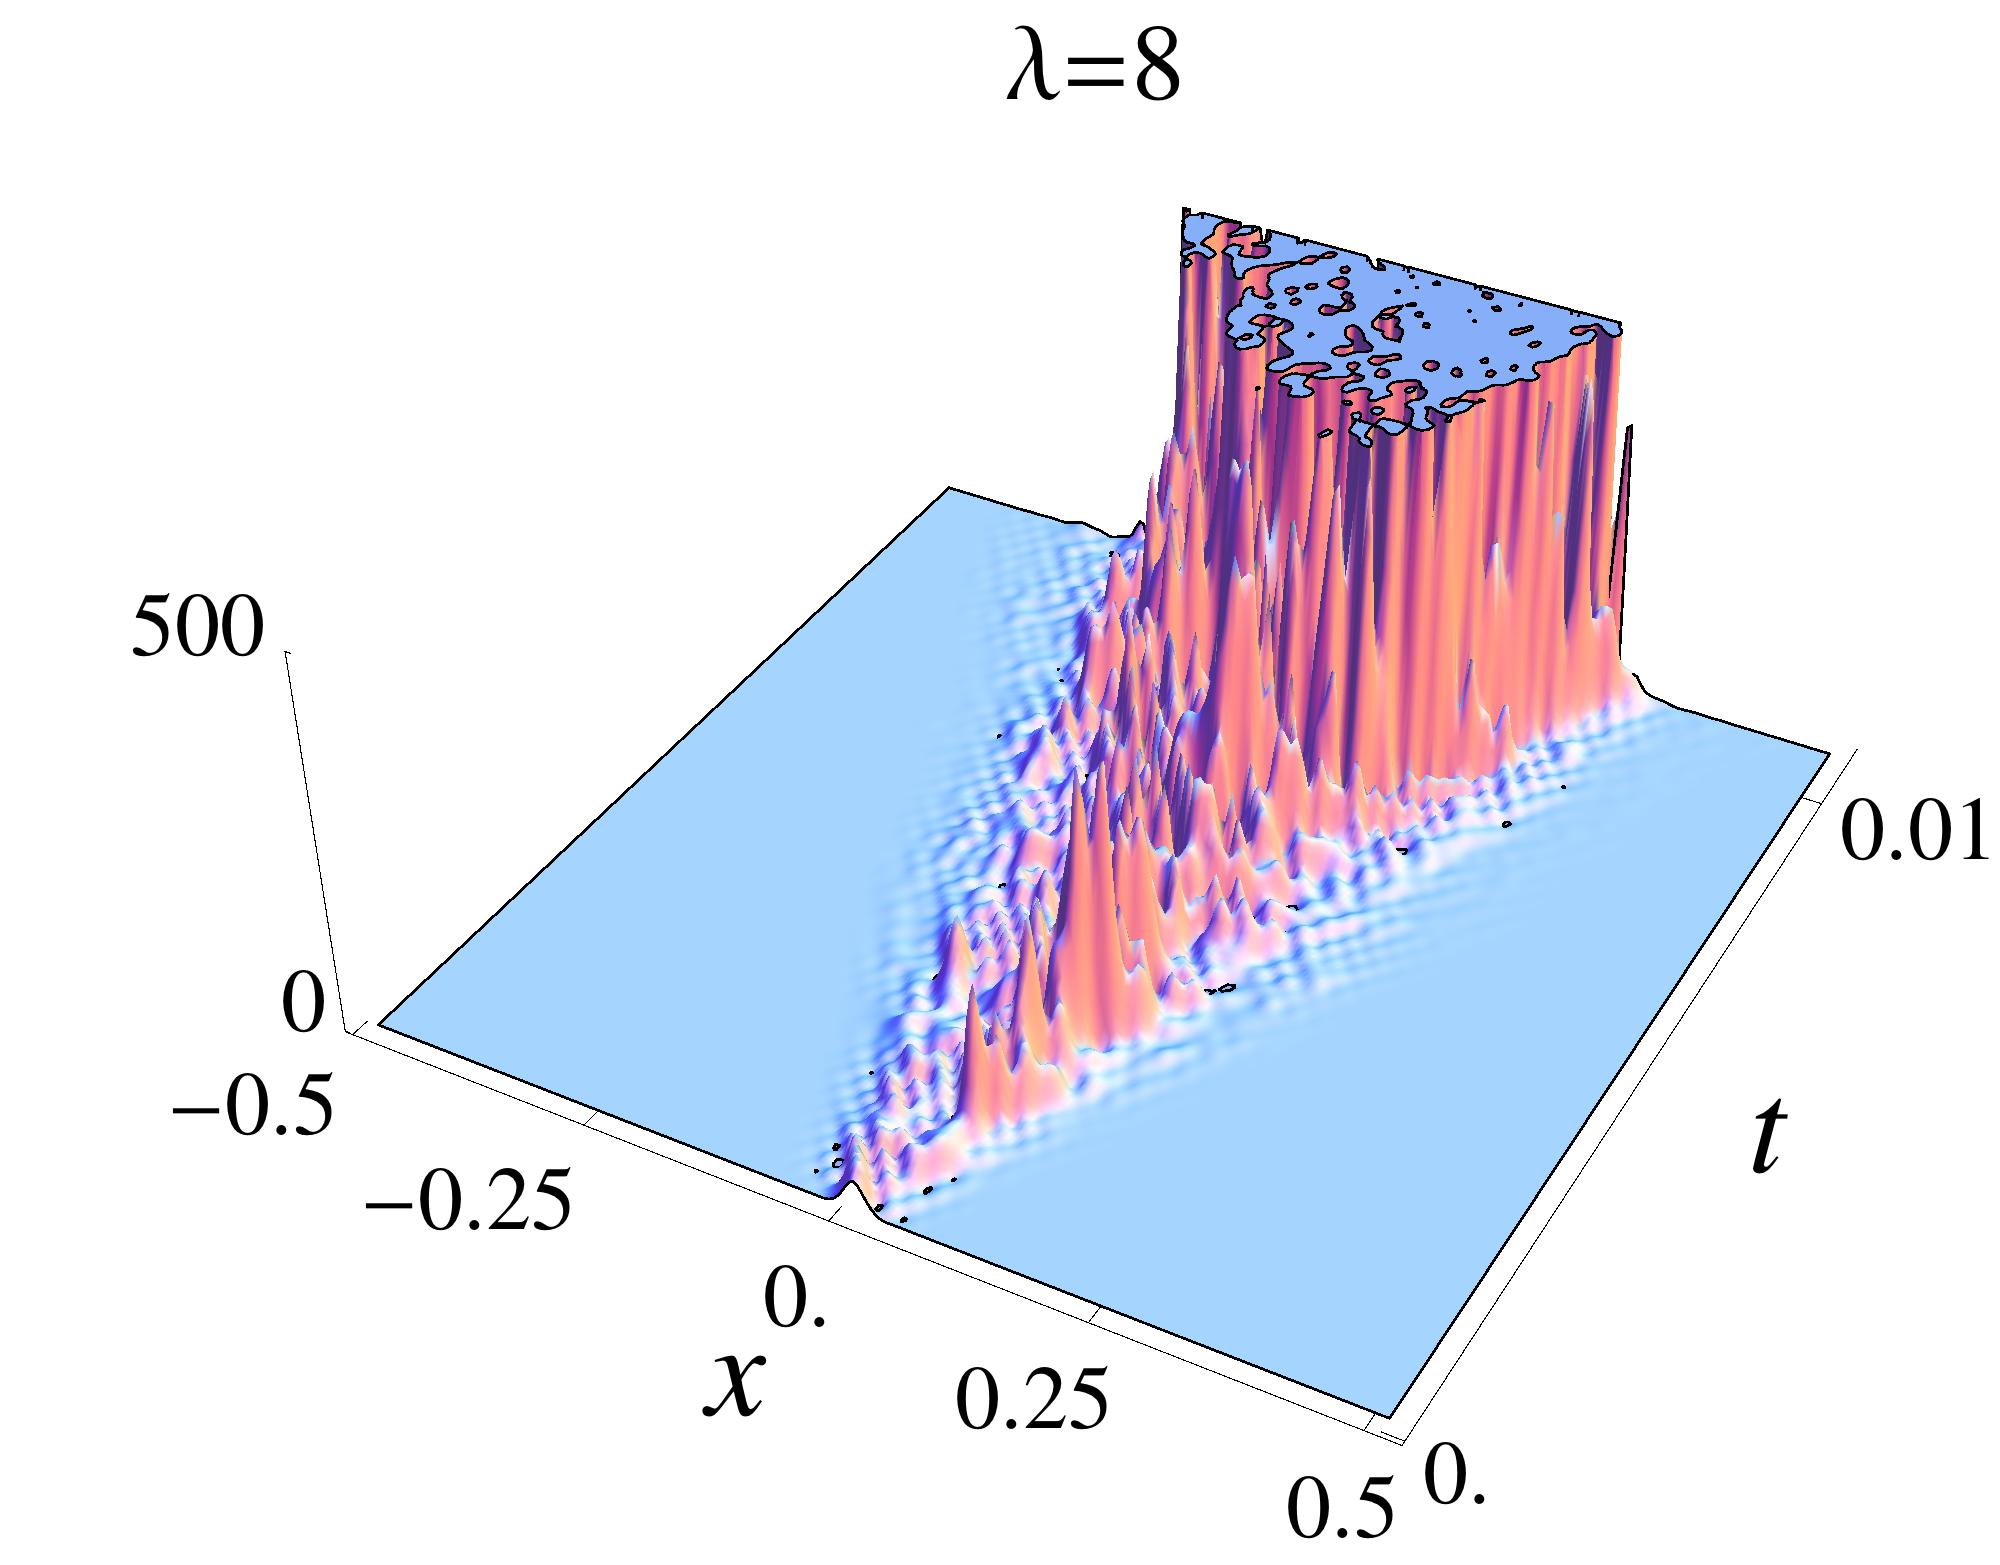
\includegraphics[scale=0.05]{figs/small_Delta_L8_cut.jpeg}
    \only<8>{\phantom{aaa}\\[3.3em]
    \phantom{aaaaaa}}
    }
\end{frame}
\section{Fractional PDE -- the tool to bridge the two worlds}
\begin{frame} % Fundamental Solution.
  \begin{align*}
    \textcolor{contrast_color_2}{G_H(t,x)} \pause = (2\pi t)^{-d/2} \exp\left(-\frac{\Norm{x}^2}{2t}\right)\quad t>0, x\in\R^d
  \end{align*}
  \bigskip \pause
  \begin{center}
    ------ v.s. ------
  \end{center}
  \bigskip
  \begin{align*}
  \hspace{-2em}
    \textcolor{contrast_color_1}{G_W(t,x)} = \pause
    \begin{cases}
      \displaystyle \frac{1}{2}1_{\{|x|<t\}}                                                                                                                  & \text{if $d=1$}         \\[1em]
      \displaystyle \frac{1}{2\pi} \frac{1}{\sqrt{t^2-|x|^2}}1_{\{|x|<t\}}                                                                                    & \text{if $d=2$}         \\[1em]
      \displaystyle \frac{1}{4\pi t}\sigma_t                                                                                                                  & \text{if $d=3$}         \\[2em]
      \displaystyle C_d\left[ \left(t^{-1}\partial_t\right)^{\frac{d-3}{2}}\left(t^{d-2}\int_{|y|=1}\delta_0(x+ty)\ud\sigma(y)\right)\right]                  & \text{if $d\ge 3$ odd}  \\[2em]
      \displaystyle C_d'\left[ \left(t^{-1}\partial_t\right)^{\frac{d-2}{2}}\left(t^{d-1}\int_{|y|=1}\frac{\delta_0(x+ty)}{\sqrt{1-|y|^2}}\ud y\right)\right] & \text{if $d\ge 2$ even} \\[1em]
    \end{cases}
  \end{align*}
\end{frame}
\begin{frame} % Fourier transform of Heat and Wave Kernel
    \begin{center}
      \begin{tikzpicture}[scale=1, transform shape]
        \tikzset{>=latex}
        \draw[->, contrast_color_2] (-1,0) -- (3, 0) node [right] {Re};
        \draw[->, contrast_color_1] (0,-1) -- (0,3) node [above] {Im};
        \filldraw [black] (0,0) circle (0.04);
        \draw [gray] (0,0) circle (0.04);
        \pause
        \node[contrast_color_2] (HE) at (1.7,0.2) {Heat};
        \node[rotate=90,contrast_color_1] (WE) at (-0.2,1.7) {Wave};
        % \draw[->,dashed] (e) -- (HE);
        % \draw[->,dashed] (e) -- (WE);
        \pause
        \node[] () at (2,4) {$\textcolor{contrast_color_1}{\mathcal{F} G_W(t,\cdot) (\xi) = \dfrac{\sin(t|\xi|)}{|\xi|}=\text{Im} \dfrac{\e^{it|\xi|}}{|\xi|}}$};
        \node[] () at (2.5,-0.5) {$\textcolor{contrast_color_2}{\mathcal{F} G_H(t,\cdot) (\xi) = \e^{- t |\xi|^2}}$};
        \pause
        \node[] () at (8,4) {$\textcolor{contrast_color_1}{\mathcal{L}\mathcal{F} G_W(\circ,\cdot) (s,\xi) = \dfrac{1}{s^2+|\xi|^2}}$};
        \node[] () at (8,-0.5) {$\textcolor{contrast_color_2}{\mathcal{L}\mathcal{F} G_H(\circ,\cdot) (s,\xi) = \dfrac{1}{s+|\xi|^2}}$};
        \pause
        \node[] () at (2,2) {\Huge \textcolor{contrast_color_3}{?}};
        \node[] () at (8,2) {\Huge \textcolor{contrast_color_3}{?}};
      \end{tikzpicture}
    \end{center}
\end{frame}
\begin{frame}[fragile] % Fourier and Laplace transforms
  \begin{gather*}
    \hspace{-1.2em}
    \left(\partial^b_t + (-\Delta)^{a/2}\right)\: u(t,x) = I^r_t f(t,x), \quad
    u(t,x) = \int_0^t \int_{\R^d} \textcolor{contrast_color_3}{G_{a,b,r,d}(t-s,x-y)} f(s,y) \ud s \ud y
  \end{gather*}
  \mySeparateLine
  \pause
  \begin{center}
    \begin{tikzpicture}[scale=1, transform shape]
      \tikzset{>=latex}
      \draw[->, contrast_color_2] (-0.6,0) -- (3, 0) node [right] {Re};
      \draw[->, contrast_color_1] (0,-0.6) -- (0,3) node [above] {Im};
      \filldraw [black] (0,0) circle (0.04);
      \draw [gray] (0,0) circle (0.04);
      \node[contrast_color_2] (HE) at (1.7,0.2) {Heat};
      \node[rotate=90,contrast_color_1] (WE) at (-0.2,1.7) {Wave};
      % \draw[->,dashed] (e) -- (HE);
      % \draw[->,dashed] (e) -- (WE);
      \node[] () at (2,4) {$\textcolor{contrast_color_1}{\mathcal{F} G_W(t,\cdot) (\xi) = \dfrac{\sin(t|\xi|)}{|\xi|}=\text{Im} \dfrac{\e^{it|\xi|}}{|\xi|}}$};
      \node[] () at (2.5,-0.5) {$\textcolor{contrast_color_2}{\mathcal{F} G_H(t,\cdot) (\xi) = \e^{- t |\xi|^2}}$};
      \node[] () at (8.5,4) {$\textcolor{contrast_color_1}{\mathcal{L}\mathcal{F} G_W(\circ,\cdot) (s,\xi) = \dfrac{1}{s^2+|\xi|^2}}$};
      \node[] () at (8.5,-0.5) {$\textcolor{contrast_color_2}{\mathcal{L}\mathcal{F} G_H(\circ,\cdot) (s,\xi) = \dfrac{1}{s+|\xi|^2}}$};
      \pause
      \node[] () at (2.5,1.8) {$\textcolor{contrast_color_3}{t^{\Ceil{b}+r-1}E_{b,b+r}\left(-t^b |\xi|^a\right)}$};
      \pause
      \node[] () at (8.6,1.8) {$\textcolor{contrast_color_3}{\dfrac{s^{-r}}{s^b+|\xi|^a}}$};
    \end{tikzpicture}
  \end{center}
\end{frame}
\begin{frame}[fragile] % Expression of G

  \begin{align*}
    \mathcal{L}\mathcal{F} \textcolor{contrast_color_3}{G_{a,b,r,d}(\circ,\cdot)} (s,\xi) = \frac{s^{-r}}{s^b+|\xi|^a}
  \end{align*}

  \begin{align*}
    \Downarrow
  \end{align*}

  \begin{align*}
    \mathcal{F} \textcolor{contrast_color_3}{G_{a,b,r,d}(t,\cdot)} (\xi) = t^{\Ceil{b}+r-1} E_{b,b+r}\left(-t^b |\xi|^a\right)
  \end{align*}

  \begin{align*}
    \Downarrow
  \end{align*}

  \begin{align*}
    \textcolor{contrast_color_3}{G_{a,b,r,d}(t,x)}
       = \pi^{-d/2} |x|^{-d}t^{b+r-1}
       \FoxH{2,1}{2,3}{\frac{ |x|^a}{2^{a-1}\nu t^b}}
       {(1,1),\:(b+r,b)}{(d/2,a/2),\:(1,1),\:(1,a/2)}
  \end{align*}
\end{frame}
\begin{frame}[fragile,t] % Fundamental solutions -- Y(1,x)
  \begin{center}
    $\textcolor{contrast_color_3}{G_{2,\beta,0,1}(1,x)}$ with \footnote{\textcolor{refcolor}{C. Hu and Nualart}, SPA, 2019.}
    % $\beta=15/8$, $5/3$, $3/2$, $1$, $3/4$, $1/2$, and $1/8$
    \vfill

    \begin{tikzpicture}[scale=1, transform shape]
      \tikzset{>=latex}
      \node[] (b) at (0,0) {$\beta \quad = \quad (\textcolor{contrast_color_1}{2},) \quad 15/8, \quad 5/3, \quad  3/2,\quad \textcolor{contrast_color_2}{1}, \quad  3/4, \quad 1/2, \quad 1/8$};
      \node[] (w) at (-2.7,-1.3) {\textcolor{contrast_color_1}{$\dfrac{1}{2}1_{[-1,1]}(x)$}};
      \draw [->,contrast_color_1] (w) --++ (0,1);
      \node[] (h) at (1.2,-1.3) {\textcolor{contrast_color_2}{$\dfrac{1}{\sqrt{2\pi}}e^{-\frac{x^2}{2}}$}};
      \draw [->,contrast_color_2] (h) --++ (0,1);
    \end{tikzpicture}
    \bigskip

    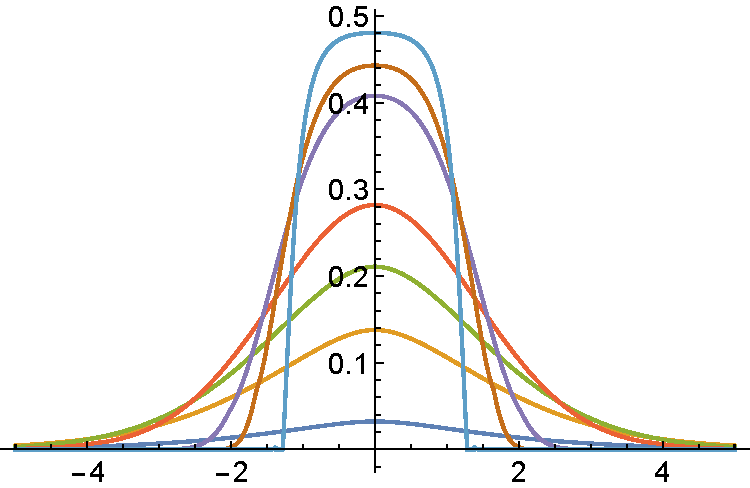
\includegraphics[scale=0.5]{./figs/TimeFrac-Green-Y.pdf}
  \end{center}
\end{frame}
\begin{frame}[fragile,t] % Fundamental solutions -- Y(t,x)
 \begin{center}
    $\textcolor{contrast_color_3}{G_{2,\beta,0,1}(t,x)}$ with \footnote{\textcolor{refcolor}{C. Hu and Nualart}, SPA, 2019.}
    \vfill

    \begin{tikzpicture}[scale=1, transform shape]
      \tikzset{>=latex}
      \node[] (b) at (0,0) {$\beta \quad = \quad (\textcolor{contrast_color_1}{2},) \qquad 15/8, \qquad  3/2, \qquad  6/5, \qquad (\textcolor{contrast_color_2}{1})$};
      \node[] (w) at (-2,-1.3) {\textcolor{contrast_color_1}{$\dfrac{1}{2}1_{[-t,t]}(x)$}};
      \draw [->,contrast_color_1] (w) --++ (0,1);
      \node[] (h) at (3.26,-1.3) {\textcolor{contrast_color_2}{$\dfrac{1}{\sqrt{2\pi t}}e^{-\frac{x^2}{2t}}$}};
      \draw [->,contrast_color_2] (h) --++ (0,1);
    \end{tikzpicture}
    \vfill

    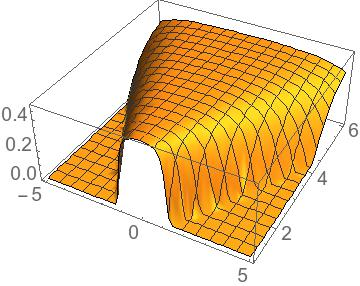
\includegraphics[scale=0.25]{figs/TimeFrac-GreenYST15-8.jpeg} \quad
    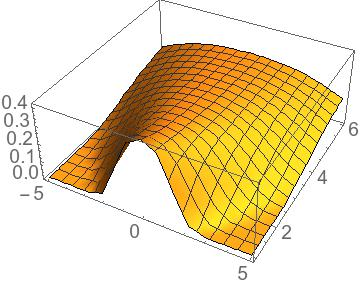
\includegraphics[scale=0.25]{figs/TimeFrac-GreenYST3-2.jpeg}  \quad
    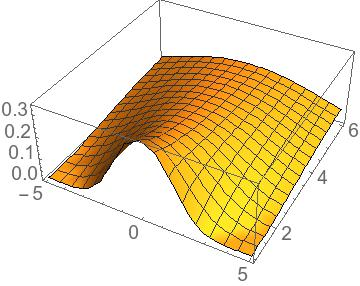
\includegraphics[scale=0.25]{figs/TimeFrac-GreenYST6-5.jpeg}
    \vfill

    \footnotesize $(t,x)\in [1,6]\times [-5,5]$
 \end{center}
\end{frame}
\begin{frame}[fragile,t] % Tail
 \begin{center}

   {\small
   \begin{align*}
     A_a = -\pi^{-d/2}\nu 2^{ a -1}\frac{\Gamma((d+ a )/2)}{\Gamma(2 b +r)\Gamma(- a /2)}
   \end{align*}}

   \vfill
   \mySeparateLine
   \vfill

   \begin{align*}
     \textcolor{contrast_color_3}{G_{ a , b ,r,d}(1,x)} \sim
      \begin{cases}
         \quad A_{ a } \: |x|^{-(d+ a )}                           & \text{if $ a \ne 2$}         \\[1.6em]
         % \makebox[\linewidth]{\rule{0.3\paperwidth}{0.4pt}}        \\[2em]
         \rule{0.3\paperwidth}{0.4pt}                              & \rule{0.1\paperwidth}{0.4pt} \\[2em]
         \quad A_{2}   \: |x|^{\alpha}\exp\left(-\beta|x|^c\right) & \text{if $ a =2$}
      \end{cases} \qquad  \text{as $|x|\to\infty$}
   \end{align*}

   \bigskip
   \mySeparateLine

   \small
   \begin{align*}
     A_{ 2 }= \pi^{-d/2} (2- b )^{d/2-( b +r)} b ^{\frac{ b (d+2-2( b +r))}{2(2- b )}}(2\nu)^{\frac{2( b +r)-(d+2)}{2(2- b )}}
   \end{align*}
   \begin{align*}
     \alpha = \frac{d( b -1)-2( b +r-1)}{2- b }, \quad
     \beta  = (2- b ) b ^{\frac{ b }{2- b }}(2\nu)^{\frac{1}{ b -2}}, \qquad
     c      = \frac{2}{2- b }.
   \end{align*}
 \end{center}
\end{frame}
\begin{frame}[fragile] % Nonnegativity of fundamental solutions
  \centering
  When is $\textcolor{contrast_color_3}{G_{a,b,r,d}(t,x)}$ nonnegative?
  \bigskip \pause

  \begin{tikzpicture}[scale=2.2]
    \draw [->] (-0.3,0) -- (2.3,0) node [right] {$a$};
    \draw [->] (0,-0.3) -- (0,2.2) node [above] {$b$};
    \draw [densely dashed,gray] (1,0) -- (1,2) (2,0) -- (2,2) (0,1) -- (2.5,1) (0,2) -- (2,2);
    \draw (1,0.05) -- (1,-0.05) node [below] {$1$};
    \draw (2,0.05) -- (2,-0.05) node [below] {$2$};
    \draw (0.05,1) -- (-0.05,1) node [left] {$1$};
    \draw (0.05,2) -- (-0.05,2) node [left] {$2$};
    \filldraw [fill=contrast_color_2, opacity=0.5] (0,0) rectangle (2,1);
    \filldraw [fill=contrast_color_1, opacity=0.5] (1,1) -- (2,1) -- (2,2);
    \draw [thick] (1.03,1.03) -- (1.97,1.97);
    \draw [thick] ([shift=(0:0.05)]1,1) arc (0:90:0.05);
    \draw [thick] ([shift=(180:0.05)]2,2) arc (180:270:0.05);
    \node at (2.3,1.5) [rotate=90, anchor=center] {$1\le d\le 3$};
    \node at (2.3,0.45)[rotate=90, anchor=center] {$d\ge 1$};
    \draw [thick] (0.03,1) -- (2,1);
    \draw [thick] ([shift=(-90:0.05)]0,1) arc (-90:90:0.05);
    \node at (1.73,1.35) [rotate=45, anchor=center] {$r\ge 0$};
    \node at (1,0.45) {$r\ge 0$};
    % \node at (1,0.9) {$r=0$ or $r>1$};
    \node at (1.5,1.55) [rotate=45,anchor=south] {$r>\frac{d+3}{2}-b$};
  \end{tikzpicture}

  \begin{center}
    \small \textcolor{refcolor}{C., Hu, Nualart, 19}
  \end{center}

\end{frame}
\section{One case study of SPDEs in two worlds}
\begin{frame} % Noise -- Introduce mu and gamma
    \begin{align*}
      \E[W(\varphi) W(\psi)] =  \int_{\mathbb{R}^d} \cF \varphi(\xi) \overline{\cF \psi(\xi)}\textcolor{contrast_color_2}{\mu(d\xi)} = (2\pi)^d \iint_{\R^{2d}} \varphi(x) \psi(y) \textcolor{contrast_color_1}{\gamma(x-y)} dxdy
    \end{align*}

    \begin{minipage}{0.2\textwidth}\phantom{a} \end{minipage}\hfill
    \begin{minipage}{0.78\textwidth}
    \begin{center}
    \begin{tabular}{ccc}
     \textcolor{contrast_color_2}{\it spectral measure} &                       & \textcolor{contrast_color_1}{\it correlation function} \\ [4em]
     nonnegative                                        & $\Longleftrightarrow$ & nonnegative definite                                   \\ [1em]
     nonnegative definite                               & $\Longleftrightarrow$ & nonnegative                                            \\
    \end{tabular}
    \end{center}
    \end{minipage}
    \vfill
    \pause

    \begin{minipage}{0.2\textwidth}\phantom{a} \end{minipage}\hfill
    \begin{minipage}{0.78\textwidth}
    \begin{center}
    \renewcommand{\arraystretch}{1.2}
      \begin{tabular}{|c|c|c|c|c|}
 \cline{1-2} \cline{4-5}
 \textcolor{contrast_color_2}{$\mu=\varphi(\xi)$} & \textcolor{contrast_color_1}{$\gamma(x)$} &  & \multicolumn{2}{c|}{\textcolor{assumption_color}{Assumptions}}         \\ \cline{1-2} \cline{4-5}
        $C_{d,\alpha}|\xi|^{-(d-\alpha)}$                & $|x|^{-\alpha}$                           &  & \multicolumn{2}{c|}{\textcolor{assumption_color}{A}: $\alpha\in(0,d)$} \\ \cline{1-2} \cline{4-5}
 $(2\pi)^{-d}$                                    & $\delta_0$                                &  & \textcolor{assumption_color}{B}: $d=1,2$                                & \textcolor{assumption_color}{C}: $d=3$ \\ \cline{1-2} \cline{4-5}
      \end{tabular}
    \end{center}
    \end{minipage}
    % \begin{minipage}{0.3\textwidth} \textcolor{contrast_color_2}{\it spectral measure}\end{minipage} \hfill
    % \begin{minipage}{0.3\textwidth} \textcolor{contrast_color_1}{\it correlation function}\end{minipage}
    % \begin{minipage}{0.2\textwidth}\phantom{a} \end{minipage}\hfill
    % \begin{minipage}{0.78\textwidth}
    %   \begin{center}
    %     nonnegative $\Longrightarrow$ nonnegative definite
    %   \end{center}
    % \end{minipage}\hfill
\end{frame}
\begin{frame} % Problem itself
\begin{equation*}
  % \tag{SWE}
 \left\{\begin{array}{rcl}
  \displaystyle \frac{\partial^2 u}{\partial t^2}(t,x) & = & \Delta u(t,x) + \sqrt{\theta}\,u(t,x)\dot{W}(x), \quad t>0,\: x \in \mathbb{R}^d \\[2ex]
  \displaystyle u(0,x) & = & 1, \qquad \displaystyle \frac{\partial u}{\partial t}(0,x)  =  0
 \end{array}\right.
  \end{equation*}
  \vfill
  \begin{itemize}
    \item Time-independent centered Gaussian noise:
    \begin{align*}
      \E[W(\varphi) W(\psi)] =  \int_{\mathbb{R}^d} \cF \varphi(\xi) \overline{\cF \psi(\xi)}\mu(d\xi) =: \langle \varphi,\psi \rangle_{\cH}
    \end{align*}
    \end{itemize}
    \mySeparateLine
    \bigskip
    \begin{center}
    \begin{minipage}{0.6\textwidth}
    \centering
    \pause
    Question:
    \bigskip

    \begin{itemize}
      \item Well-posedness
      \item Exact large-time/moment asymptotics
    \end{itemize}
    \end{minipage}
    \end{center}
\end{frame}
\begin{frame}[fragile,t] % Skorohod solution
  \begin{center}
    Mild solution (in Skorohod sense)
  \end{center}
  \begin{equation*}
    u(t,x) = 1 + \sqrt{\theta}\int_0^t \left( \int_{\R^d} G(t-s,x-y)u(s,y) W(\delta y) \right)\ud s
  \end{equation*}
  \bigskip

  \pause
  Solved through
  \begin{align*}
    u(t,x) = 1 + \sum_{n=1}^\infty \theta^{n/2}I_n(f_n(\cdot,x,t))
  \end{align*}
  where
  \begin{align*}
    f_n(x_1,...,x_k;x,t) = \int_0^t \int_0^{t_n}\cdots \int_0^{t_2} G(t-t_n,x-x_n)\cdots G(t_2-t_1,x_2-x_1) \ud t_1\cdots \ud t_n
  \end{align*}
\end{frame}
\begin{frame}[fragile,t] % Mild solution
  \begin{center}
    Mild solution (in Skorohod sense)
  \end{center}
  \begin{equation*}
    u(t,x) = 1 + \sqrt{\theta}\int_0^t \left( \int_{\R^d} G(t-s,x-y)u(s,y) W(\delta y) \right)\ud s
  \end{equation*}
  \bigskip


  It is well known that\footnote{$\widetilde{f_n}(x_1,...,x_k; x, t) = \frac{1}{n!} \sum_{\rho \in \Sigma_n} f_n\left(x_{\rho(1)},\cdots, x_{\rho(n)}\right)$}

  \begin{gather*}
   \text{$L^2(\Omega)$ solution exists on $\left(0,T\right)\times\R^d$} \\[1em]
    \huge\Updownarrow                                                   \\[1em]
    \mathbb{E}\left(u(t,x)^2\right) = \sum_{n \ge 0} \theta^n n!  \Norm{\widetilde{f_n}(\cdot,x,t)}_{\mathcal{H}^{\otimes n}}^2<\infty \quad \forall (t,x) \in (0,T) \times \R^d
  \end{gather*}

\end{frame}
\begin{frame}[fragile,t] % Norm scaling
 \begin{center}
   How to get sharp estimate of $\Norm{\widetilde{f_n}(\cdot,x,t)}_{\mathcal{H}^{\otimes n}}^2$?
 \end{center}
 \pause
 \mySeparateLine
 \bigskip

 By scaling property:
 \begin{align*}
 \Norm{ \widetilde{f_n}\left(\cdot,0,t\right) }_{ \mathcal{H}^{\otimes n} }^2
    & = \Norm{ \widetilde{f_n}(\cdot,0,1) }_{ \mathcal{H}^{\otimes n} }^2  t^{ \textcolor{gray!80!black}{\left[ 2(b+r)-\frac{b \alpha}{a} \right]} n}
 \end{align*}
 so we only need to show how fast the following function decays in $n$:
 \begin{align*}
   n \mapsto \Norm{ \widetilde{f_n}\left(\cdot,0,1\right) }_{ \mathcal{H}^{\otimes n} }^2
 \end{align*}
\end{frame}
\begin{frame}[fragile,t] % Laplace probing
  \begin{center}
    How to get sharp estimate of $\Norm{\widetilde{f_n}(\cdot,x,t)}_{\mathcal{H}^{\otimes n}}^2$?
  \end{center}
  \pause
  \mySeparateLine
  \bigskip
  \begin{center}
    We want to use Laplace transform to probe the growth in $t$ in terms of $n$:
    \begin{align*}
      n \mapsto \textcolor{contrast_color_1}{\int_0^\infty \e^{-t} \Norm{ \widetilde{f}_n(\cdot,0,t) }_{\mathcal{H}^{\otimes n}}^2 \ud t}
    \end{align*}
  \end{center}
  \pause
  \bigskip
  \begin{itemize}
    \item[E.g.] $\int_0^\infty \e^{-t} \textcolor{cyan!50!black}{t^{n}}\ud t = 1/(\Gamma\left(n+1\right))$ for all $n>-1$.
      \bigskip
    \item[] $\int_0^\infty \e^{-t}\textcolor{cyan!50!black}{\e^{\sqrt{t} }}\ud t = \dfrac{1}{2} \sqrt[4]{\e} \sqrt{\pi } \left(\Erf\left(1/2\right)+1\right)+1\approx 2.730$.
      \bigskip
    \item[] $\int_0^\infty \e^{-t}\textcolor{cyan!50!black}{\e^{-\sqrt{t} }}\ud t =1-\dfrac{1}{2} \sqrt[4]{\e} \sqrt{\pi}\: \Erfc\left(1/2\right)\approx 0.454$.
      \bigskip
    \item[] $\int_0^\infty \e^{-t}\textcolor{cyan!50!black}{\sin(t)}\ud t =\int_0^\infty \e^{-t}\textcolor{cyan!50!black}{\cos(t)}\ud t = 1/2$.
      \bigskip
    \item[] $\int_0^\infty \e^{-t}\textcolor{cyan!50!black}{1}\ud t = 1$.
  \end{itemize}
\end{frame}
\begin{frame}[fragile] % Diagonalization

  \textit{Diagonalization:} \quad \pause Let $\gamma = K*K$ and define
  \begin{align*}
    H_n(t, \vec{x}) & = n! \int_{(\R^d)^n} \prod_{k=1}^n K(x_k - y_k) \widetilde{f_n}(\vec{y};0,t) \ud \vec{y}
  \end{align*}
  so that
  \begin{align*}
    \Norm{\widetilde{f_n}(\cdot,0;t)}_{\mathcal{H}^{\otimes n}}^2 = \frac{1}{(n!)^2}\int_{(\R^d)^n} H_n^2(t,\vec{x}) \ud \vec{x}
  \end{align*}
\end{frame}
\begin{frame}[fragile,t] % Computations
  \begin{align*}
         & \textcolor{contrast_color_1}{\int_0^\infty \e^{-t} \Norm{ \widetilde{f}_n(\cdot,0,t) }_{\mathcal{H}^{\otimes n}}^2 \ud t}                            \\ \pause
     =   & \int_0^\infty \e^{-t} \frac{1}{(n!)^2}\int_{\R^{nd}} H_n^2(t,\vec{x}) \ud \vec{x} \ud t                                                              \\ \pause
     =   & \textcolor{grayout}{\frac{2^{n(2(b+r) - b\alpha/a)}}{(n!)^2}} \int_0^\infty 2e^{-2t} \int_{\R^{nd}} H_n(t,\vec{x})^2 \ud \vec{x} \ud t              \\ \pause
     \le & \textcolor{grayout}{\frac{2^{n(2(b+r) - b\alpha/a)}}{(n!)^2}} \int_{\R^{nd}} \left[ \int_0^\infty \e^{-t} H_n(t,\vec{x}) \ud t\right ]^2 \ud \vec{x} \\ \pause
     =   & \textcolor{grayout}{\frac{2^{n(2(b+r) - b\alpha/a)}}{(n!)^2}} \int_{\R^{nd}} \left[\sum_{\sigma \in \Sigma_n} \prod_{k=1}^n \textcolor{contrast_color_3}{\frac{1}{1+\frac{\nu}{2}\left|\sum_{j=k}^n \xi_{\sigma(j)} \right|^a}}\right]^2 \mu(\ud \vec{\xi})
 \end{align*}
  \pause
  where
  \begin{align*}
    \textcolor{contrast_color_3}{\frac{1}{1+\frac{\nu}{2}\left|\xi\right|^a}} = \mathcal{L}\mathcal{F} G\left(1,\xi\right).
  \end{align*}
  \pause
  Recall that
  \begin{align*}
    \textcolor{contrast_color_2}{\mathcal{L}\mathcal{F} G_H (s,\xi) = \frac{1}{s+|\xi|^2}}
    \quad \text{and} \quad
    \textcolor{contrast_color_1}{\mathcal{L}\mathcal{F} G_W (s,\xi) = \frac{1}{s^2+|\xi|^2}}
  \end{align*}
\end{frame}
\begin{frame}[fragile,t] % Decorrelation
  \begin{align*}
         & \textcolor{contrast_color_1}{\int_0^\infty \e^{-t} \Norm{ \widetilde{f}_n(\cdot,0,t) }_{\mathcal{H}^{\otimes n}}^2 \ud t} \\ \pause
     \le & \textcolor{grayout}{\frac{2^{n(2(b+r) - b\alpha/a)}}{(n!)^2}} \underbrace{\int_{(\R^d)^n} \left[\sum_{\sigma \in \Sigma_n} \prod_{k=1}^n
     \textcolor{contrast_color_3}{\frac{1}{1+\frac{\nu}{2}\left|\sum_{j=k}^n \xi_{\sigma(j)} \right|^a}}\right]^2 \mu(\ud \vec{\xi})}_{\text{\large $:=T_n$}}
 \end{align*}
  \pause
  \mySeparateLine
  \bigskip

  Decorrelation shows that $T_n \le C^n$. \pause Hence,
\end{frame}
\begin{frame}[fragile,t] % Computations -- Done
  \begin{align*}
 \Norm{ \widetilde{f_n}\left(\cdot,0,t\right) }_{ \mathcal{H}^{\otimes n} }^2
  & =  t^{ \left[ 2(b+r)-\frac{b \alpha}{a} \right] n} \Norm{ \widetilde{f_n}(\cdot,0,1) }_{ \mathcal{H}^{\otimes n} }^2                                                                                                                                            \\ \pause
  & =  t^{ \left[ 2(b+r)-\frac{b \alpha}{a} \right] n} \frac{1}{ \Gamma\left( \left[ 2(b+r)- \frac{b \alpha}{a} \right] n +1 \right) }  \textcolor{contrast_color_1}{\int_0^\infty \e^{-t} \Norm{ \widetilde{f_n}(\cdot,0,t) }_{ \mathcal{H}^{\otimes n} }^2 \ud t} \\ \pause
  & \le  t^{ \left[ 2(b+r)-\frac{b \alpha}{a} \right] n} \frac{1}{ \Gamma\left( \left[ 2(b+r)- \frac{b \alpha}{a} \right] n +1 \right) } \frac{2^{n(2(b+r) - b\alpha/a)}}{(n!)^2} T_n                                                                               \\ \pause
  & \le  t^{ \left[ 2(b+r)-\frac{b \alpha}{a} \right] n} \frac{1}{ \Gamma\left( \left[ 2(b+r)- \frac{b \alpha}{a} \right] n +1 \right) } \frac{2^{n(2(b+r) - b\alpha/a)}}{(n!)^2} C^n                                                                               \\ \pause
  & \asymp t^{[2(b + r ) -b \alpha / a]n} \dfrac{ \left(2^{ \left[ 2(b+r)- \frac{b \alpha}{a} \right]}C\right)^n }{ (n!)^{ 2(b+r) + 2 - b\alpha/a }}
  \end{align*}

  \bigskip
  \pause
  Therefore,
 \begin{align}
  \nonumber
  \Norm{u(t,x)}_2^2 & \le \sum_{n \ge 0} \theta^n t^{[2(b + r ) -b \alpha / a]n} \dfrac{ \left(2^{ \left[ 2(b+r)- \frac{b \alpha}{a} \right]}C' \right)^n }{ (n!)^{ 2(b+r) + 1 - b\alpha/a }},
  \label{E:2nomBd}
 \end{align}
 which is finite provided that
 \begin{equation*}
  2(b+r) + 1 - \frac{b\alpha}{a} > 0.
 \end{equation*}
\end{frame}
\begin{frame}[fragile,t] % Can we make it even sharper?
 \begin{center}
    Can we make it even sharper?
 \end{center}
 \mySeparateLine
 \pause
 Indeed, with slightly more effort, one can show that the \textit{reverse Cauchy-Schwatz inequality} above is not too bad:
\begin{align*}
  \lim_{n \to \infty}  \frac{1}{n} \log\left(\textcolor{contrast_color_1}{\int_0^\infty \e^{-t} \Norm{ \widetilde{f}_n(\cdot,0,t) }_{\mathcal{H}^{\otimes n}}^2 \ud t}\right) = \log\left(\textcolor{grayout}{2^{2(b+r)-\frac{b\alpha}{a} }}\rho_{\nu,a}(\gamma)\right)
\end{align*}
where
\begin{gather*}
 \rho_{\nu,a}(\gamma) = \sup_{\Norm{f}_{L^2(\R^d)} =1} \int_{\R^d} \left[ \int_{\R^d} \frac{f(x+y)f(y)}{\sqrt{1+\frac{\nu}{2}|x+y|^a } \sqrt{1+\frac{\nu}{2}|y|^a} } \ud y \right]^2 \mu(\ud x)
\end{gather*}
\bigskip

and \textcolor{refcolor}{Bass, X. Chen and Rosen 09} showed that
\bigskip

\begin{align*}
  \rho_{\nu,a}(\gamma) = \nu^{-\alpha/a} \mathcal{M}_a^{2-(\alpha / a)}(\gamma)
\end{align*}

\bigskip
\pause
Therefore, we can find the exact convergence radius -- or $T_{2}$ -- for $\Norm{u(t,x)}_2^2$.
\end{frame}
\begin{frame}<2->[fragile] % Variational const. M
\begin{align*}
  \mathcal{M}_{a,d}(\gamma,\theta) & := \sup_{g \in \mathcal{F}_a} \left\{ \left\langle g^2 * g^2, \gamma \right\rangle_{L^2(\R^d)}^{1/2} - \frac{\theta}{2}\: \mathcal{E}_a(g,g) \right\}
\end{align*}
\begin{center}
\bigskip

\begin{minipage}{0.75 \textwidth}
\begin{itemize}
  \item $\displaystyle \mathcal{E}_a(g,g) := (2\pi)^{-d} \int_{\R^d} |\xi|^a |\mathcal{F}g(\xi)|^2 \ud \xi$
    \bigskip
  \item $ \displaystyle \mathcal{F}_a := \left\{f\in L^2(\R^d): \: \Norm{f}_{L^2(\R^d)}=1,\: \mathcal{E}_a(f,f)<\infty \right\}$
\end{itemize}
\end{minipage}
\end{center}
\end{frame}
\begin{frame}[fragile,t] %  Smoothing vs Roughening -- call back

\begin{align*}
  \mathcal{M}_{a,d}(\gamma,\theta) & := \sup_{g \in \mathcal{F}_a} \left\{ \left\langle g^2 * g^2, \textcolor{contrast_color_1}{\gamma} \right\rangle_{L^2(\R^d)}^{1/2} - \frac{\theta}{2}\: \textcolor{contrast_color_2}{\mathcal{E}_a}(g,g) \right\}
\end{align*}

\bigskip
\begin{center}
  \begin{tabular}{ c c c  }
    $\textcolor{contrast_color_2}{-(-\Delta)^{a/2} u}$ &  & \textcolor{contrast_color_1}{$\dot{W} u$} \\ [0.5em] \hline \\
    Smoothing  &  & Roughening  \\
  \end{tabular}
  \bigskip

  \begin{tikzpicture}
    \path (0,0) rectangle (0.35\paperwidth,0.4\paperheight);
    \node[scope fading=north,inner sep=0pt,outer sep=0pt,anchor=center] at(0.2\paperwidth,0.2\paperheight) {
\includegraphics[height=0.4\paperheight]{figs/picture-tug-war2.jpg}};
  \end{tikzpicture}
\end{center}
\end{frame}
\begin{frame}[fragile,t] %  Upgrading from second moment to $p$-th moment...
 \begin{center}
    Upgrading from second moment to $p$-th moment...
 \end{center}
 \pause
 \bigskip

 \begin{enumerate}
   \item Upper bound:  hypercontractivity
     \begin{align*}
      \Norm{u(t,x)}_p \le \Norm{u_{(p-1)\theta}(t,x)}_2,  \qquad \text{for all $p\ge 2$, $t>0$ and $x\in\R^d.$}
     \end{align*}
     \bigskip
   \item Lower bound: Construct/find the exact function that achieves the upper bound.
 \end{enumerate}
\end{frame}
\begin{frame}[fragile,t] % More SPDEs?
 \begin{center}
   More general SPDEs?
 \end{center}
\bigskip

We have seen that all we need \underline{seem to} be
  \begin{align}
    \tag{$\star$}
    \mathcal{L}\mathcal{F} G\left(1,\xi\right) = \textcolor{contrast_color_3}{\frac{1}{1+\frac{\nu}{2}\left|\xi\right|^a}}
  \end{align}
  with
  \begin{align*}
    \textcolor{contrast_color_2}{\mathcal{L}\mathcal{F} G_H (s,\xi) = \frac{1}{s+|\xi|^2}}
    \quad \text{and} \quad
    \textcolor{contrast_color_1}{\mathcal{L}\mathcal{F} G_W (s,\xi) = \frac{1}{s^2+|\xi|^2}}
  \end{align*}
  \pause
  \mySeparateLine
  \bigskip

  \begin{center}
    Indeed, we do have a class of SPDEs,   \\
    the fundamental solutions $G$ of which \\
    do satisfy $(\star)$:
  \end{center}
\end{frame}
\begin{frame}[fragile] % Yes, more SPDEs
  \centering

In \textcolor{refcolor}{C., Hu, Nualart 19}, we have studied:
\vfill

\begin{equation*}
  \begin{cases}
    \left(\partial^b_t + \frac{\nu}{2}(-\Delta)^{a/2}\right)\: u(t,x) = I^r_t \left[\sqrt{\theta}\: u(t,x)\: \dot W(x) \right] & \text{$x\in \R^d$, $t>0$}, \\
    u(0,\cdot) = 1                                                                                                             & b \in (0,1],               \\
    u(0,\cdot) = 1, \quad \partial_t u(0,\cdot) = 0                                                                            & b \in (1,2),
  \end{cases}
\end{equation*}
\vfill

 for $a \in (0,2]$, $b \in (0,2)$, $r\ge 0$, $\nu > 0$ and $\theta>0$.

% \bigskip
% \bigskip
% \pause
%
% \begin{align*}
%     \mathcal{L}\mathcal{F} G\left(s,\xi\right) = \textcolor{contrast_color_3}{\frac{s^{-r}}{s^{b}+\frac{\nu}{2}\left|\xi\right|^a}}
% \end{align*}
% \bigskip \pause

\end{frame}
\begin{frame}[fragile] % Fourier and Laplace transforms
  \begin{align*}
    \left(\partial^b_t + (-\Delta)^{a/2}\right)\: u(t,x) = I^r_t \left[\sqrt{\theta}\: u(t,x)\: \dot W(x) \right]
  \end{align*}
  \pause
  \begin{center}
    \begin{tikzpicture}[scale=1, transform shape]
      \tikzset{>=latex}
      \draw[->, contrast_color_2] (-0.6,0) -- (3, 0) node [right] {Re};
      \draw[->, contrast_color_1] (0,-0.6) -- (0,3) node [above] {Im};
      \filldraw [black] (0,0) circle (0.04);
      \draw [gray] (0,0) circle (0.04);
      \node[contrast_color_2] (HE) at (1.7,0.2) {Heat};
      \node[rotate=90,contrast_color_1] (WE) at (-0.2,1.7) {Wave};
      % \draw[->,dashed] (e) -- (HE);
      % \draw[->,dashed] (e) -- (WE);
      \node[] () at (2,4) {$\textcolor{contrast_color_1}{\mathcal{F} G_W(t,\cdot) (\xi) = \dfrac{\sin(t|\xi|)}{|\xi|}=\text{Im} \dfrac{\e^{it|\xi|}}{|\xi|}}$};
      \node[] () at (2.5,-0.5) {$\textcolor{contrast_color_2}{\mathcal{F} G_H(t,\cdot) (\xi) = \e^{- t |\xi|^2}}$};
      \node[] () at (8.5,3) {$\textcolor{contrast_color_1}{\mathcal{L}\mathcal{F} G_W(\circ,\cdot) (s,\xi) = \dfrac{1}{s^2+|\xi|^2}}$};
      \node[] () at (8.5,+0.5) {$\textcolor{contrast_color_2}{\mathcal{L}\mathcal{F} G_H(\circ,\cdot) (s,\xi) = \dfrac{1}{s+|\xi|^2}}$};
      \pause
      \node[] () at (2.5,1.8) {$\textcolor{contrast_color_3}{t^{\Ceil{b}+r-1}E_{b,b+r}\left(-2^{-1}\nu t^b |\xi|^a\right)}$};
      \pause
      \node[] () at (8.6,1.8) {$\textcolor{contrast_color_3}{\dfrac{s^{-r}}{s^b+|\xi|^a}}$};
    \end{tikzpicture}
  \end{center}
  \vfill \pause \bigskip

  \begin{center}
    In particular, by taking $s=1$, we have $\mathcal{L}\mathcal{F} G\left(1,\xi\right) = \textcolor{contrast_color_3}{\dfrac{1}{1+\left|\xi\right|^a}}$
  \end{center}

\end{frame}
\begin{frame}[fragile,t] % Interpolated PDE figures -- Fourier and Laplace transforms.
  \begin{center}
  Exact solvability \footnote{\textcolor{refcolor}{Balan, L. Chen \& X. Chen,} AIHP 2021.}
  \bigskip

  \begin{tikzpicture}[scale=0.6]
     % \draw [thick,dashed] (2,0) -- (2,5.5);
    \node[contrast_color_2] (a) at (2.5,6) {SHE};
    \draw [->] (-0.3,0) -- (5.5,0) node [right] {$\alpha$};
    \draw [->] (0,-0.3) -- (0,5.5) node [above] {$d$};
    \foreach \x in {1,...,5}{
      \draw (\x,0.1)--++(0,-0.2) node [below] {$\x$};
      \draw (0.1,\x)--++(-0.2,0) node [left] {$\x$};
      \draw (\x,\x) + (-0.15,-0.15) rectangle +(0.15,0.15);
      \draw [thick] ([shift=(-90:0.1)]0,\x) arc (-90:90:0.1);
      \draw [thin, dotted] (\x,0) -- (\x, 5.4);
    }
    \filldraw[contrast_color_2] (0, 1) + (0.1, -0.05) rectangle +(1,0.05);%\filldraw (1,1) circle (0.05);
    \filldraw[contrast_color_2] (0, 2) + (0.1, -0.05) rectangle +(1.9,0.05);
    \filldraw[contrast_color_2] (0, 3) + (0.1, -0.05) rectangle +(1.9,0.05);
    \filldraw[contrast_color_2] (0, 4) + (0.1, -0.05) rectangle +(1.9,0.05);
    \filldraw[contrast_color_2] (0, 5) + (0.1, -0.05) rectangle +(1.9,0.05);
    \filldraw[contrast_color_2,very thick] (1, 1) + (0, -0.14)  -- +(0,0.14);
    \draw[contrast_color_2!60!white] (2,2) circle (0.11);
    \draw[contrast_color_2!60!white] (2,3) circle (0.11);
    \draw[contrast_color_2!60!white] (2,4) circle (0.11);
    \draw[contrast_color_2!60!white] (2,5) circle (0.11);
    \draw[contrast_color_2!30!white] (2, 3) + (0.1, -0.05) rectangle +(1,0.05);
    \draw[contrast_color_2!30!white] (2, 4) + (0.1, -0.05) rectangle +(2,0.05);
    \draw[contrast_color_2!30!white] (2, 5) + (0.1, -0.05) rectangle +(3,0.05);
  \end{tikzpicture}
  \hspace{5em}
  \begin{tikzpicture}[scale=0.6]
    % \draw [thick,dashed] (3,0) -- (3,5.5);
    \node[contrast_color_1] (a) at (2.5,6) {SWE};
    \draw [->] (-0.3,0) -- (5.5,0) node [right] {$\alpha$};
    \draw [->] (0,-0.3) -- (0,5.5) node [above] {$d$};
    \foreach \x in {1,...,5}{
     \draw (\x,0.1)--++(0,-0.2) node [below] {$\x$};
     \draw (0.1,\x)--++(-0.2,0) node [left] {$\x$};
     \draw (\x,\x) + (-0.15,-0.15) rectangle +(0.15,0.15);
     \draw [thick] ([shift=(-90:0.1)]0,\x) arc (-90:90:0.1);
     \draw [thin, dotted] (\x,0) -- (\x, 5.4);
    }
    \filldraw[contrast_color_1] (0, 1) + (0.1, -0.05) rectangle +(1,0.05);%\filldraw (1,1) circle (0.05);
    \filldraw[contrast_color_1] (0, 2) + (0.1, -0.05) rectangle +(2,0.05);%\filldraw (2,2) circle (0.05);
    \filldraw[contrast_color_1] (0, 3) + (0.1, -0.05) rectangle +(2.9,0.05);%\filldraw (3,3) circle (0.05);
    % \filldraw (0, 4) + (0.1, -0.05) rectangle +(2.9,0.05);
    % \filldraw (0, 5) + (0.1, -0.05) rectangle +(2.9,0.05);
    % \draw (2,2) circle (0.11);
    \draw[contrast_color_1!60!white] (3,3) circle (0.11);
    % \draw (3,4) circle (0.11);
    % \draw (3,5) circle (0.11);
    % \draw (2, 3) + (0.1, -0.05) rectangle +(1,0.05);
    % \draw (2, 4) + (0.1, -0.05) rectangle +(2,0.05);
    \draw[contrast_color_1!30!white, dashed] (0, 5) + (0.1, -0.05) rectangle +(5,0.05);
    \draw[contrast_color_1!30!white, dashed] (0, 4) + (0.1, -0.05) rectangle +(4,0.05);
    \filldraw[contrast_color_1,very thick] (1, 1) + (0, -0.14)  -- +(0,0.14);
    \filldraw[contrast_color_1,very thick] (2, 2) + (0, -0.14)  -- +(0,0.14);
  \end{tikzpicture}

  \vfill
  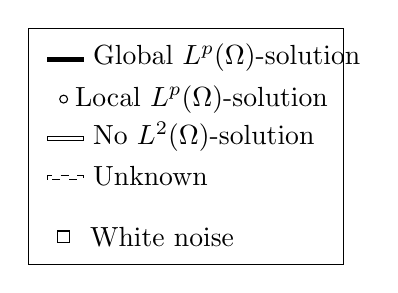
\begin{tikzpicture}[scale=0.5]
    \def\x{5}
    \draw (-0.4,-4.2+\x) rectangle +(8,6);
    \filldraw (0, 1+\x) + (0.1, -0.05) rectangle +(1,0.05) node [right] {Global $L^p(\Omega)$-solution};
    \draw (0.5,0+\x) circle (0.1); \node at (4,0+\x) {Local $L^p(\Omega)$-solution};
    \draw (0, -1+\x) + (0.1, -0.05) rectangle +(1,0.05) node [right] {No $L^2(\Omega)$-solution};
    \draw[dashed] (0, -2+\x) + (0.1, -0.05) rectangle +(1,0.05) node [right] {Unknown};
    \draw (0.5, 1.5) + (-0.15,-0.15) rectangle +(0.15,0.15); \node at (3,1.5) {White noise};
    % \draw[white] (0,-1.5) circle (0.01);
  \end{tikzpicture}
  \end{center}
\end{frame}
\begin{frame}[fragile] % A figure for the nested T
  \begin{center}
    Exact phase transition in case of local solution
  \end{center}
  \vfill

  \begin{tikzpicture}[baseline]
    % \draw[help lines] (0,0) grid (8,5);
    \draw [very thick, ->] (0,0) -- (10,0) node [right] {$t$};
    \draw (1,-0.3) -- (1,0.3) node [above] {$0$};
    \draw (7,-0.3) -- (7,0.3) node [above] {$T_2$};
    \draw (6,-0.3) -- (6,0.3) node [above] {$T_3$};
    \draw (4,-0.3) -- (4,0.3) node [above] {$T_p$};
    \draw (5,0.3) -- (5,0.3) node [above] {$\cdots$};
    \draw [postaction={decorate,
    decoration={text along path,
          text={|\color{contrast_color_2}|{$L^2(\Omega)$} solution exists}, raise=-7pt,
          text align={center},
    },
       },
       ] (1,0) .. controls (2,-3) .. (7,0);
    \draw [postaction={decorate,
    decoration={text along path,
          text={|\color{contrast_color_2}|{$L^3(\Omega)$} solution exists}, raise=-7pt,
          text align={center},
    },
       },
       ] (1,0) .. controls (2,-2) .. (6,0);
    \draw [postaction={decorate,
    decoration={text along path,
          text={|\color{contrast_color_2}|{$L^p(\Omega)$} solution exists}, raise=-7pt,
          text align={center},
    },
       },
       ] (1,0) .. controls (2,-0.5) .. (4,0);
    \draw [dashed, thick, postaction={decorate,
    decoration={text along path,
          text={|\color{contrast_color_1}|{No $L^2(\Omega)$} solutions}, raise=3pt,
          text align={center},
    },
       },
       ] (7,0) .. controls (7.8,1.2) .. (10,1.5);
  \end{tikzpicture}
\end{frame}
\begin{frame}[fragile] % Theorem -- Exact asymptotics
  \begin{theorem}[Exact Asymptotics \textcolor{refcolor}{\small [Balan-C.-Chen 21]}]
    \begin{enumerate}[(i)]
    \item Under \textcolor{assumption_color}{Assumption A} with $0<\alpha<d\le 3$, by setting
     \begin{align*}
      t_p := (p-1)^{1/(4-\alpha)}t,
     \end{align*}
     it holds that
     \begin{align*}
      \lim_{t_p\to \infty}t_p^{-\frac{4-\alpha}{3-\alpha}}\log \Norm{u(t,x)}_p
      &= \theta^{\frac{1}{3-\alpha}}
	     \left(\frac{1}{2}\right)^{\frac{\alpha}{2(3-\alpha)}}
	 \frac{3-\alpha}{2}
	 \left(\frac{2\cM^{1/2}}{4-\alpha}\right)^{\frac{4-\alpha}{3-\alpha}}.
     \end{align*}
     % In particular, by freezing an arbitrary $p\ge 2$ and $t>0$, we have that
     % \begin{equation*}
     %  % \label{E:tMain}
	%   \hspace{-2em}
     %  \lim_{t\to \infty} t^{-\frac{4-\alpha}{3-\alpha}} \log \E \left(|u(t,x)|^p\right)
     %  =p (p-1)^{\frac{1}{3-\alpha}} \theta^{\frac{1}{3-\alpha}}
     %  \left(\frac{1}{2} \right)^{\frac{\alpha}{2(3-\alpha)}} \frac{3-\alpha}{2}
     %  \left( \frac{2\cM^{1/2}}{4-\alpha}\right)^{\frac{4-\alpha}{3-\alpha}}
     % \end{equation*}
	% and respectively,
     % \begin{equation*}
     %  % \label{E:pMain}
	%   \hspace{-2em}
     %  \lim_{p\to \infty} p^{-\frac{4-\alpha}{3-\alpha}} \log \E\left(|u(t,x)|^p\right)
     %  = t^{\frac{4-\alpha}{3-\alpha}}\theta^{\frac{1}{3-\alpha}}
     %  \left(\frac{1}{2} \right)^{\frac{\alpha}{2(3-\alpha)}}\frac{3-\alpha}{2}
     %  \left( \frac{2\cM^{1/2}}{4-\alpha}\right)^{\frac{4-\alpha}{3-\alpha}}.
     % \end{equation*}
	\vspace{1em}
    \item Under \textcolor{assumption_color}{Assumption B}, results in (i) are still true provided that all $\alpha$'s and $\cM$'s in part (i) are replaced by $d$ and $\cM(\delta_0)$, respectively.
    \end{enumerate}
 \end{theorem}
\end{frame}
\begin{frame}[fragile] % Plot the contour lines or equipotential lines
\begin{center}
 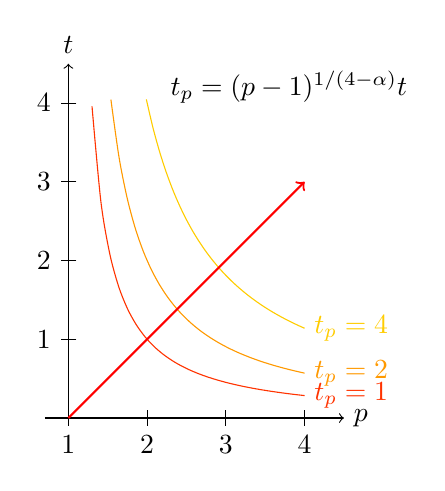
\begin{tikzpicture}[scale=1]
  % \draw[scale=0.5, domain=-3:3, smooth, variable=\x, blue] plot ({\x}, {\x*\x});
  % \draw[scale=0.5, domain=-3:3, smooth, variable=\y, red]  plot ({\y*\y}, {\y});
  \begin{scope}
    \draw[->] (0.7, 0) -- (4.5, 0) node[right] {$p$};
    \draw[->] (1, -0.1) -- (1, 4.5) node[above] {$t$};
    % The following is for alpha=1/2.
    \draw[scale=1, domain=1.30:4, smooth, variable=\p, red!80!yellow]  plot ({\p}, {(\p-1)^(-8/7)*1}) node [right] {$t_p=1$};
    \draw[scale=1, domain=1.54:4, smooth, variable=\p, red!40!yellow]  plot ({\p}, {(\p-1)^(-8/7)*2}) node [right] {$t_p=2$};
    \draw[scale=1, domain=1.99:4, smooth, variable=\p, red!20!yellow]  plot ({\p}, {(\p-1)^(-8/7)*4}) node [right] {$t_p=4$};
  \end{scope}
  \foreach \p in {1,...,4}{
      \draw (\p,0.1)--++(0,-0.2) node [below] {$\p$};
  }
  \foreach \t in {1,...,4}{
      \draw (1.1, \t)--++(-0.2,0) node [left] {$\t$};
  }
  \draw [thick, ->, red] (1,0) -- (4,3);
  \node at (3.8,4.2) {$t_p=(p-1)^{1/(4-\alpha)}t$};
\end{tikzpicture}
\end{center}
\vfill
\begin{gather*}
  \lim_{t_p\to \infty}\big[\underbrace{\textcolor{contrast_color_1}{(p-1)^{1/(4-\alpha)}t}}_{=t_p}\big]^{-\frac{4-\alpha}{3-\alpha}}\log \Norm{u(t,x)}_p
  \\ || \\
 \theta^{\frac{1}{3-\alpha}}
         \left(\frac{1}{2}\right)^{\frac{\alpha}{2(3-\alpha)}}
     \frac{3-\alpha}{2}
     \left(\frac{2\cM^{1/2}}{4-\alpha}\right)^{\frac{4-\alpha}{3-\alpha}}
\end{gather*}
\end{frame}
\begin{frame}[fragile] % Plot: Two special directions.
  \begin{align*}
    \lim_{t_p\to \infty}\big[\underbrace{\textcolor{contrast_color_1}{(p-1)^{1/(4-\alpha)}t}}_{=t_p}\big]^{-\frac{4-\alpha}{3-\alpha}}\log \Norm{u(t,x)}_p
    = \theta^{\frac{1}{3-\alpha}}
    \left(\frac{1}{2}\right)^{\frac{\alpha}{2(3-\alpha)}}
    \frac{3-\alpha}{2}
    \left(\frac{2\cM^{1/2}}{4-\alpha}\right)^{\frac{4-\alpha}{3-\alpha}}
  \end{align*}
  \vfill
  \[\Downarrow\]
  \vfill
  \begin{minipage}{0.45\textwidth}
  \begin{gather*}
    \lim_{t\to \infty} t^{-\frac{4-\alpha}{3-\alpha}} \log \E \left(|u(t,x)|^p\right)\\||\\
    p (p-1)^{\frac{1}{3-\alpha}} \theta^{\frac{1}{3-\alpha}}
    \left(\frac{1}{2} \right)^{\frac{\alpha}{2(3-\alpha)}}\\ \times \frac{3-\alpha}{2}
    \left( \frac{2\cM^{1/2}}{4-\alpha}\right)^{\frac{4-\alpha}{3-\alpha}}
  \end{gather*}
  \end{minipage}
  \hfill
  \begin{minipage}{0.45\textwidth}
  \begin{gather*}
    \lim_{p\to \infty} p^{-\frac{4-\alpha}{3-\alpha}} \log \E\left(|u(t,x)|^p\right)\\||\\
    t^{\frac{4-\alpha}{3-\alpha}}\theta^{\frac{1}{3-\alpha}}
    \left(\frac{1}{2} \right)^{\frac{\alpha}{2(3-\alpha)}}\\ \times \frac{3-\alpha}{2}
    \left( \frac{2\cM^{1/2}}{4-\alpha}\right)^{\frac{4-\alpha}{3-\alpha}}
  \end{gather*}
  \end{minipage}
\end{frame}
\begin{frame}<3->[fragile] % SHE vs. SWE
\begin{center}
 \begin{tikzpicture}[small mindmap, outer sep=0pt, text=white]

\begin{scope}[concept color=contrast_color_1!80!white]
  \node (right) at (3.2,0) [concept] {Stochastic Wave Equation};
\end{scope}


\begin{scope}[concept color=contrast_color_2!80!white]
  \node (left) at (-3.2,0) [concept] {Stochastic Heat Equation};
\end{scope}

\only<4->{\path (left) to[circle connection bar switch color=from (contrast_color_2!80!white) to (contrast_color_1!80!white)] (right);}
\only<4->{\node [scale=1.5, contrast_color_3] at (0,0) {$?$};}
\end{tikzpicture}
\end{center}

\begin{minipage}{0.45\textwidth}
\centering
\begin{gather*}
  \lim_{\textcolor{contrast_color_2}{t_p}\to \infty} \big[ \textcolor{contrast_color_2}{(p-1)^{2/((4-\alpha))} t}\big]^{-\frac{4-\alpha}{2-\alpha}} \\\times \log \|u(t,x)\|_p\\||\\
    \theta^{\frac{2}{2-\alpha}}
    \frac{2-\alpha}{4} \left(\frac{4\cM}{4-\alpha} \right)^{\frac{4-\alpha}{2-\alpha}}
\end{gather*}
\vspace{1em}

\only<3->{ \textcolor{refcolor}{X. Chen 17 ...} }
\end{minipage}
\hspace{2em}
\begin{minipage}{0.45\textwidth}
\centering
\begin{gather*}
  \lim_{\textcolor{contrast_color_1}{t_p}\to \infty}\big[\textcolor{contrast_color_1}{(p-1)^{1/(4-\alpha)}t}\big]^{-\frac{4-\alpha}{3-\alpha}} \\
  \times \log \Norm{u(t,x)}_p                                                                                                                  \\
  ||                                                                                                                                           \\
  \theta^{\frac{1}{3-\alpha}}
  \left(\frac{1}{2}\right)^{\frac{\alpha}{2(3-\alpha)}}
  \frac{3-\alpha}{2}
  \left(\frac{2\cM^{1/2}}{4-\alpha}\right)^{\frac{4-\alpha}{3-\alpha}}
\end{gather*}
\vspace{1em}


\only<3->{ \textcolor{refcolor}{X. Chen, L. C. and R. Balan 21}}
\end{minipage}
\end{frame}
\begin{frame}[fragile] % Asymptotics -- Interpolated.
\begin{center}
 \begin{tikzpicture}[small mindmap, outer sep=0pt, text=white]

\begin{scope}[concept color=contrast_color_1!80!white]
\node[scale=0.6] (right) at (3.2,0) [concept] {Stochastic Wave Equation};
\end{scope}

\begin{scope}[concept color=contrast_color_2!80!white]
\node[scale=0.6] (left) at (-3.2,0) [concept] {Stochastic Heat Equation};
\end{scope}

\begin{scope}[concept color = contrast_color_3!80!white]
  \node[scale=1] (middle) at (0,0) [concept] {Interpolated SPDEs};
\end{scope}

\path (left) to[circle connection bar switch color=from (contrast_color_2!80!white) to (contrast_color_3!80!white)] (middle);
\path (right) to[circle connection bar switch color=from (contrast_color_1!80!white) to (contrast_color_3!80!white)] (middle);

% \path (left) to[circle connection bar switch color=from (contrast_color_2!80!black) to (contrast_color_1!80!black)] (right) ;
% \only<2->{\draw[->,color=contrast_color_1!70!contrast_color_2] (1.2,-0.5) -- (1.2,-0.1);}
\end{tikzpicture}
\end{center}

\begin{gather*}
  \lim_{\textcolor{contrast_color_3}{t_p}\to \infty} \left[ \textcolor{contrast_color_3}{(p-1)^{1-1/\beta} t} \right]^{-\frac{4-\alpha}{2-\alpha}} \\
  \times \log \|u(t,x)\|_p                                                                                                                         \\ || \\
  \left(\frac{1}{2}\right)\left(\frac{2a}{2a(b+r)- b\alpha} \right)^\beta                                                                          \\
  \times \left(\theta\nu^{-\alpha/a} \mathcal{M}_a^{\frac{2a-\alpha}{a}}\right)^{\frac{a}{2a(b+r)-b\alpha-a}}\left(2(b+r)-\frac{b\alpha}{a}-1\right),
\end{gather*}
\begin{align*}
  \beta := \frac{2(b+r)-\frac{b\alpha}{a}}{ 2(b+r)-\frac{b\alpha}{a} -1}
\end{align*}
\bigskip

\begin{center}
  \textcolor{refcolor}{C. and Eisenberg 22}
\end{center}

\end{frame}
\begin{frame}<3->[fragile] % Main refs
  \begin{center}
    This talk is based on:
  \end{center}
  \vfill

\footnotesize
\begin{enumerate}
  \item \textcolor{refcolor}{C., Y. Hu and D. Nualart} Nonlinear stochastic time-fractional slow and fast diffusion equations on $\R^d$. \textcolor{journal_color}{\em Stochastic Process. Appl.}, 2019.  \\[3em]
  \item \textcolor{refcolor}{R. Balan, L. C., and X. Chen}
    Stochastic wave equation with time-independent noise.
    \textcolor{journal_color}{\em Ann. Inst. Henri Poincar\'e Probab. Stat. } in press, 2022 \\[3em]
  \item \textcolor{refcolor}{C. and N. Eisenberg}
    Interpolating the stochastic heat and wave equations with time-independent
    Gaussian noise: solvability and exact asymptotics.
    \textcolor{journal_color}{\em SPDE: Anal. \& Computat.}, accepted pending revision, 2022
\end{enumerate}
\end{frame}
\begin{frame}<10> % Other Refs.
  \begin{center}
    Other references
  \end{center}
  \vfill

\footnotesize
% {\bf\noindent Sample-path comparison principle:}
\begin{enumerate}
  \item \textcolor{refcolor}{R. Balan and J. Song} Second order Lyapunov exponents for the parabolic and hyperbolic Anderson models. \textcolor{journal_color}{\em Bernoulli} 2019.
  \item \textcolor{refcolor}{R. Bass, X. Chen, and M. Rosen} Large deviations for Riesz potentials of additive processes. \textcolor{journal_color}{\em Ann. Inst. Henri Poincar\'e: Probab. \& Stat.} 2009.
  \item \textcolor{refcolor}{Chen, X. } Moment asymptotics for parabolic Anderson equation with fractional time-space noise: in Skorohod regime. \textcolor{journal_color}{\em Ann. Inst. Henri
    Poincar\'e: Prob. Stat.} {\bf 53} 819--841, 2017.
  \item \textcolor{refcolor}{Chen, X. } Parabolic Anderson model with rough or critical Gaussian noise. \textcolor{journal_color}{\em Ann. Inst. Henri Poincar\'e: Prob. Stat.}, 2019.
  \item \textcolor{refcolor}{Chen, X., A. Deya, J. Song and S. Tindel} Solving the hyperbolic Anderson model 1: Skorohod Setting. \textcolor{journal_color}{\em Ann. of Prob.},  2022.
  \item \textcolor{refcolor}{Y. Hu} Heat equation with fractional white noise potential. \textcolor{journal_color}{\em Appl. Math. Optim.} 2001.
  \item \textcolor{refcolor}{Y. Hu, J. Huang, D. Nualart, and S. Tindel} Stochastic heat equations with general multiplicative Gaussian noises: H\"older continuity and intermittency.
    \textcolor{journal_color}{\em Electr. J. Probab.} 2015.
\end{enumerate}
\end{frame}
\begin{frame}<13> % Thank you for your listening.
\footnotesize \hfill
\begin{center}
  {\Huge Thank you for listening!}\\[3em]
  {\small Le Chen (le.chen@auburn.edu)}
\end{center}
\end{frame}
\begin{frame}[fragile,t] % Reverse Cauchy-Schwarz inequality
  \frametitle{Reverse Cauchy-Schwarz inequality}
  \begin{lemma}[{\it\small Xia Chen ...} ] \label{L:NonDecr}
    If $f: [0,\infty)\to [0,\infty)$ is a non-decreasing function, then
    \begin{align*}
     2 \int_{0}^{\infty} \e^{-2t}f^2(t) \ud t\leq \left( \int_0^{\infty}\e^{-t}f(t) \ud t\right)^2.
    \end{align*}
  \end{lemma}
  \pause
  \vspace{-1em}
  \begin{proof}
    Let $\tau$ and $\tau'$ be two independent random variables with exponential distribution of mean $1$. \pause
    Then $\tau \wedge \tau'$ has an exponential distribution with density $g(t)=2 \e^{-2t}$ and \pause
    \begin{align*}
      \left(\int_0^{\infty} \e^{-t} f(t) \ud t \right)^2
      & = \int_0^{\infty}\int_0^{\infty} \e^{-t} \e^{-s}f(t) f(s)\ud t \ud s \\
      & = \E[f(\tau)]\E[f(\tau')]                                            \\ \pause
      & = \E[f(\tau) f(\tau')]                                               \\ \pause
      & \geq \E[f^2(\tau \wedge \tau')]                                      \\ \pause
      & = 2\int_0^{\infty}\e^{-2t}f^2(t) \ud t.
    \end{align*}
  \end{proof}
\end{frame}
\end{document}
